\subsection*{Supplementary figures}
\label{supp}

\renewcommand{\thefigure}{S\arabic{figure}}
\setcounter{figure}{0}
%% DeepPBS SUPP FIGURES
\begin{center}
\begin{figure}[H]
  \includegraphics[width=\linewidth]{./pdnafigs/figS1.png}
 % archetecture.png: 1149x508 px, 72dpi, 40.53x17.92 cm, bb=0 0 1149 508
    \caption[Dataset details.]{\textbf{Dataset details.} ({\bf a}) Schematic representation of process for combining data sources. ({\bf b}) Distribution of source experiments and species in constructed cross-validation set. ({\bf c}) Example illustration demonstrating differences in binding specificity data for the same protein (human estrogen receptor 1) from different experiments and databases. Mean absolute error (MAE) over columns among three cases.}
  \label{fig:pdnaS1}
\end{figure}
\end{center}

\begin{center}
\begin{figure}[H]
  \includegraphics[width=\linewidth]{./pdnafigs/figS2.png}
 % archetecture.png: 1149x508 px, 72dpi, 40.53x17.92 cm, bb=0 0 1149 508
    \caption[Data Representation.]{\textbf{Data Representation.} ({\bf a}) Coarse-grain symmetrization schema at DNA base-pair level. ({\bf b}) Example illustration showing how the computed sym-helix compares with the original structure. Each sym-helix point is shown as a sphere (1.5 \AA radius) for visibility. ({\bf c})Symmetrized base-pair representation on one C-G base pair (four major groove points, three minor groove points, and two points each for sugar and phosphate moieties). ({\bf d}) Example computed shape features overlayed on sym-helix as base pair-level features. ({\bf e}) Standard vectors computed on sym-helix, used by the network to correlate orientation information with ({\bf f}) interaction vectors on protein atom-graph, based on average direction of covalent bonds for each heavy atom.}
  \label{fig:pdnaS2}
\end{figure}
\end{center}

\begin{center}
\begin{figure}[H]
  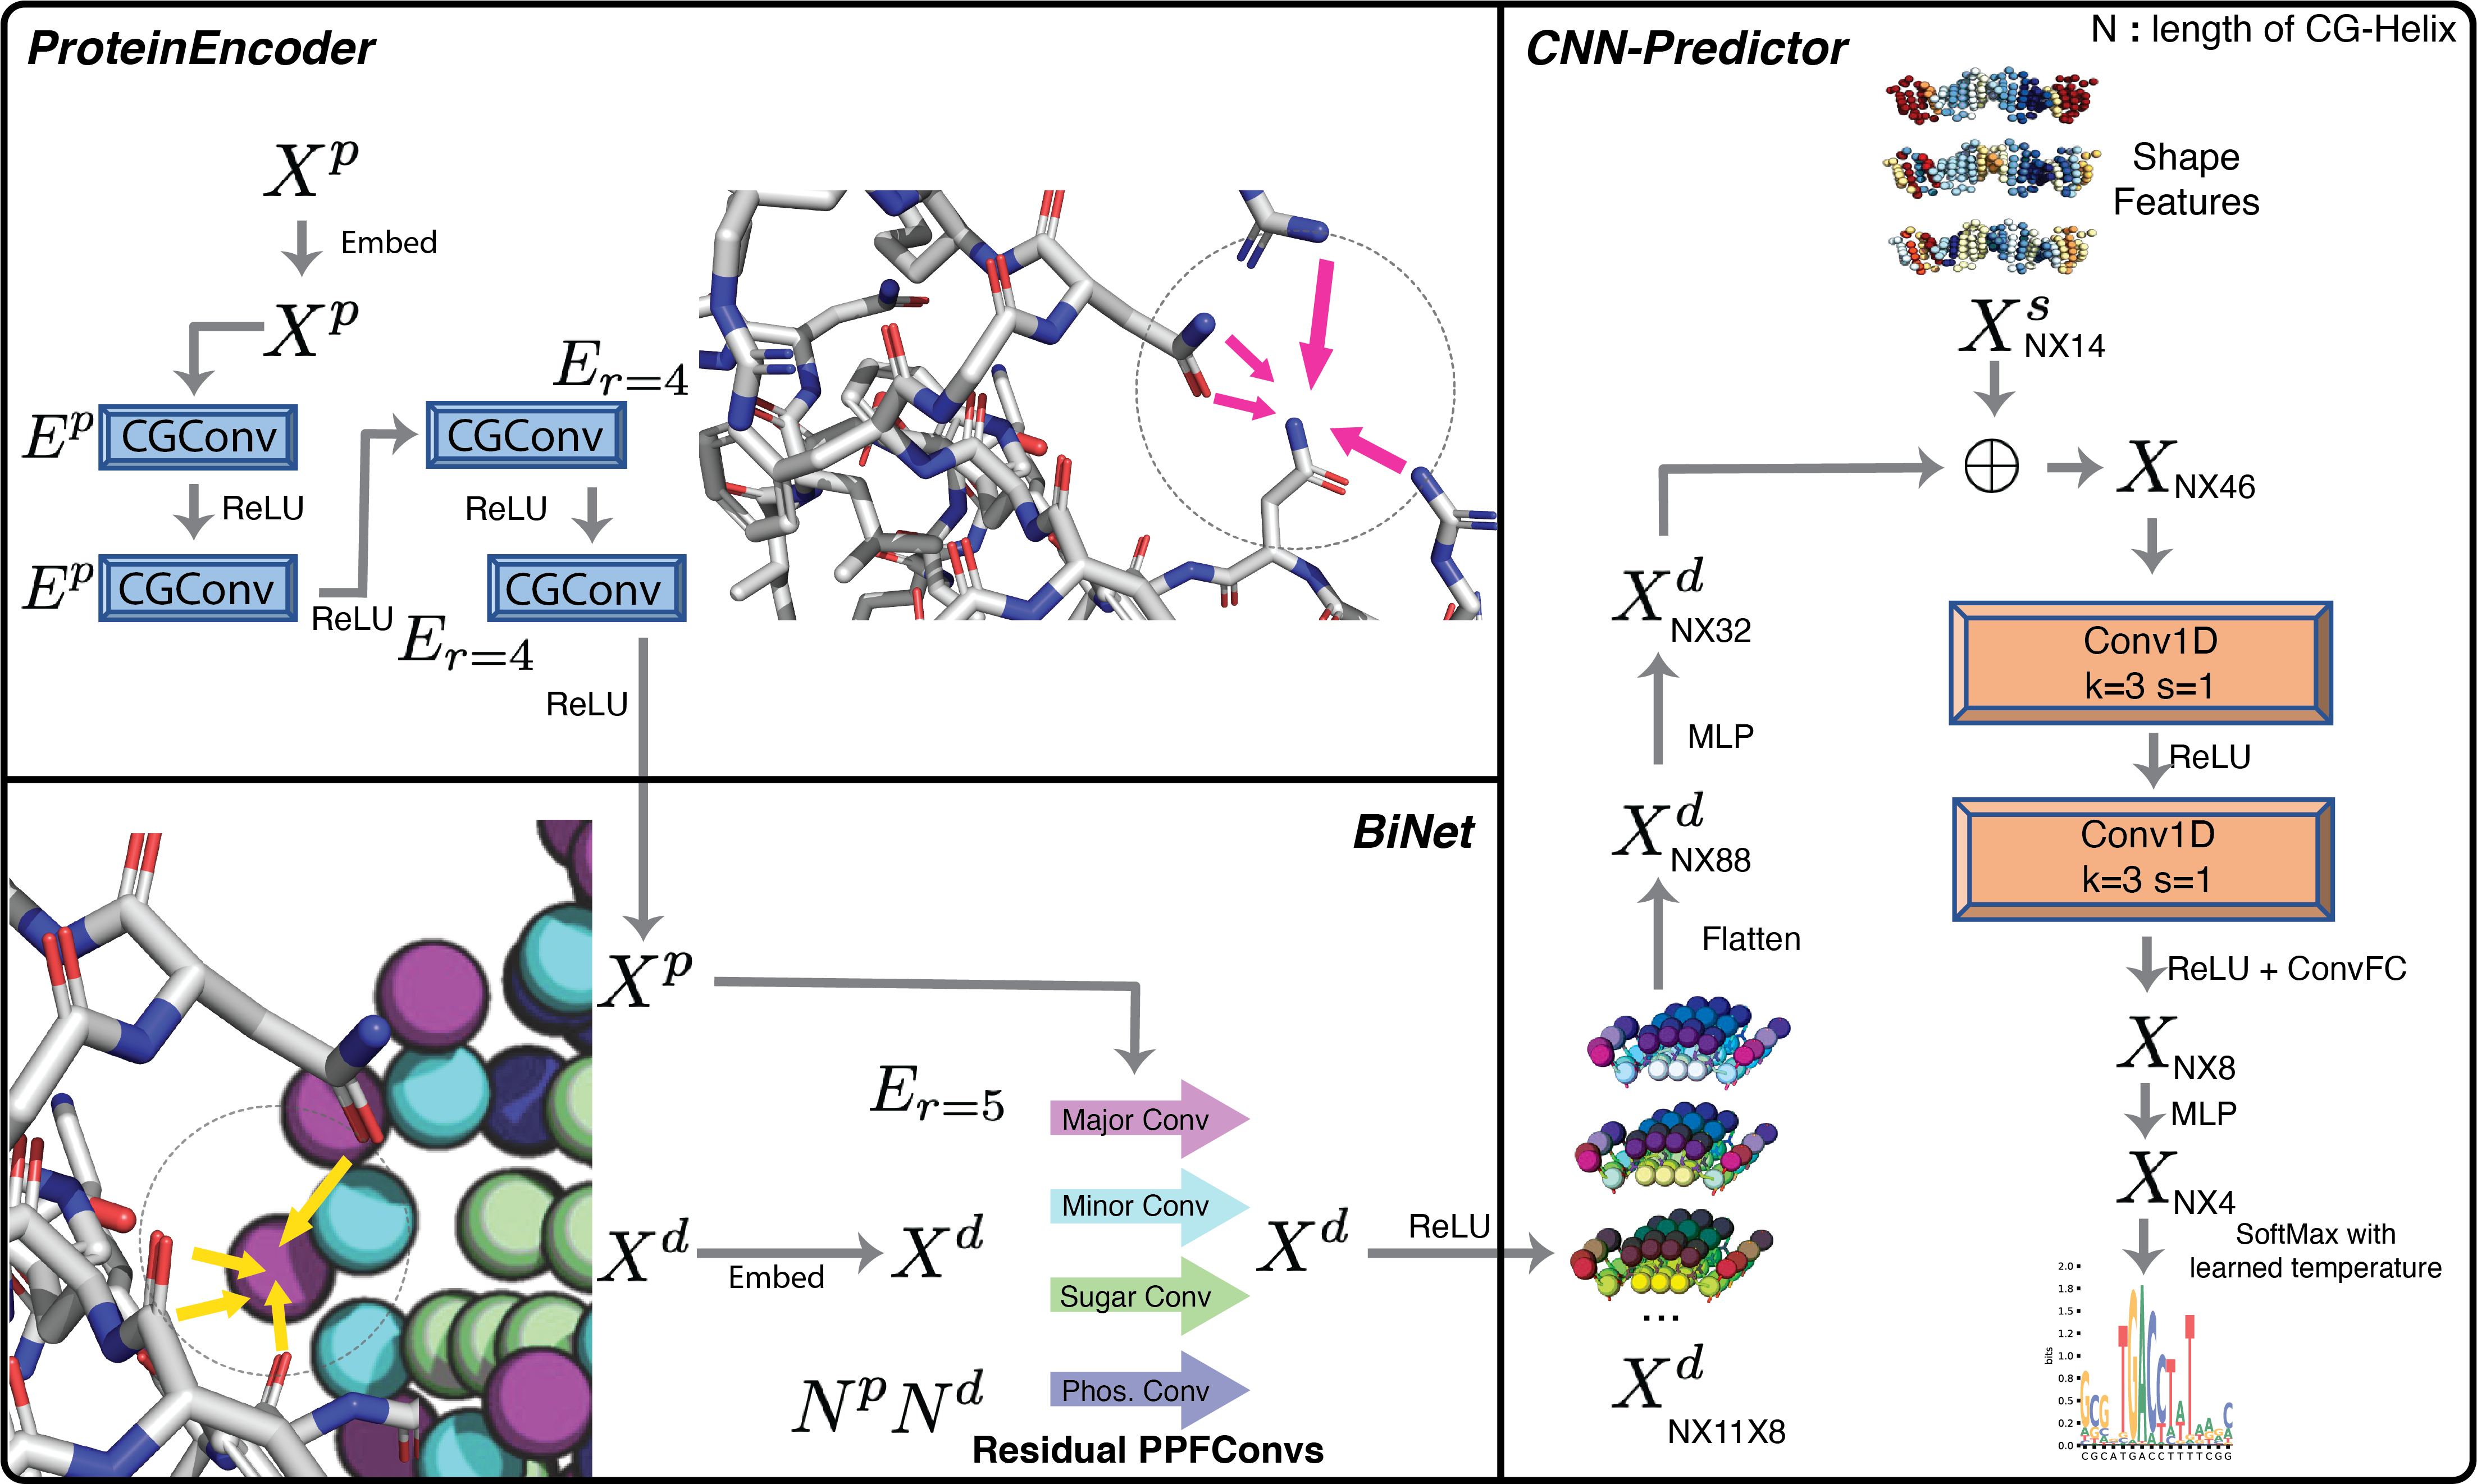
\includegraphics[width=\linewidth]{./pdnafigs/figS3.png}
 % archetecture.png: 1149x508 px, 72dpi, 40.53x17.92 cm, bb=0 0 1149 508
    \caption[DeepPBS architecture.]{\textbf{DeepPBS architecture.} The DeepPBS architecture can be compartmentalized into three modules: ProteinEncoder,
which encodes the protein neighborhood through spatial graph convolutions; BiNet, which consists of a network of
bipartite geometric convolutions from the protein graph ($G^p =
(V^p, X^p, E^p, N^p))$ to sym-helix points (DNA) ($G^d = (v^d, X^d, N^d))$; and CNN-Predictor, which flattens the aggregated sym-helix features into a 1D representation, adds shape features ($X^s$),
and applies 1D convolutional layers followed by fully connected prediction layers. The final logits are converted into probability using a SoftMax activation with a learned temperature parameter. $E_{r=x}$ represents edges determined by vertices/points within a specified radius of length $x$. Each sym-helix point is shown as a sphere (1.5 \AA radius) for visibility.}
  \label{fig:pdnaS3}
\end{figure}
\end{center}

\begin{center}
\begin{figure}[H]
  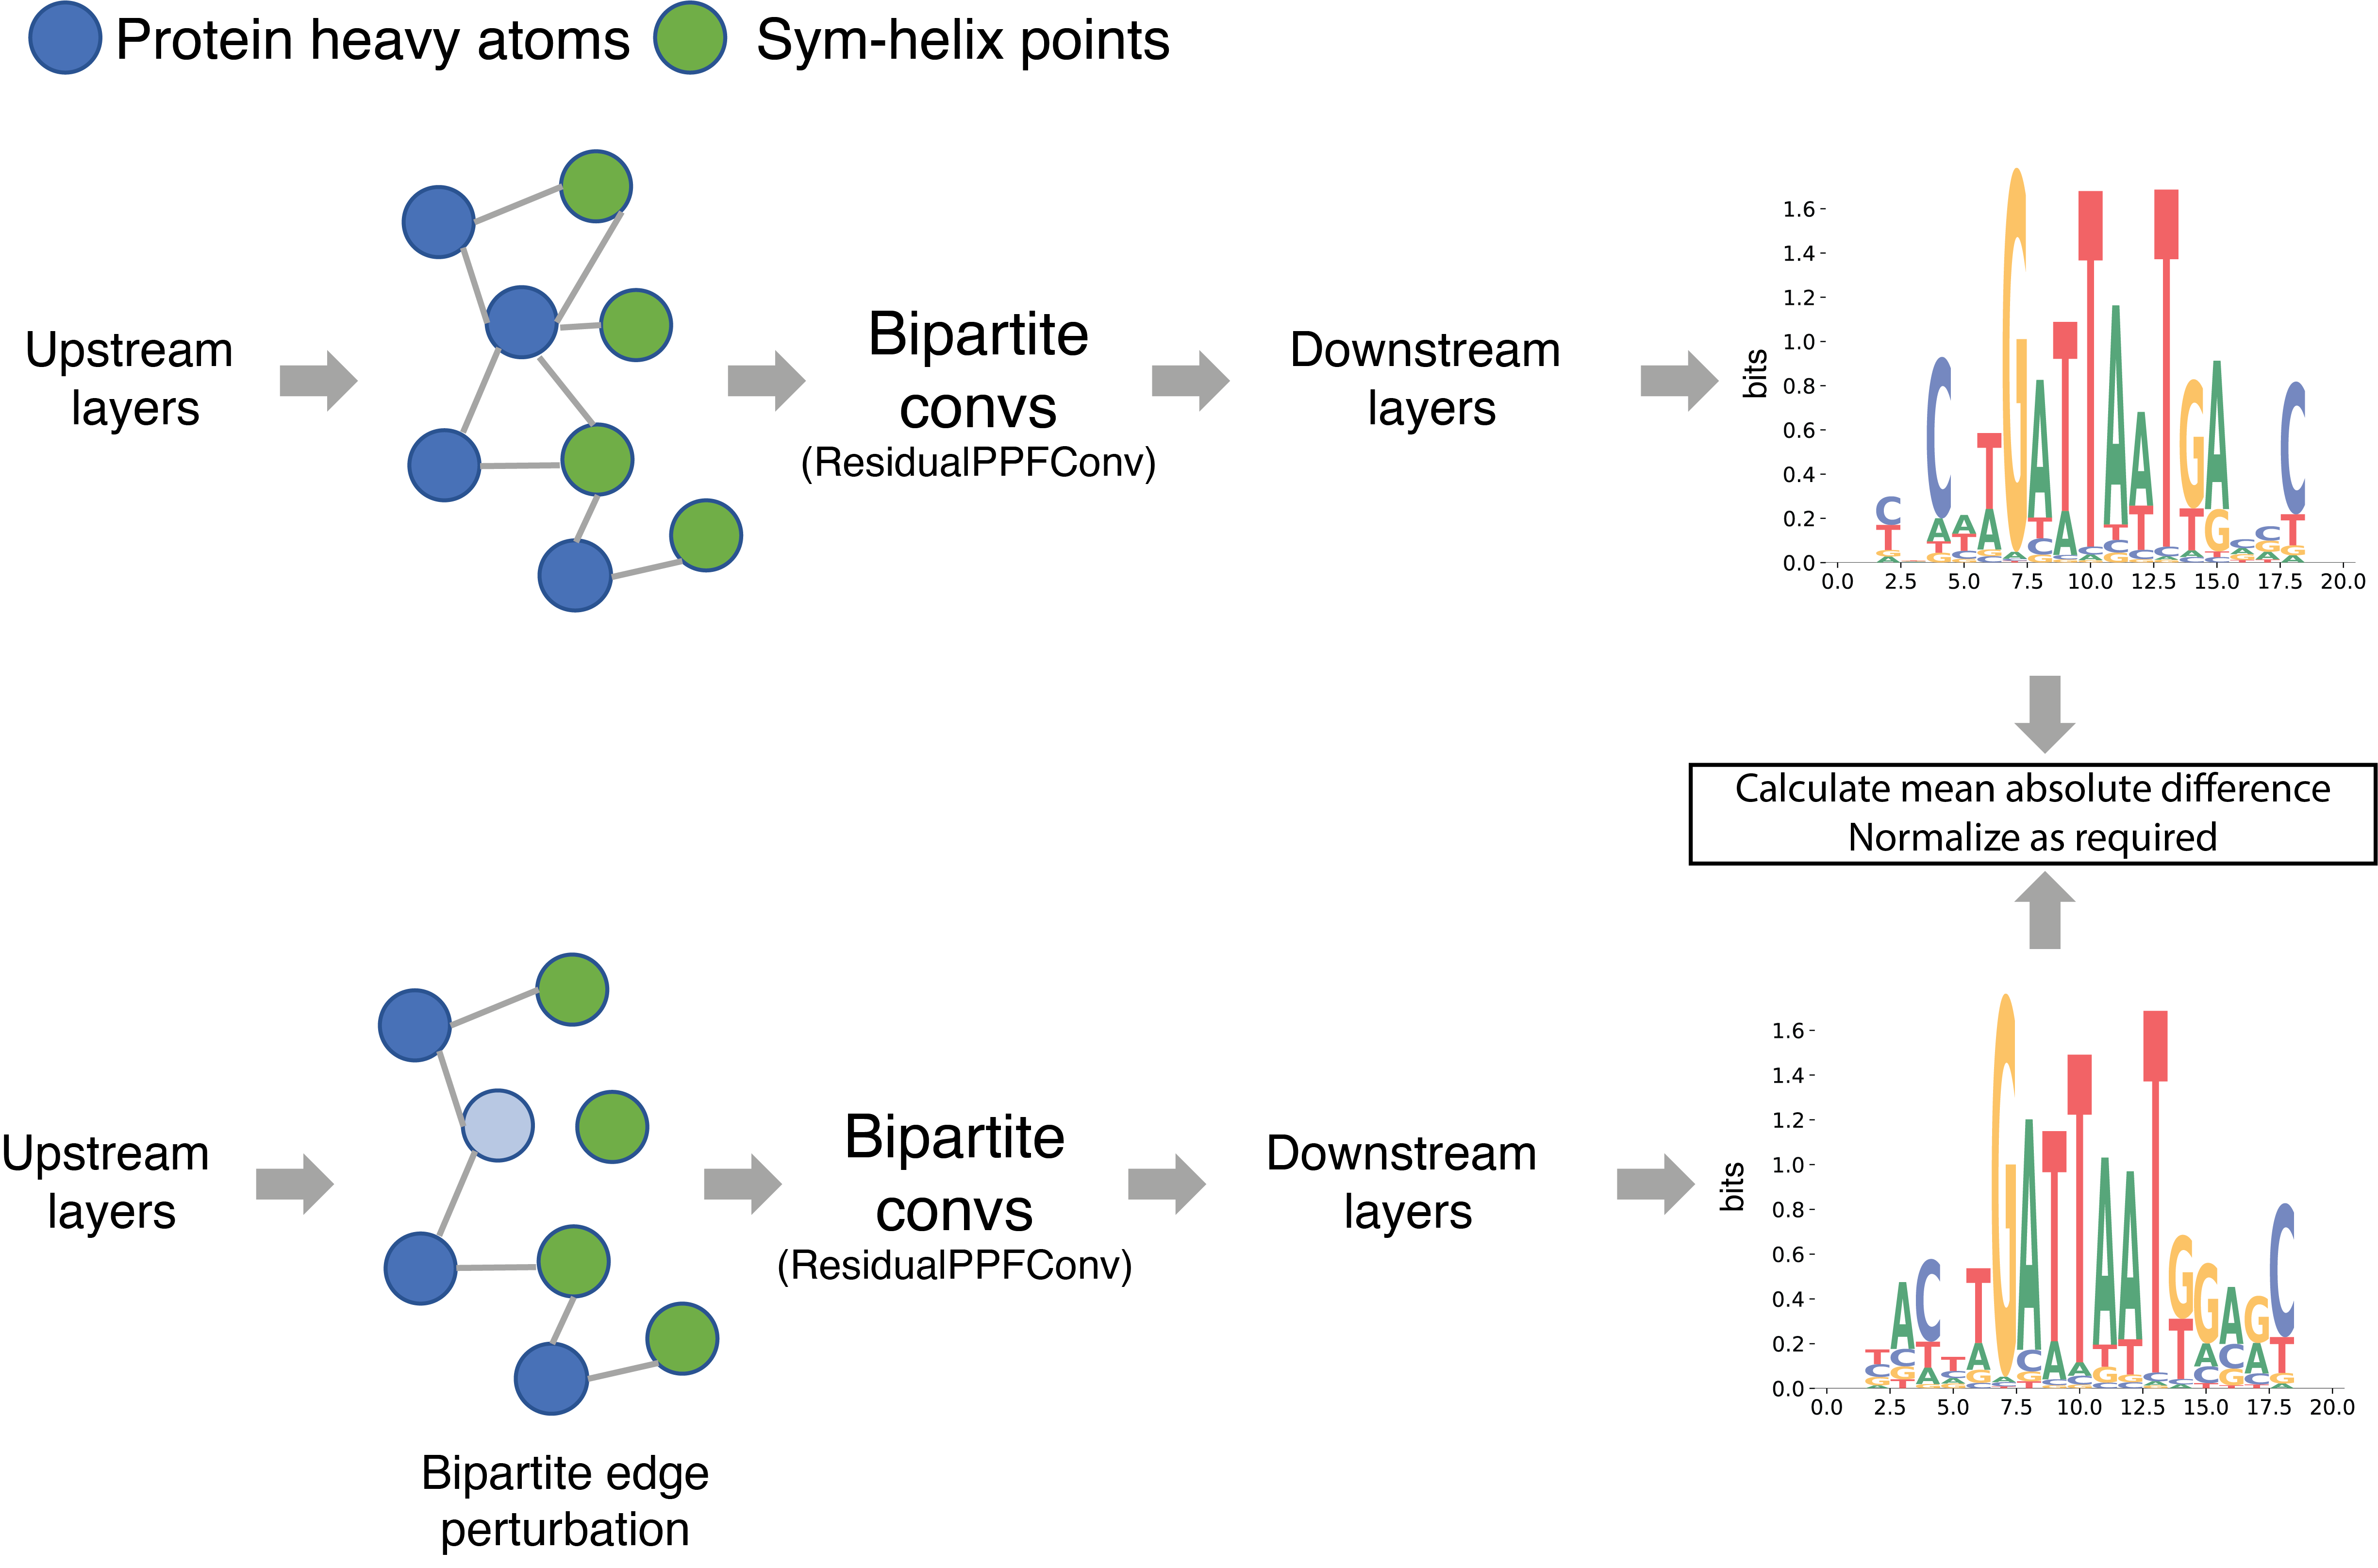
\includegraphics[width=\linewidth]{./pdnafigs/figS4.png}
 % archetecture.png: 1149x508 px, 72dpi, 40.53x17.92 cm, bb=0 0 1149 508
    \caption[Schematic representation of bipartite edge-perturbation process.]{\textbf{Schematic representation of bipartite edge-perturbation process.} Blue circles denote protein heavy atoms.
Green circles represent sym-helix points. In one forward pass, the output is calculated with all edges present. In
another pass, edges corresponding to one protein heavy atom are excluded from the message-passing scheme,
resulting in an alternate output. The difference between the two outputs can be quantified using the mean absolute
difference measure and normalized as needed for interpretation purposes.}
  \label{fig:pdnaS4}
\end{figure}
\end{center}

\begin{center}
\begin{figure}[H]
  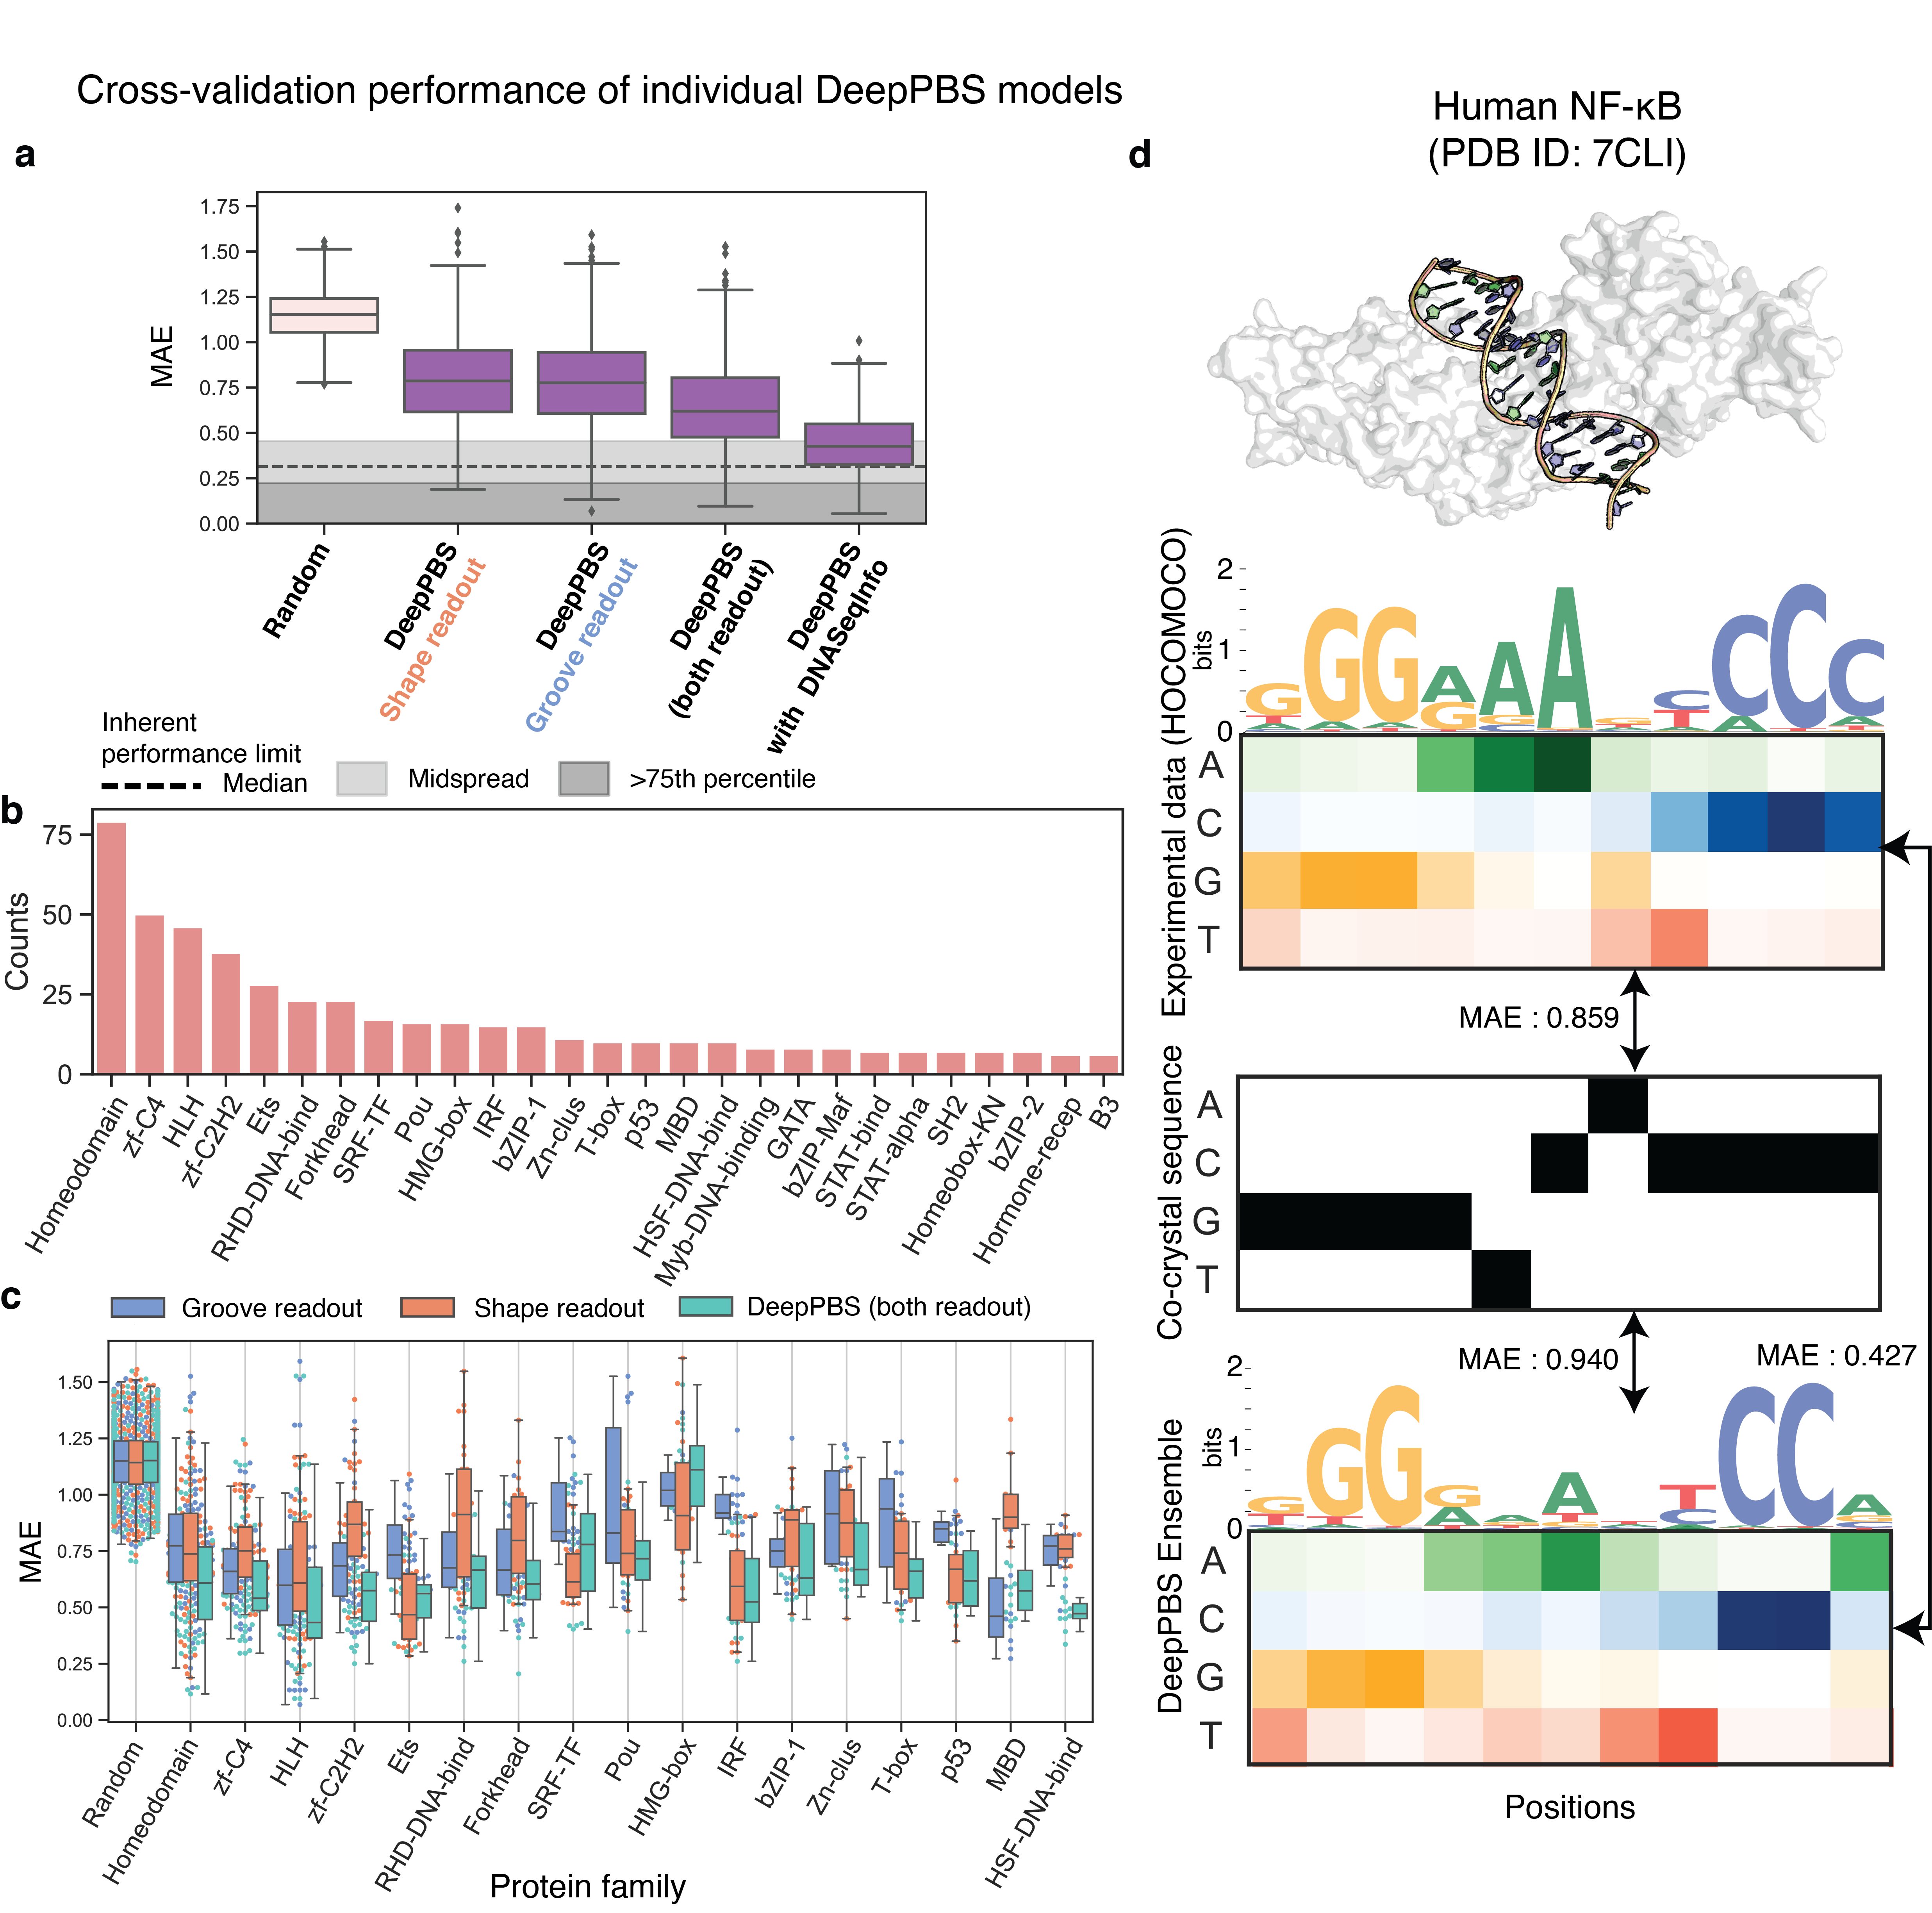
\includegraphics[width=\linewidth]{./pdnafigs/figS5.png}
 % archetecture.png: 1149x508 px, 72dpi, 40.53x17.92 cm, bb=0 0 1149 508
    \caption[Cross-validation performance of DeepPBS for predicting binding specificity across protein families on
experimentally determined structures.]{\textbf{Cross-validation performance of DeepPBS for predicting binding specificity across protein families on experimentally determined structures.} Caption on next page.}
  \label{fig:pdnaS5}
\end{figure}
\addtocounter{figure}{-1}
\begin{figure} [H]
  \caption[Cross-validation performance of DeepPBS for predicting binding specificity across protein families on experimentally determined structures.]{\textbf{Cross-validation performance of DeepPBS for predicting binding specificity across protein families on experimentally determined structures.}({\bf a}) Cross-validation performance of individual trained models for the DeepPBS model and its variations (biological assemblies corresponding to $n$= 523 protein chains (for each box plot)) ({\bf b}) Abundance of various protein families (PFAM annotations) in cross-validation dataset (counts$>$8). ({\bf c}) Cross-validation performance of DeepPBS, along with ‘groove readout’ and ‘shape readout’ variations, across protein families (counts $>$ 8). (Biological assemblies corresponding to $n$ protein chains (for each family), where $n$ is as described in ({\bf b}), total unique $n$= 523) ({\bf d}) Example DeepPBS ensemble prediction on NF-$\kappa$B biological assembly (sampled in benchmark set) containing non-optimal DNA sequence. DeepPBS ensemble prediction on NF-$\kappa$B biological assembly for human (NFKB2, UniProt ID Q00653) is shown in the benchmark dataset. The colored heatmaps (top and bottom) encode probabilities of base identity. The back and white heatmap (center) represents the co-crystal structure. Although the co-crystal structure derived DNA sequence is not of the highest affinity (judging by experimental data from HOCOMOCO), our prediction can circumvent this issue and predict binding specificity levels that are much closer to those observed experimentally. For box plots in ({\bf a}) and ({\bf c}), lower limit represents lower quartile, middle line represents median, and upper limit represents upper quartile. Whiskers do not include outliers.}
\end{figure}
\end{center}

\begin{center}
\begin{figure}[H]
  \includegraphics[width=\linewidth]{./pdnafigs/figS6.png}
 % archetecture.png: 1149x508 px, 72dpi, 40.53x17.92 cm, bb=0 0 1149 508
    \caption[Application of DeepPBS to MD simulation of AlphaFold2- and PDB (2R5Z)-based modeled complex of Exd-
Scr system. ]{\textbf{Application of DeepPBS to MD simulation of AlphaFold2- and PDB (2R5Z)-based modeled complex of Exd-Scr system.} ({\bf a}) Initial structure of simulation. Locations of residues of interest are marked. ({\bf b}) Residue-level RI score over time (averaged per 5 ns window) for residues involved in Exd-DNA flank ineraction. ({\bf c}) Snapshot of interactions by Exd Arg2, Arg3, and Arg5 at 50 ns, 200 ns, and 280 ns, respectively. ({\bf d}) Residue-level RI score over time (averaged 5 ns window) for residues involved in Scr-DNA minor groove interaction. ({\bf e}) Snapshot of interactions by Scr Arg5 and His-12 at 70 ns and 250 ns, respectively. ({\bf f}) Residue-level RI score over time (averaged per 5 ns window) for residues involved in Scr-DNA major groove interaction. ({\bf g}) Snapshot of interactions by Exd Arg58, Lys6, and Ile57 at 70 ns and 250 ns.}
  \label{fig:pdnaS6}
\end{figure}
\end{center}

\begin{center}
\begin{figure}[H]
  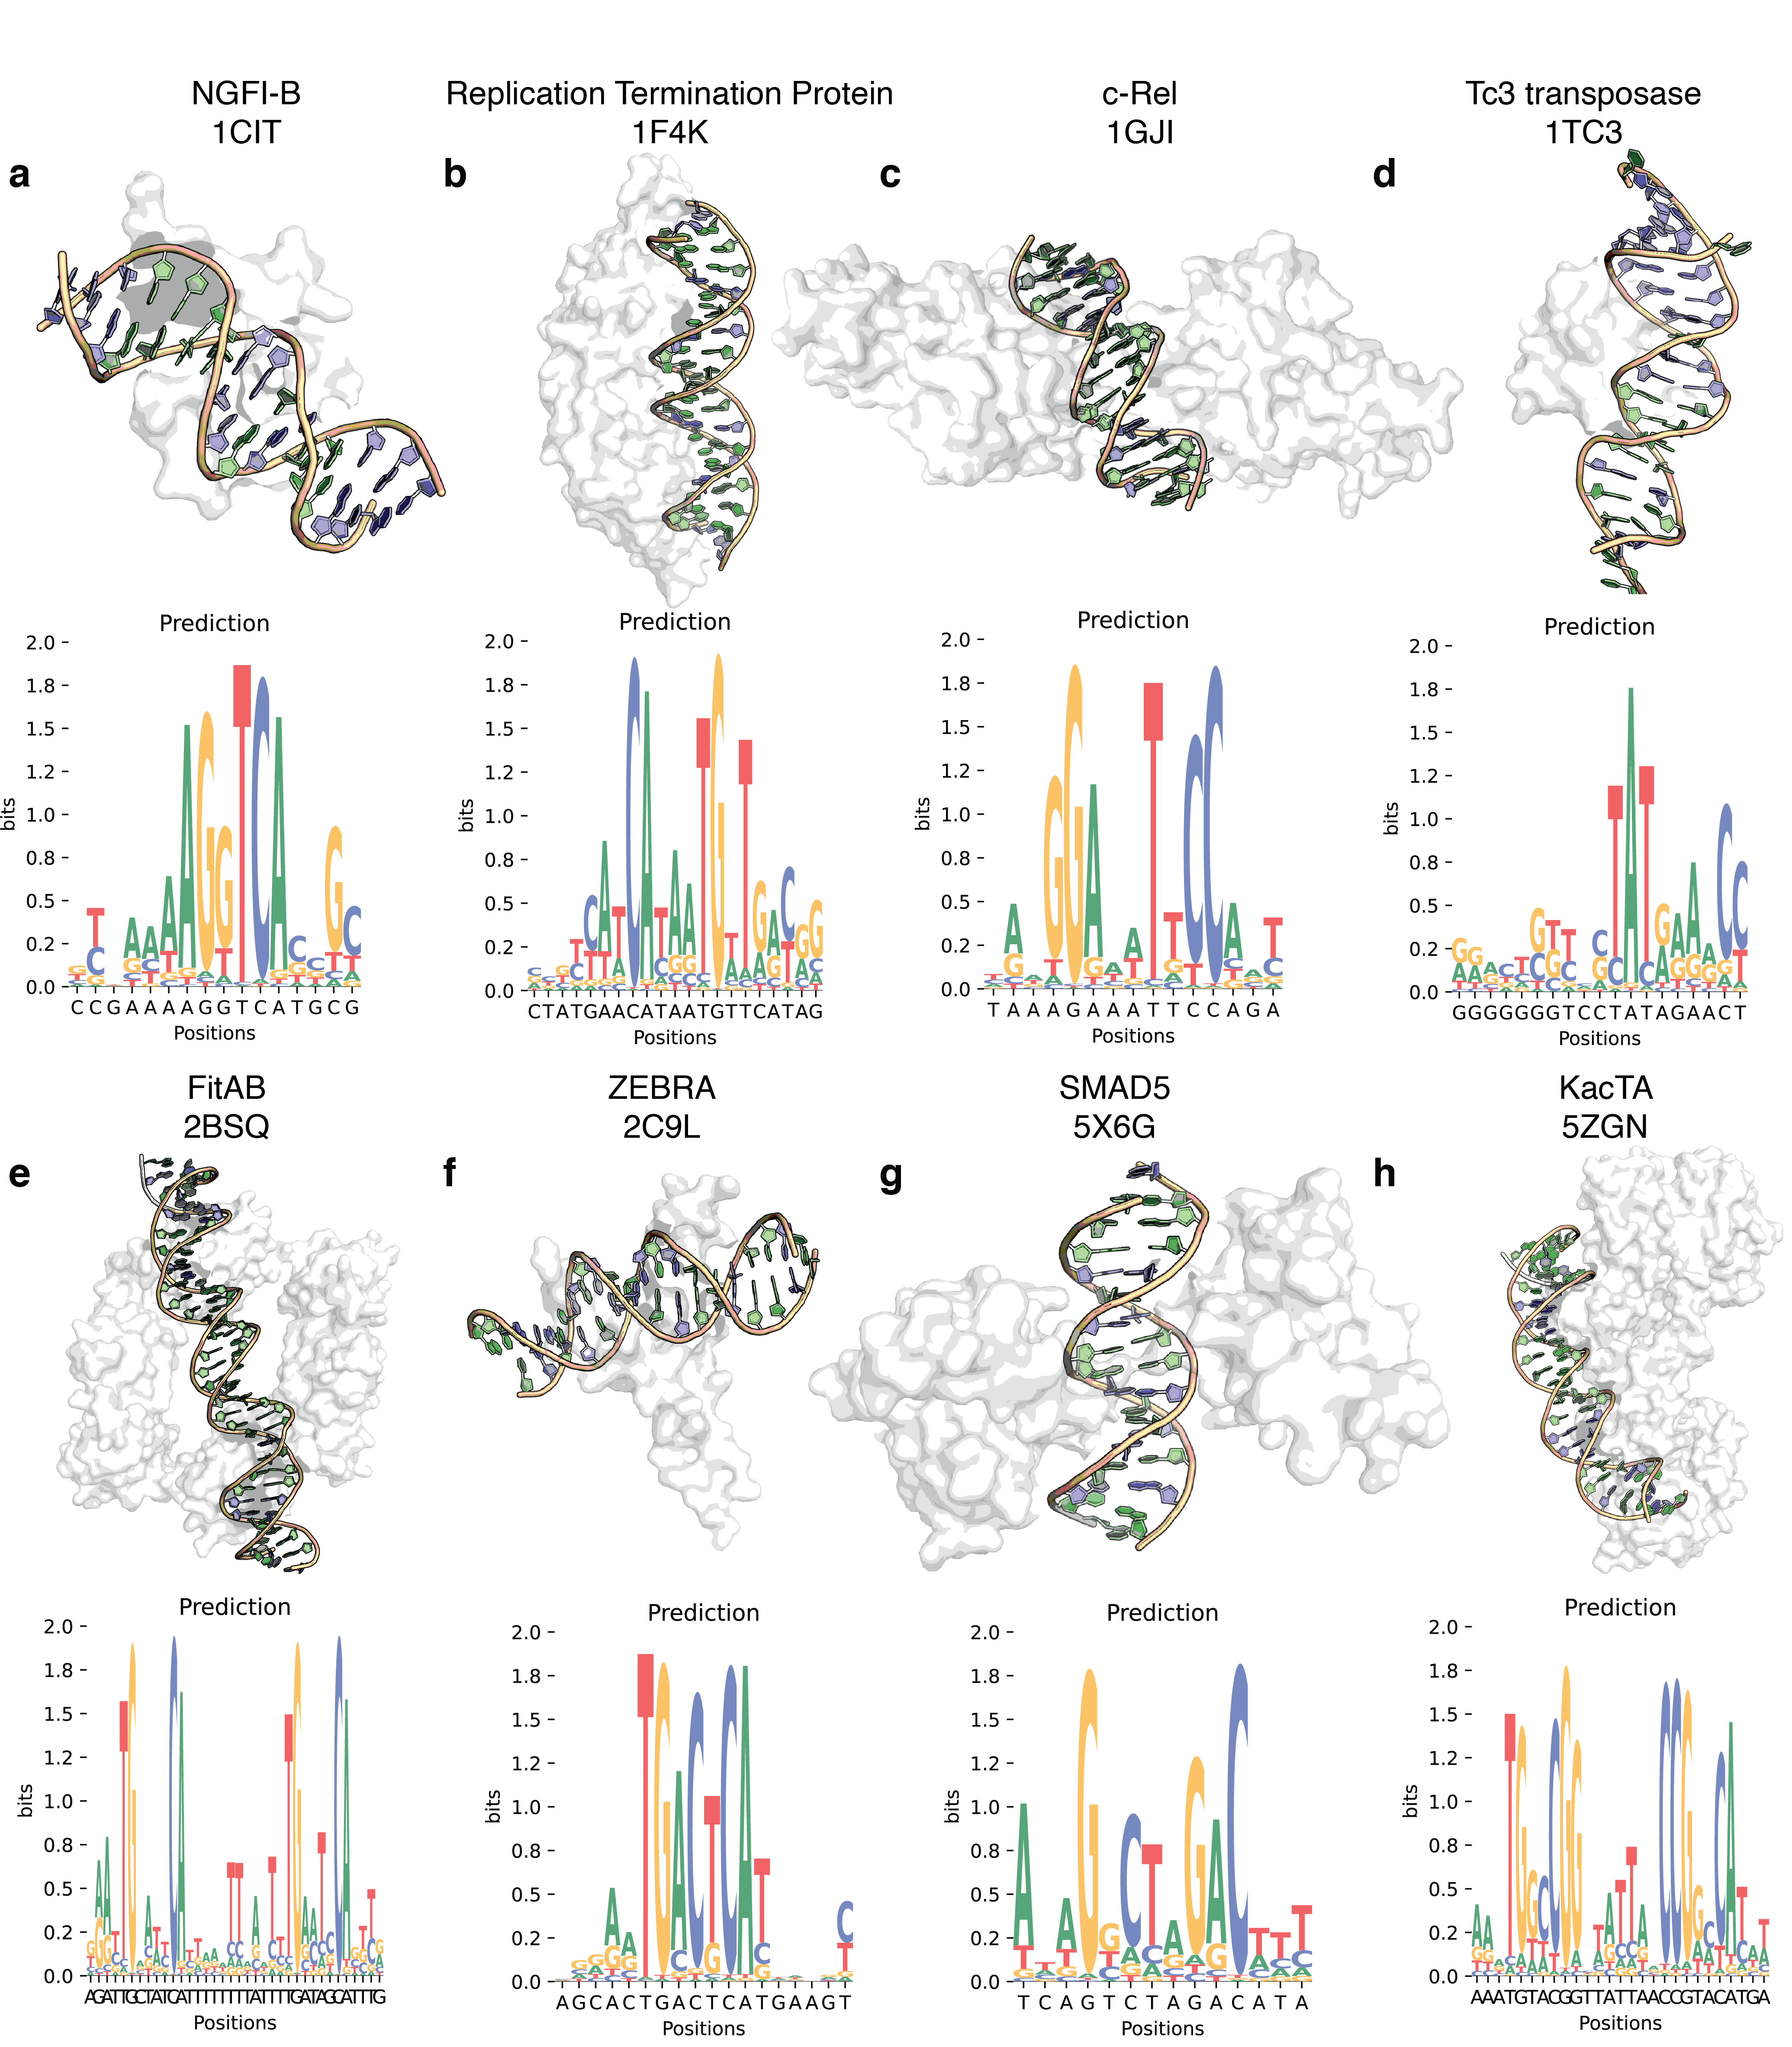
\includegraphics[width=\linewidth]{./pdnafigs/figS7.png}
 % archetecture.png: 1149x508 px, 72dpi, 40.53x17.92 cm, bb=0 0 1149 508
    \caption[Example DeepPBS ensemble predictions on structures of specific DNA binders.]{\textbf{Example DeepPBS ensemble predictions on structures of specific DNA binders.} Specificity data were
unavailable on JASPAR/HOCOMOCO.  ({\bf a}) Monomeric orphan nuclear receptor NGFI-B, ({\bf b}) replication termination protein in bacteria, ({\bf c}) proto-oncogene product c-Rel, ({\bf d}) Tc3 transposase bound to transposon DNA, ({\bf e}) Fitab protein from \textit{Neisseria gonorrhoeae}, ({\bf f}) Epstein-Barr virus ZEBRA protein, ({\bf g}) Smad5-MH1 protein/ palindromic SBE DNA complex, and ({\bf h}) DUF1778 domain-containing kacTA protein.}
  \label{fig:pdnaS7}
\end{figure}
\end{center}

\begin{center}
\begin{figure}[H]
  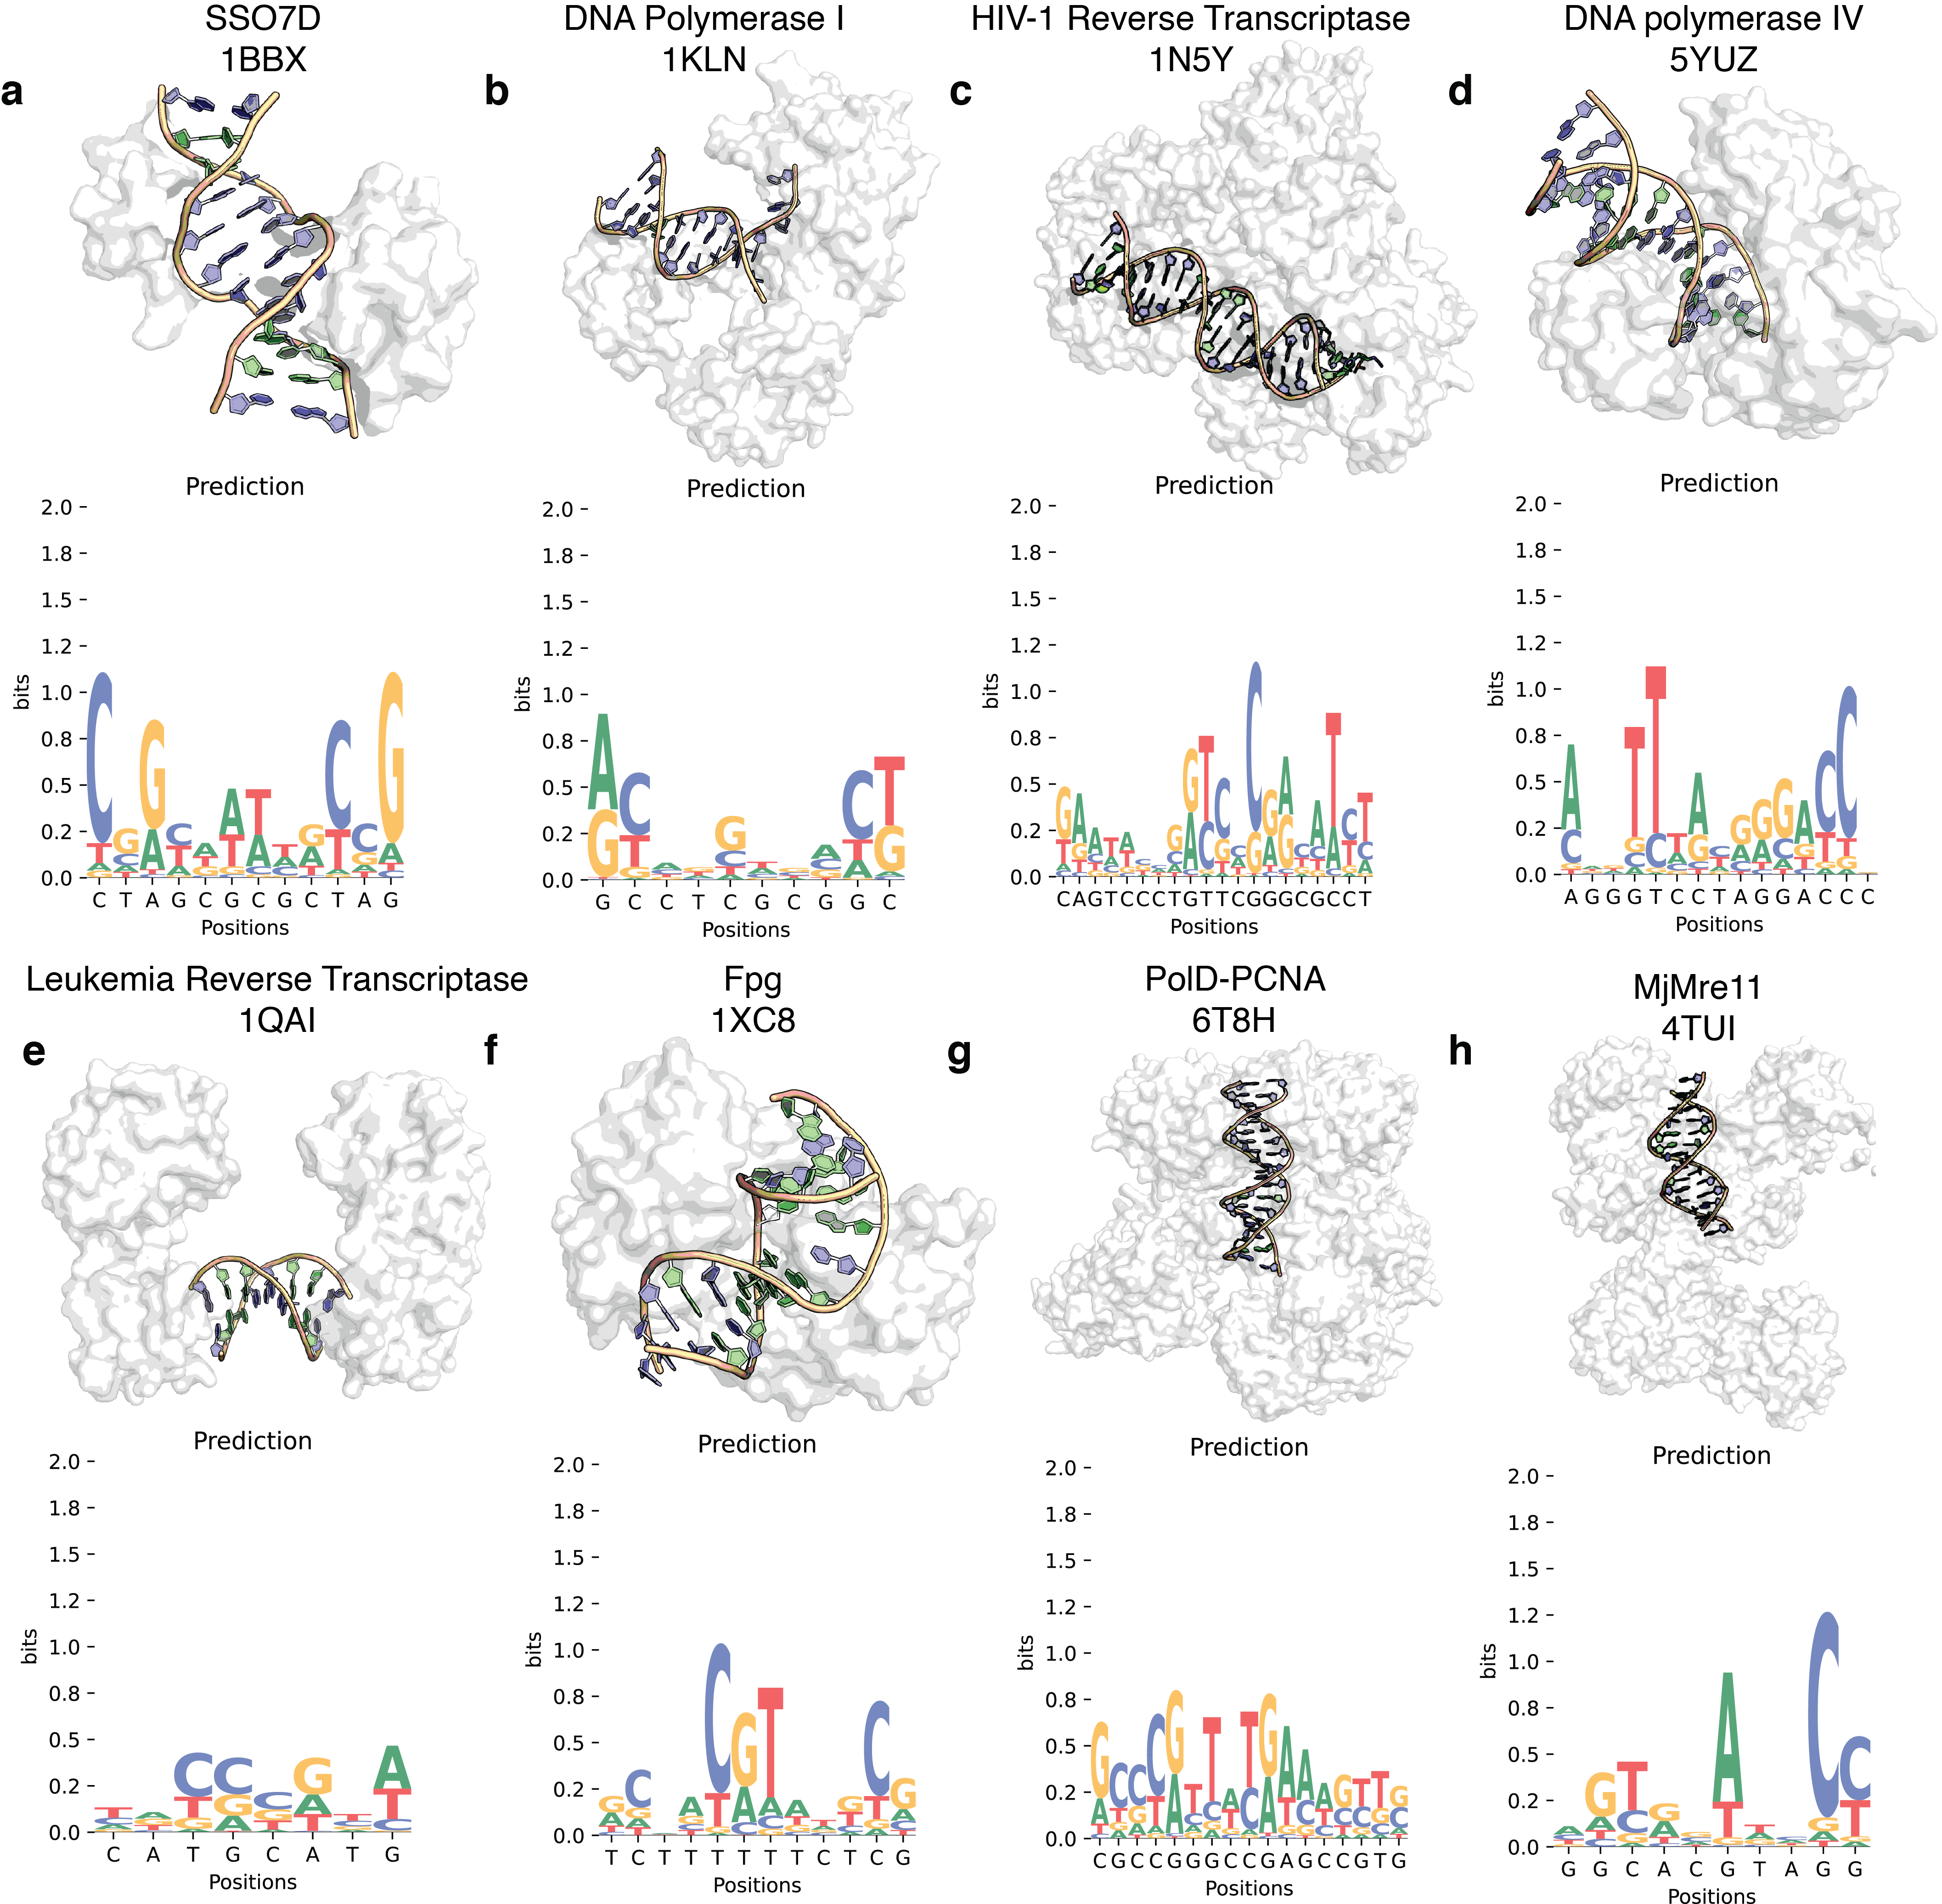
\includegraphics[width=\linewidth]{./pdnafigs/figS8.png}
 % archetecture.png: 1149x508 px, 72dpi, 40.53x17.92 cm, bb=0 0 1149 508
    \caption[Example DeepPBS ensemble predictions on structures of non-specific DNA binders.]{\textbf{Example DeepPBS ensemble predictions on structures of non-specific DNA binders.} ({\bf a}) Sso7D-DNA complex,
({\bf b}) DNA polymerase I Klenow fragment,  ({\bf c}) HIV-1 reverse transcriptase with pre-translocation and post-translocation AZTMP-terminated DNA,  ({\bf d}) DNA polymerase IV,  ({\bf e}) Moloney murine leukemia virus reverse transcriptase,  ({\bf f}) DNA repair enzyme formamidopyrimidine-DNA glycosylase (Fpg),  ({\bf g}) DNA polymerases in complex with proliferative cell nuclear antigen (PCNA), and  ({\bf h}) DNA damage sensing enzyme \textit{Methanococcus jannaschii} Mre11 (MjMre11).}
  \label{fig:pdnaS8}
\end{figure}
\end{center}

\begin{center}
\begin{figure}[H]
  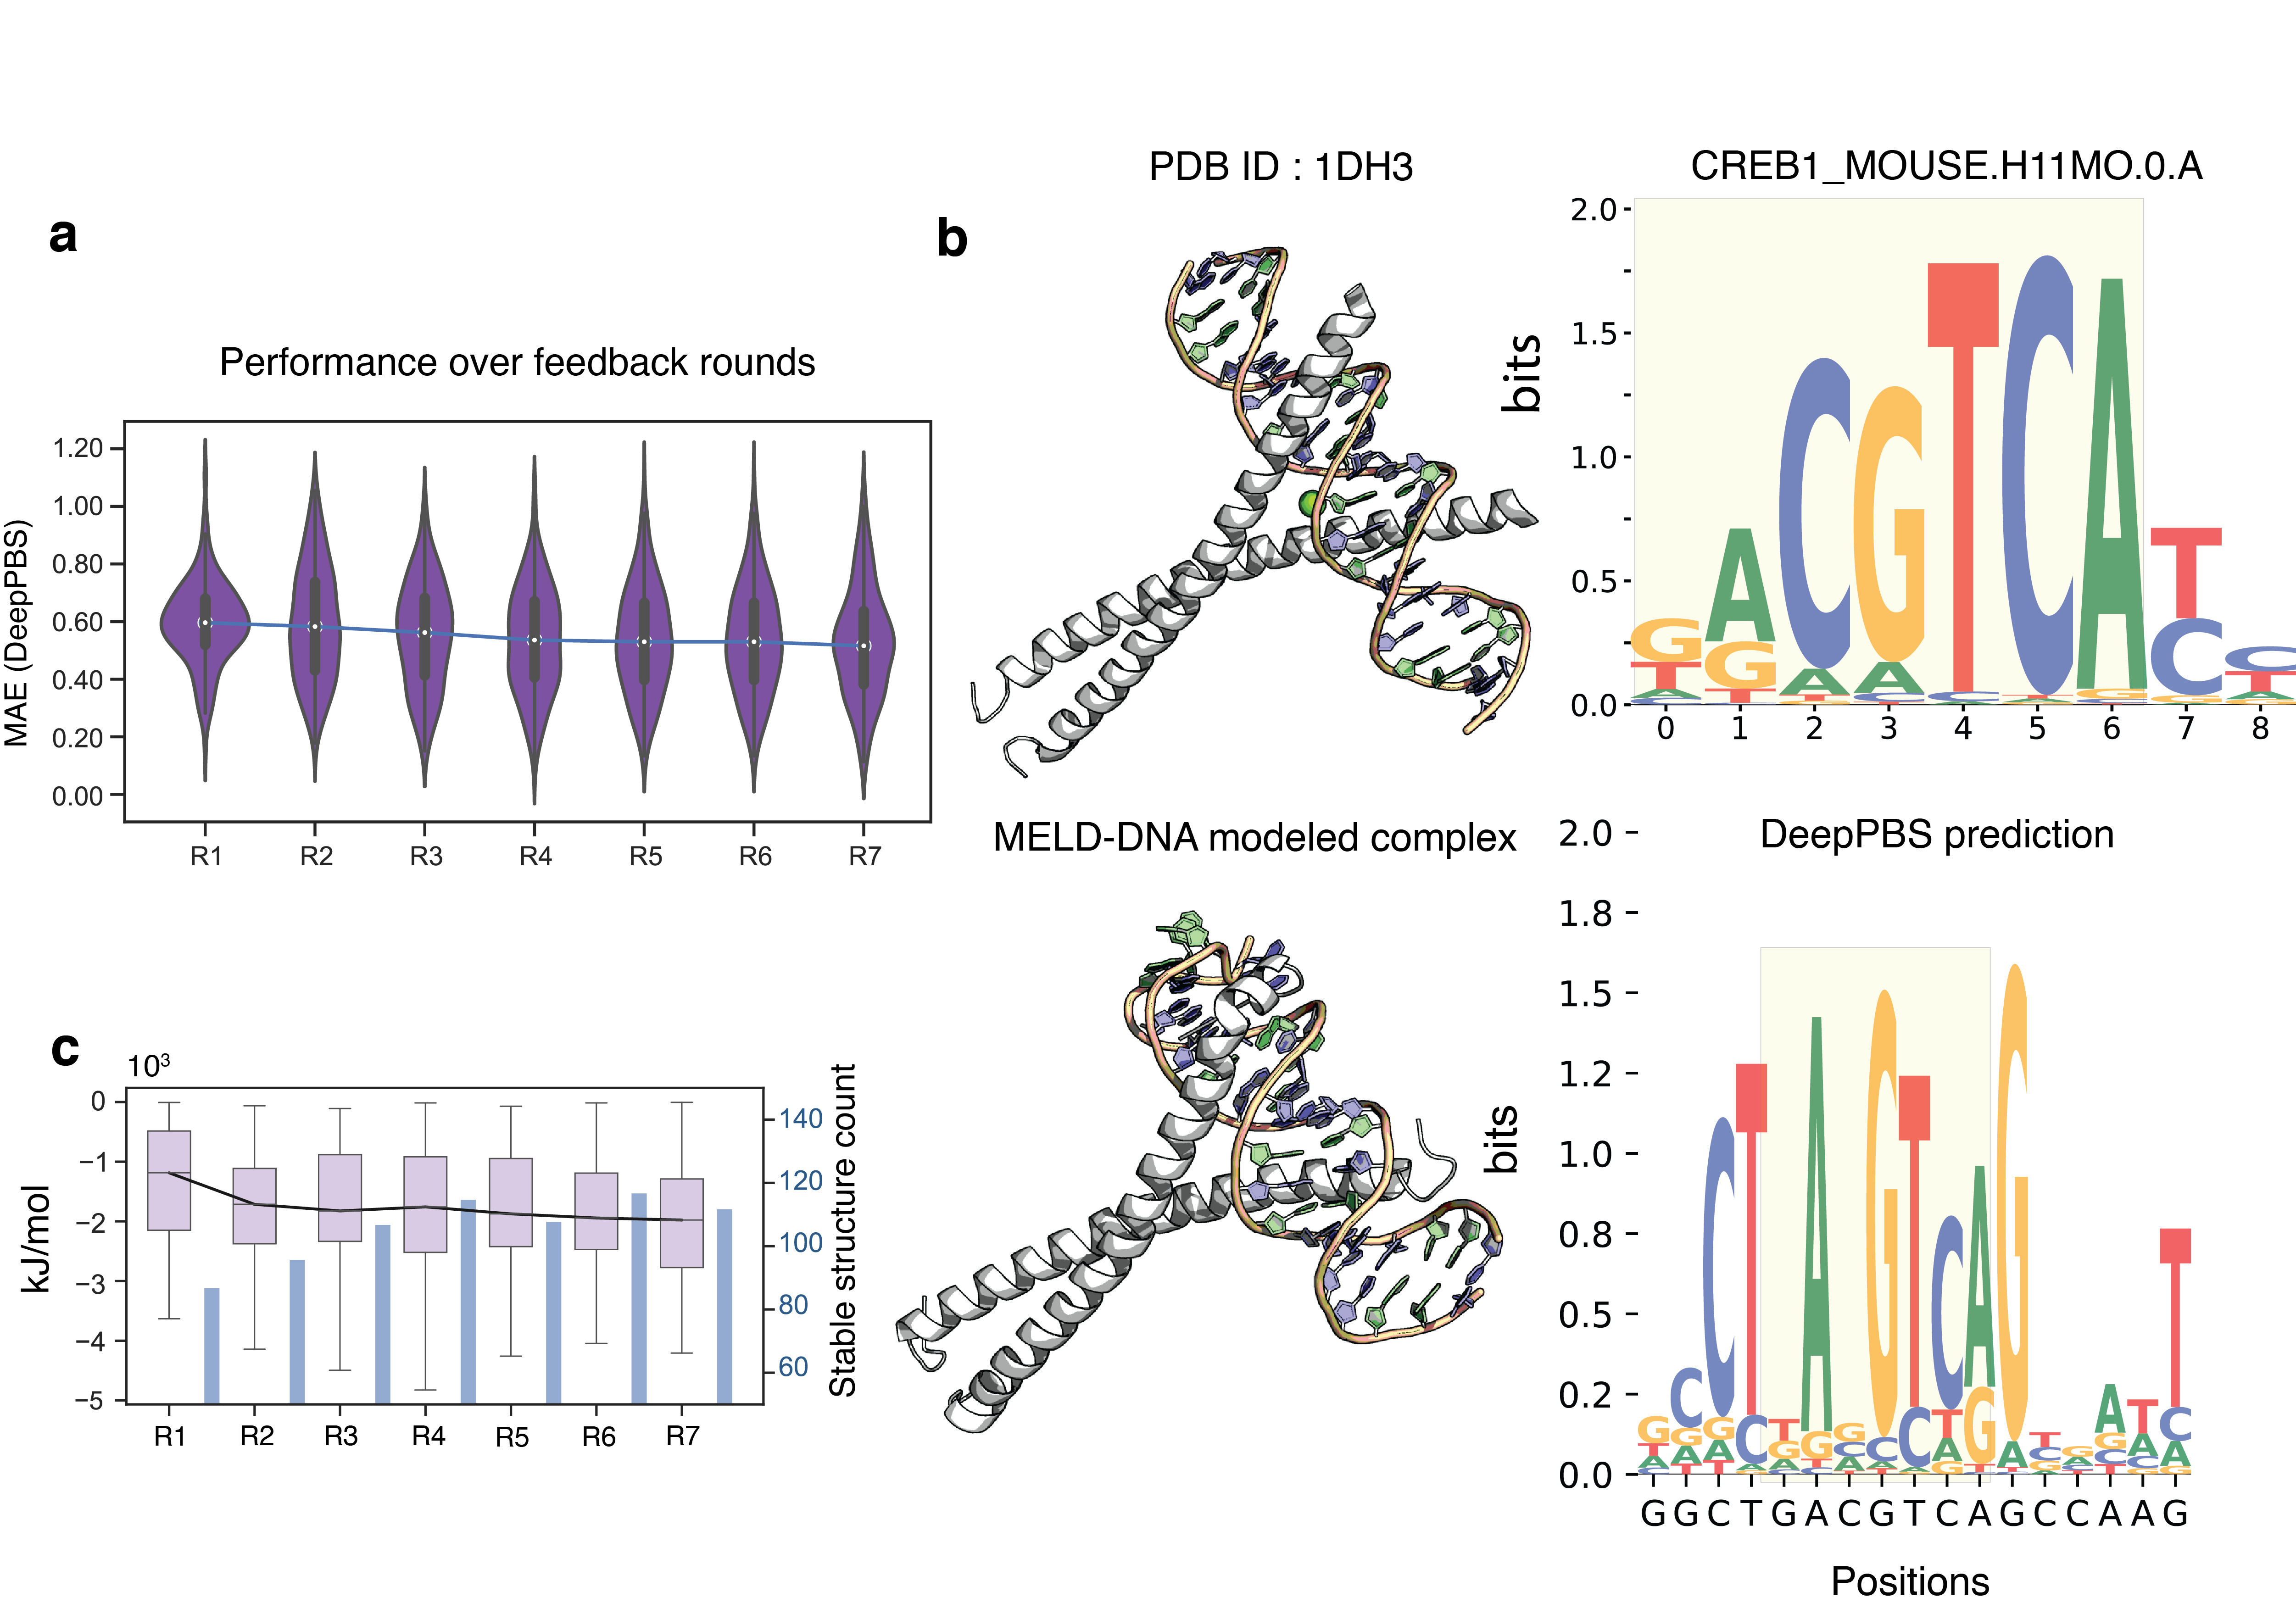
\includegraphics[width=\linewidth]{./pdnafigs/figS9.png}
 % archetecture.png: 1149x508 px, 72dpi, 40.53x17.92 cm, bb=0 0 1149 508
    \caption[Application of DeepPBS on modeled structures.]{\textbf{Application of DeepPBS on modeled structures.} ({\bf a}) Performance of DeepPBS (best 6-mer overlap) improves as
the feedback loop progresses (corresponding to Fig. 3f) in conjunction with improvement in RFNA complex design. ($n$ = 236 predicted assemblies) ({\bf b}) Example application of DeepPBS on mouse CREB1 dimer bound to DNA modeled
by MELD-DNA (as provided by their authors). ({\bf c}) Calculated MM-PBSA (Supplementary Section 7) vacuum energy
distribution for stable RFNA predictions ($<$0 kJ/mol) and corresponding counts over rounds 1–7 (for $n$ predicted
assemblies for each boxplot, where $n$ is same as stable structure count (corresponding bar plot)). For box plots in ({\bf a})
and ({\bf c}), lower limit represents lower quartile, middle point/line represents median, and upper limit represents upper
quartile.}
  \label{fig:pdnaS9}
\end{figure}
\end{center}

\begin{center}
\begin{figure}[H]
  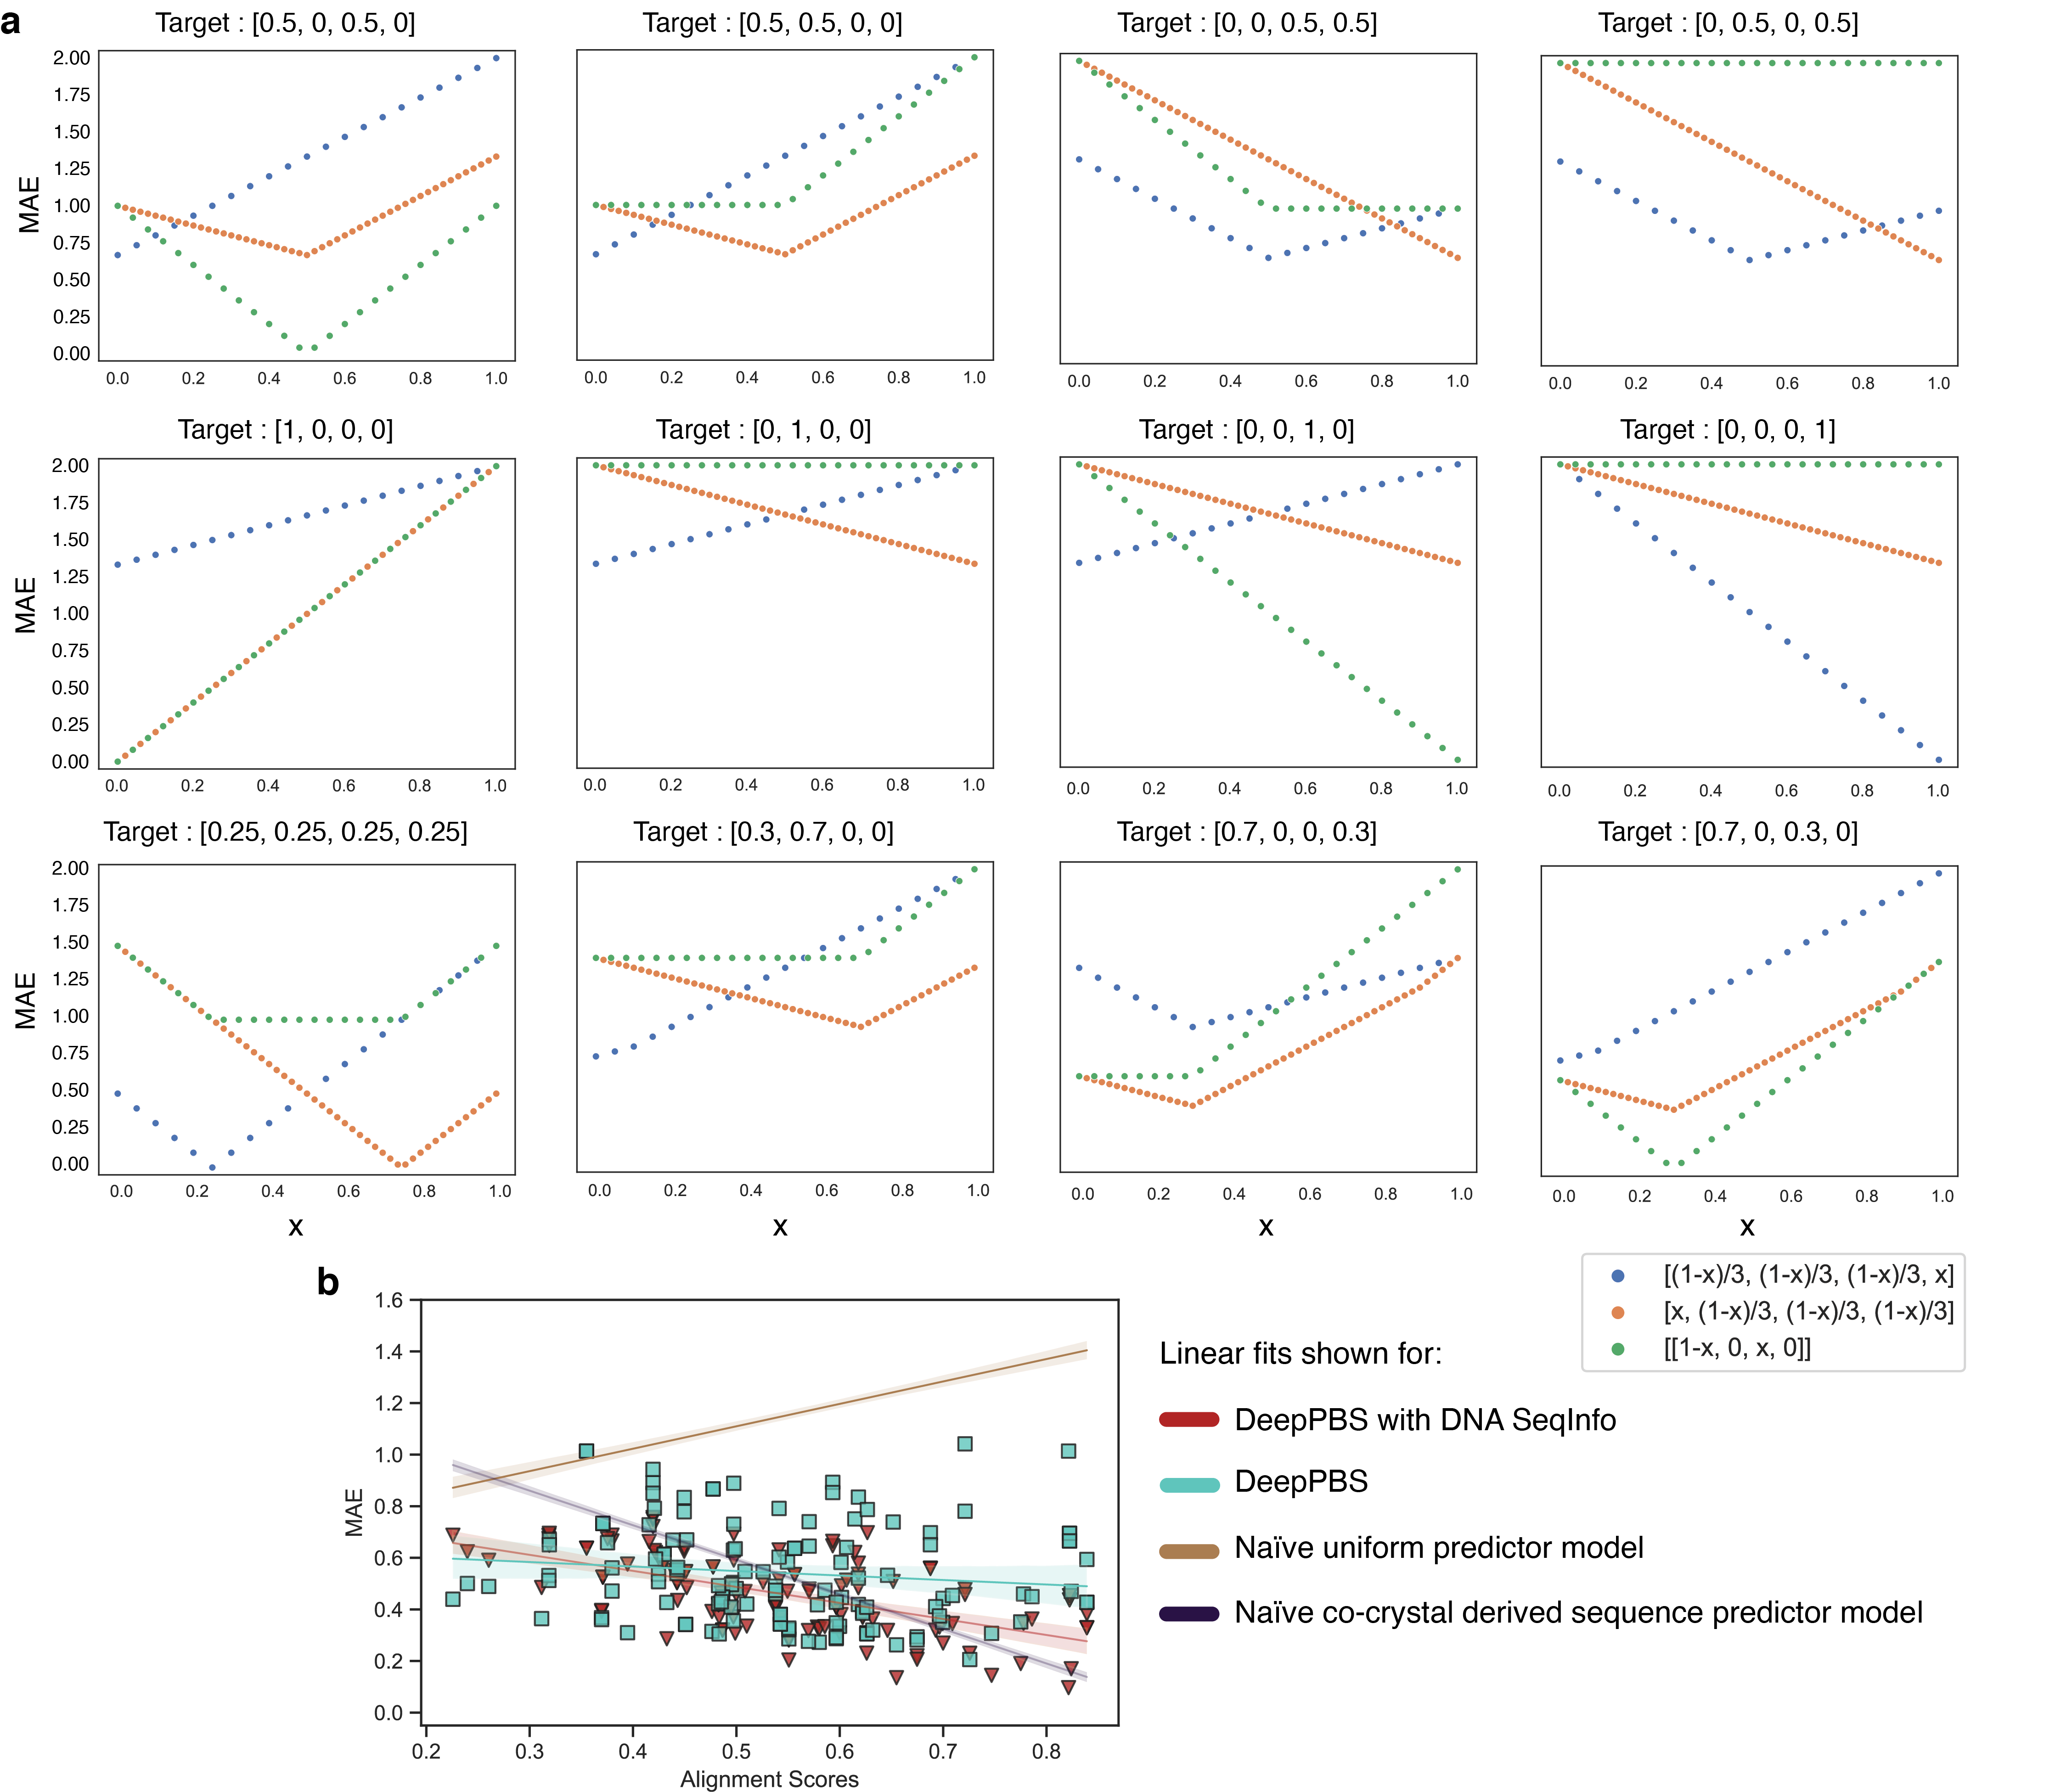
\includegraphics[width=\linewidth]{./pdnafigs/figS10.png}
 % archetecture.png: 1149x508 px, 72dpi, 40.53x17.92 cm, bb=0 0 1149 508
    \caption[Behavior of metric for different target PWM and interpolated predictions.]{\textbf{Behavior of metric for different target PWM and interpolated predictions.} ({\bf a}) Demonstrations of how the MAE
metric behaves for various different target PWM columns and possible predictions (Fig. S10a). The predictions are of three forms, based on interpolated values of a variable $x \in [0,1]$ . Although not an exhaustive set, we hope it helps the reader put into context the behavior of this metric. ({\bf b}) DeepPBS
and DeepPBS with DNA SeqInfo performance on benchmark set in context of two naive models (uniform predictor
and co-crystal structure derived sequence predictor). Lines indicates linear regression fit. Light shaded regions
indicate corresponding 95$\%$ confidence interval computed via bootstrapping mean.}
  \label{fig:pdnaS10}
\end{figure}
\end{center}

\begin{center}
\begin{figure}[H]
  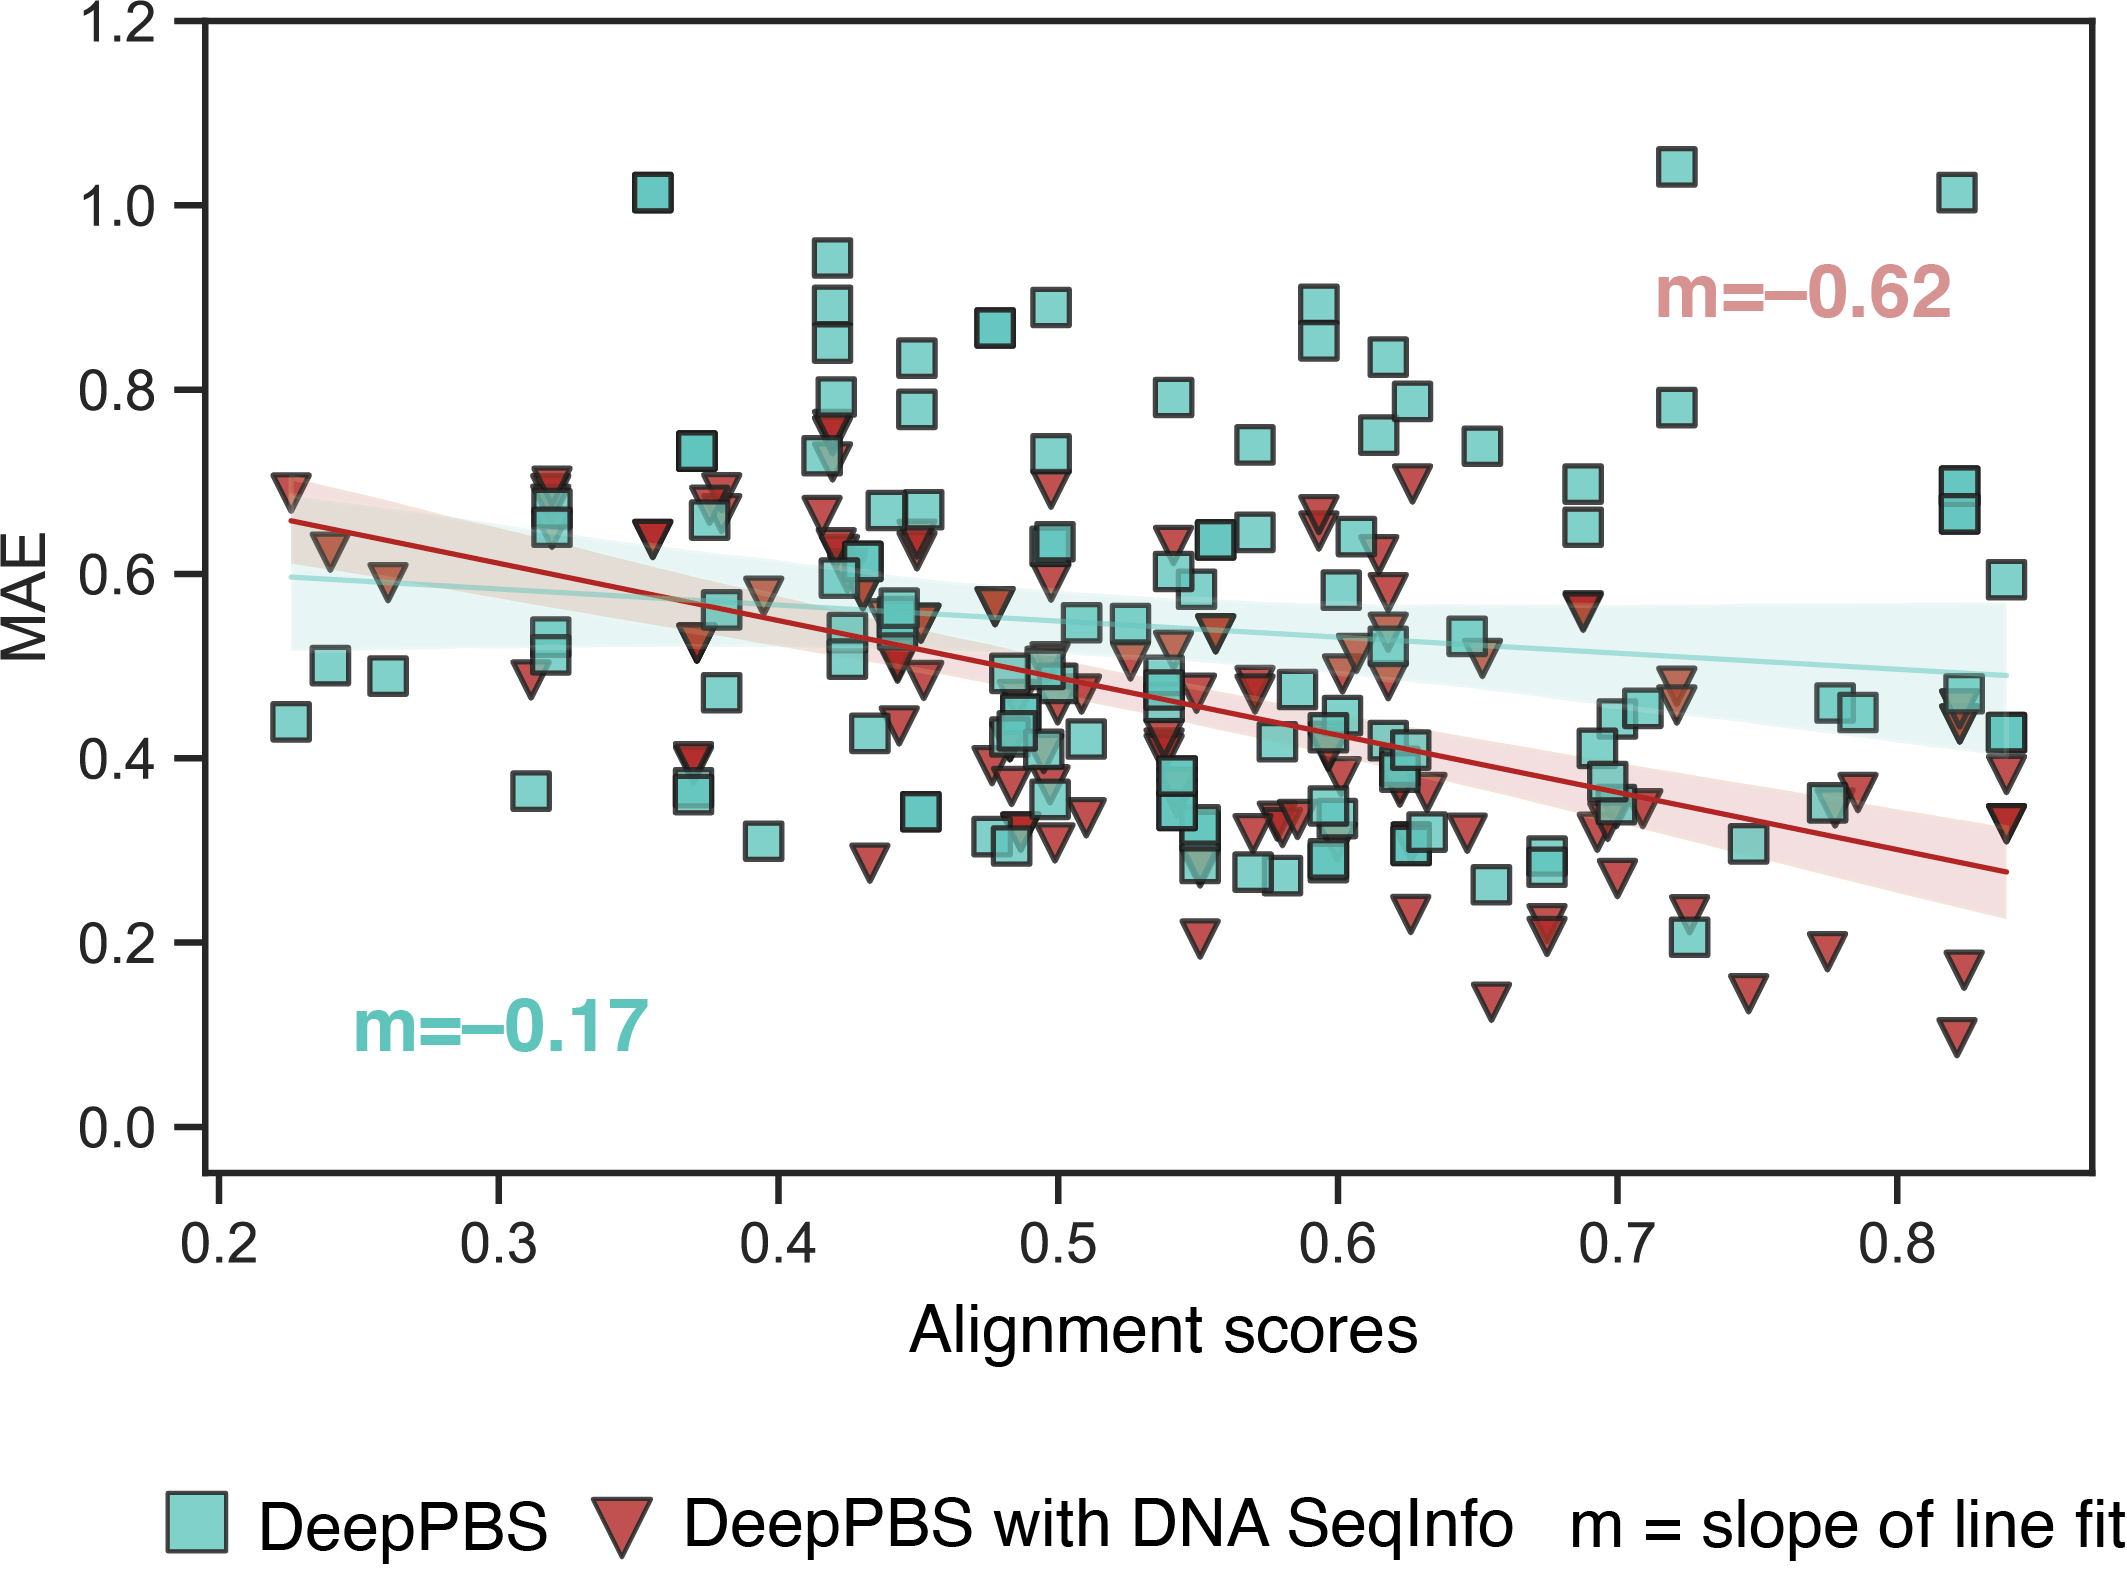
\includegraphics[width=\linewidth]{./pdnafigs/figS11.png}
 % archetecture.png: 1149x508 px, 72dpi, 40.53x17.92 cm, bb=0 0 1149 508
    \caption[MAE equivalent of benchmark performance vs alignment score plot.]{\textbf{MAE equivalent of benchmark performance vs alignment score plot}  showing the bias of the DeepPBS with DNA SeqInfo model compared to the DeepPBS model towards the alignment score of co-crystal DNA structure derived sequence and target PWM. Lines indicates linear regression fit. Light shaded regions indicate corresponding 95$\%$ confidence interval computed via bootstrapping mean.}
  \label{fig:pdnaS11}
\end{figure}
\end{center}

\begin{center}
\begin{figure}[H]
  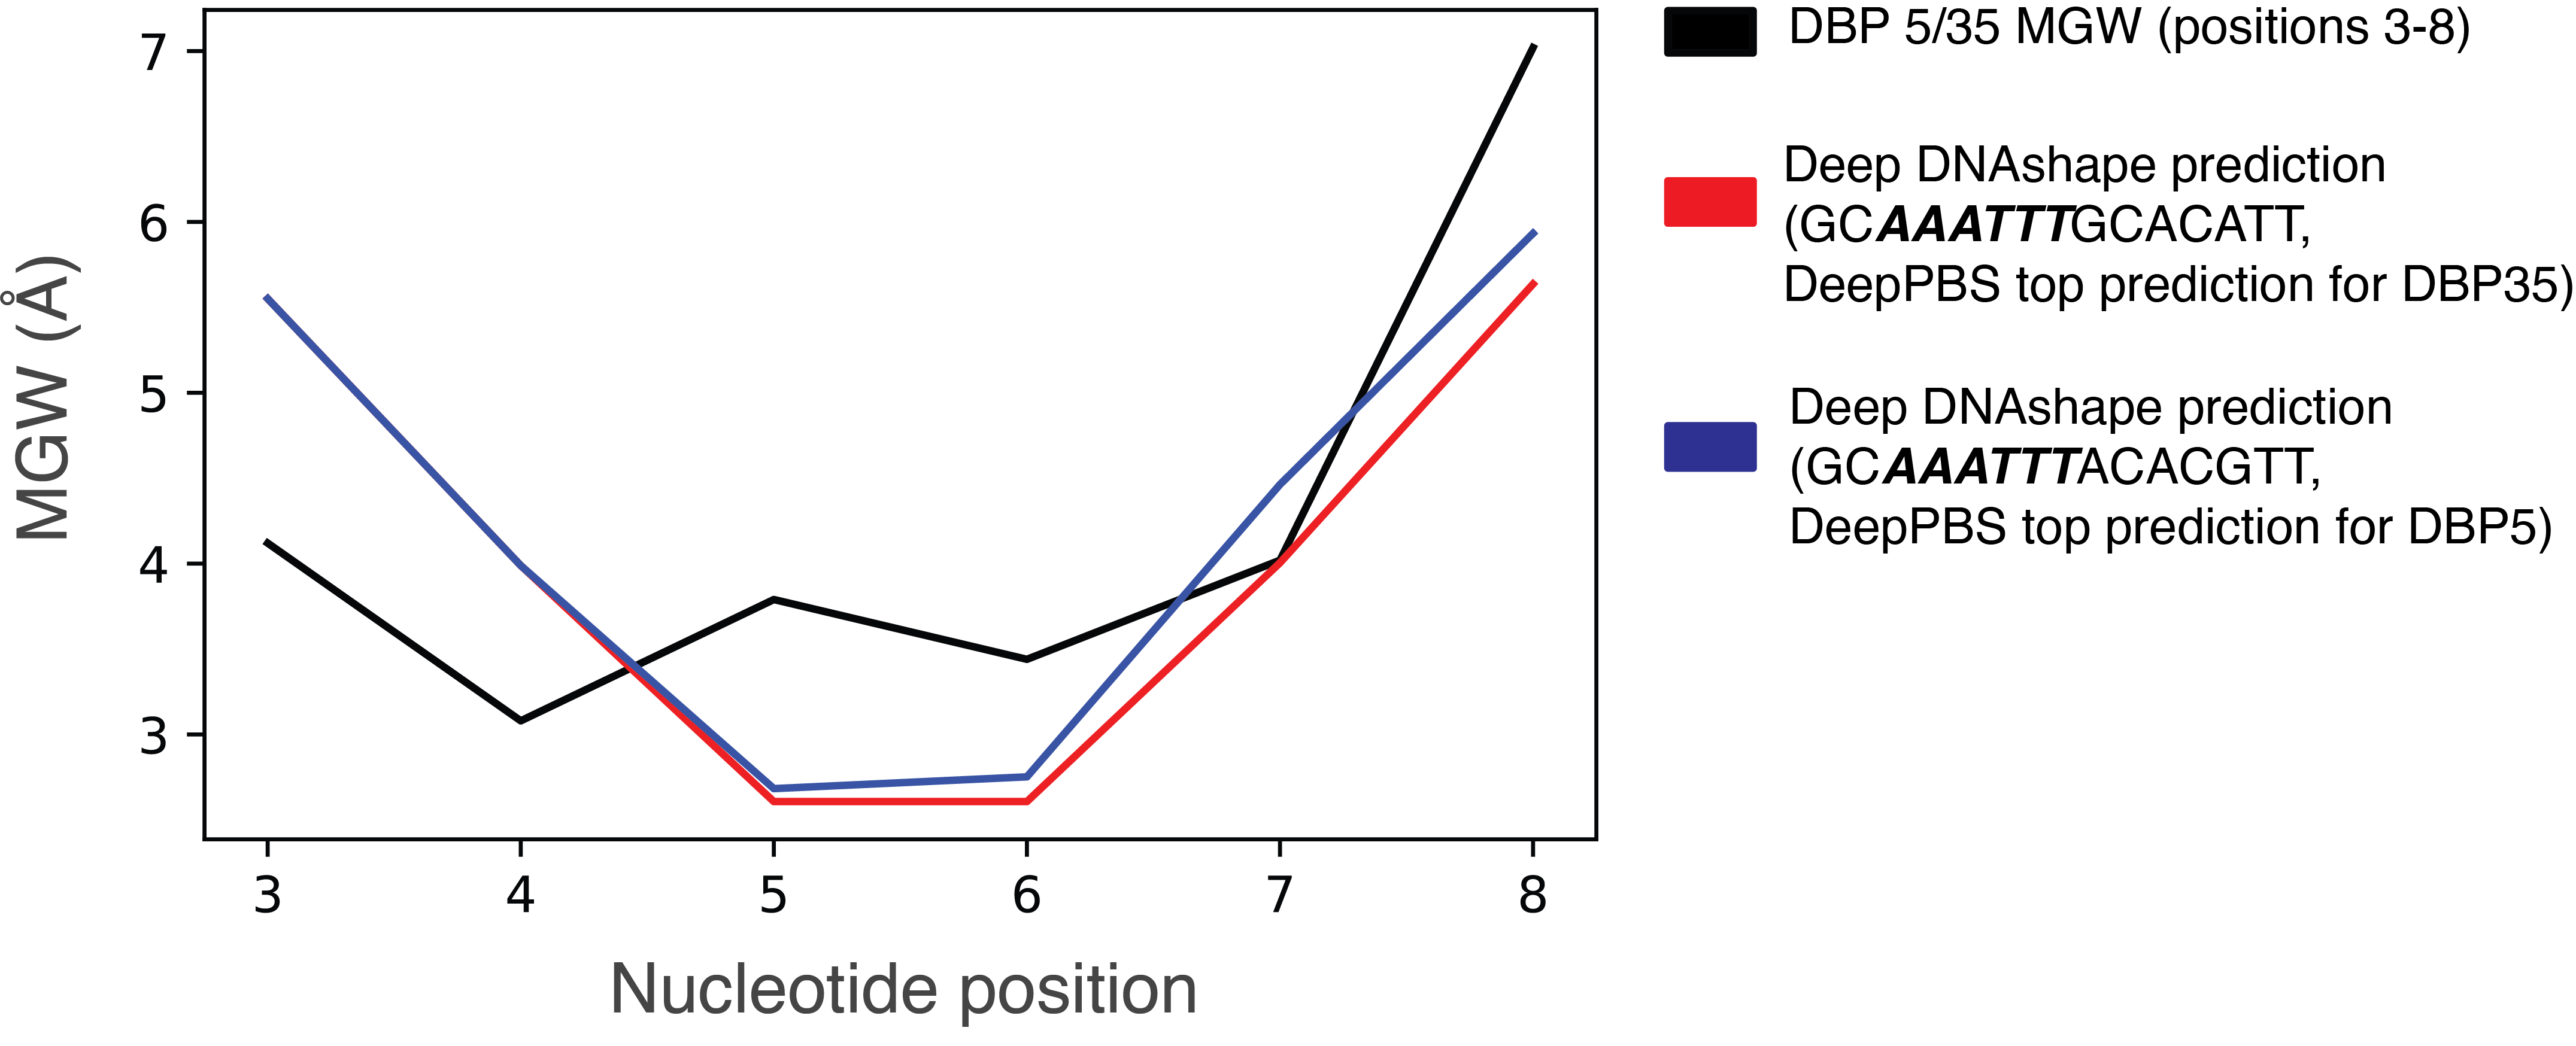
\includegraphics[width=\linewidth]{./pdnafigs/figS12.png}
 % archetecture.png: 1149x508 px, 72dpi, 40.53x17.92 cm, bb=0 0 1149 508
    \caption[Deep DNAshape prediction of the minor groove width (MGW) profile]{\textbf{Deep DNAshape \citep{Li2023} prediction of the minor groove width (MGW) profile} for the sequence AAATTG (top DeepPBS
prediction for the designed model DBP35 and DBP5, positions 3–8) compared to the actual MGW of the DNA in
these designed complexes.}
  \label{fig:pdnaS12}
\end{figure}
\end{center}
%% RNASCAPE SUPP FIGURES
\begin{center}
\begin{figure}[H]
  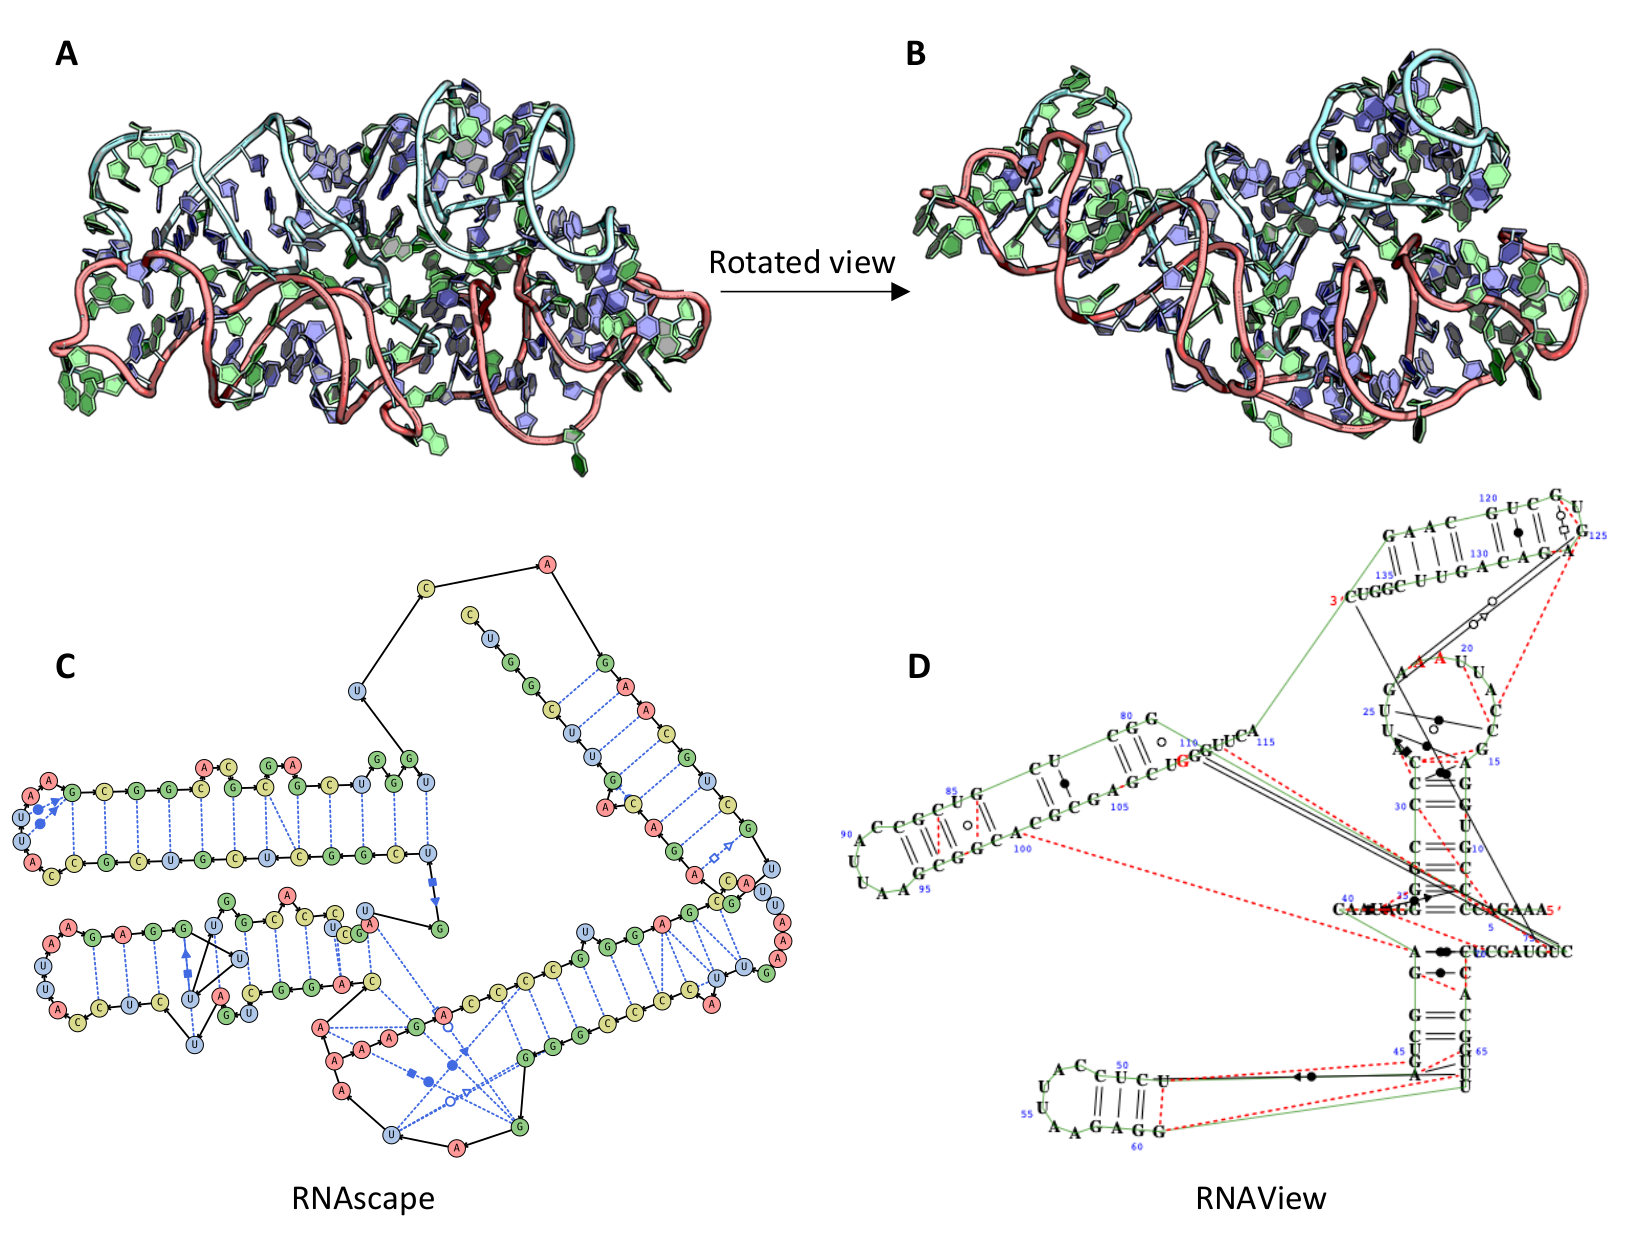
\includegraphics[width=\linewidth]{./rnascapefigs/figureS1.png}
 % archetecture.png: 1149x508 px, 72dpi, 40.53x17.92 cm, bb=0 0 1149 508
    \caption[Tertiary structure aware mapping of the peptidyl transferase center (PTC) of the large ribosomal subunit of Deinococcus radiodurans (PDB ID: 1NKW), also known as proto-ribosome ]{\textbf{Tertiary structure aware mapping of the peptidyl transferase center (PTC) of the large ribosomal subunit of Deinococcus radiodurans (PDB ID: 1NKW), also known as proto-ribosome.} ({\bf A}) Principal axis view of the PTC \citep{Bose2022}. ({\bf B})  Rotated view (approximately 90° about horizontal axis). ({\bf C})  RNAscape visualization of the proto-ribosome in orientation along the principal axis view. ({\bf D})  RNAView \citep{Yang2003} visualization of the proto-ribosome in orientation along the principal axis view. Unlike RNAView, RNAscape captures the semi-symmetric nature of the structure.}
  \label{fig:rnascapeS1}
\end{figure}
\end{center}

\begin{center}
\begin{figure}[H]
  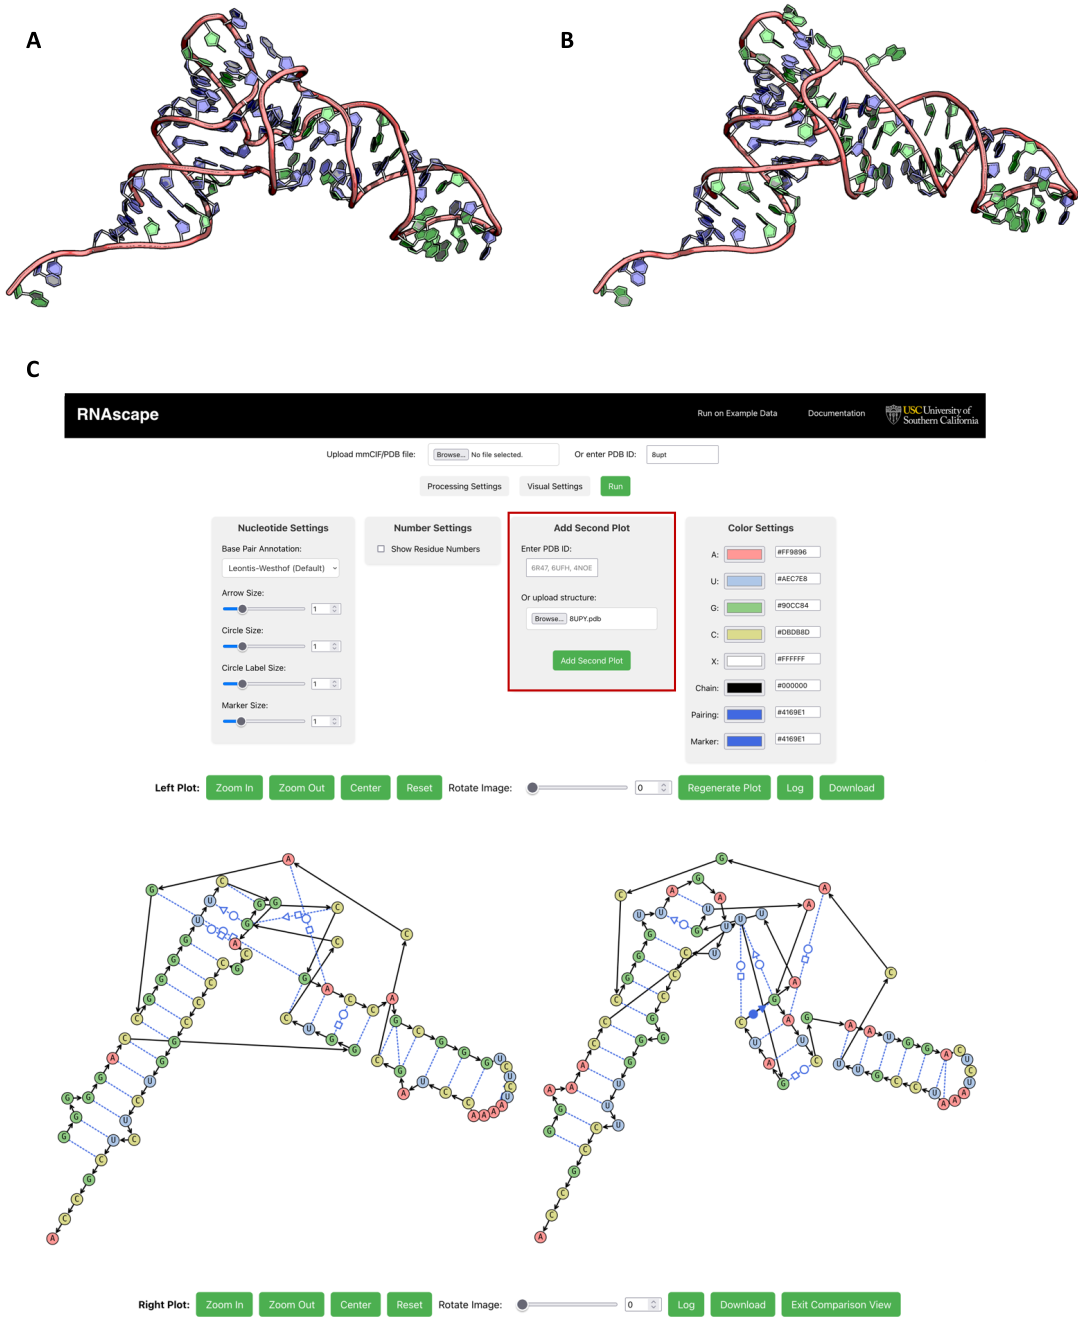
\includegraphics[width=\linewidth]{./rnascapefigs/figureS2.png}
 % archetecture.png: 1149x508 px, 72dpi, 40.53x17.92 cm, bb=0 0 1149 508
    \caption[RNAscape web interface for side-by-side comparison of two structures.]{\textbf{RNAscape web interface for side-by-side comparison of two structures.} ({\bf A}) 3D structure of PDB ID: 8UPT and ({\bf B}) 3D structure of PDB ID: 8UPY. ({\bf C}) After running RNAscape on one structure (in this example, PDB ID: 8UPT \citep{Krahn2024}, a user can upload a second plot for side-by-side comparison (in this example, PDB ID: 8UPY \citep{Krahn2024}. Both plots have separate transformation controls which can be used to orient and compare them.}
  \label{fig:rnascapeS2}
\end{figure}
\end{center}

\begin{center}
\begin{figure}[H]
  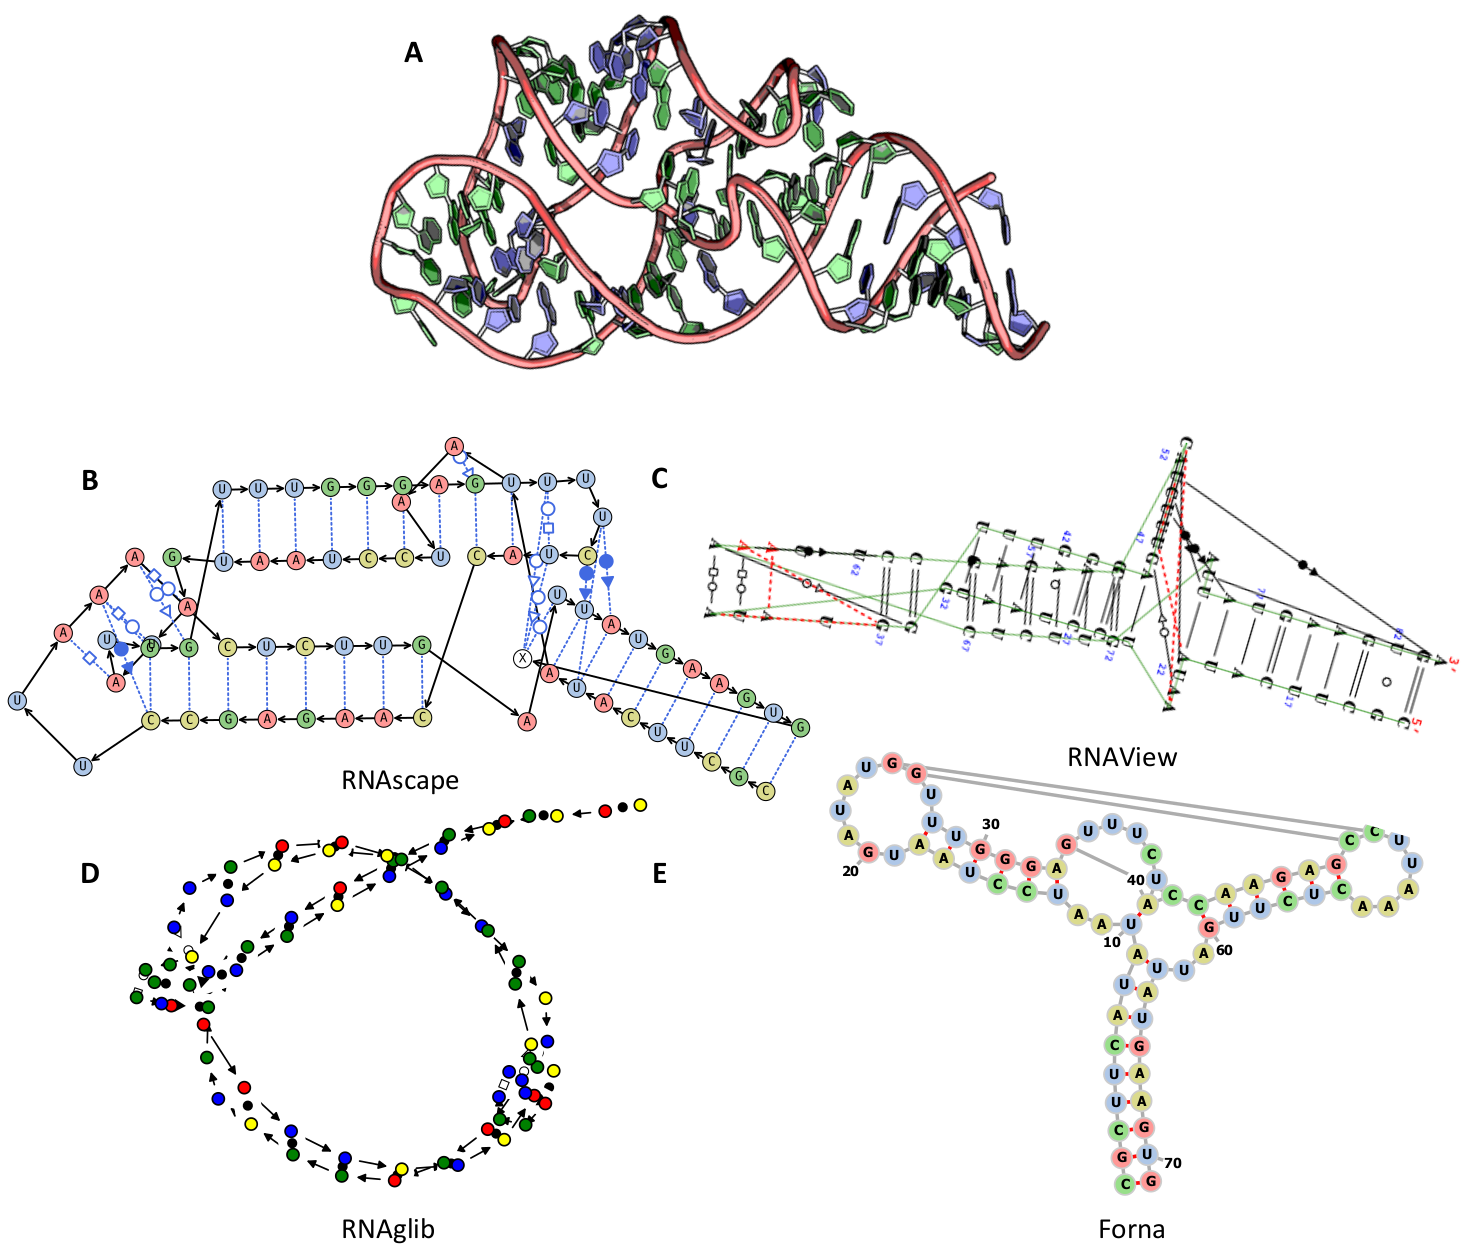
\includegraphics[width=\linewidth]{./rnascapefigs/figureS3.png}
 % archetecture.png: 1149x508 px, 72dpi, 40.53x17.92 cm, bb=0 0 1149 508
    \caption[Visualization of a riboswitch by various methods.]{\textbf{Visualization of a riboswitch by various methods.} ({\bf A}) Riboswitch from Escherichia coli (PDB ID: 1Y26) ({\bf B}) RNAscape visualization. ({\bf C}) RNAView \citep{Yang2003} visualization (rotated to align with the 3D structure.). ({\bf D}) RNAglib \citep{Mallet2022} visualization. ({\bf E}) Seondary structure visualization based on the structure by Forna \citep{Kerpedjiev2015}.}
  \label{fig:rnascapeS3}
\end{figure}
\end{center}
\begin{center}
\begin{figure}[H]
  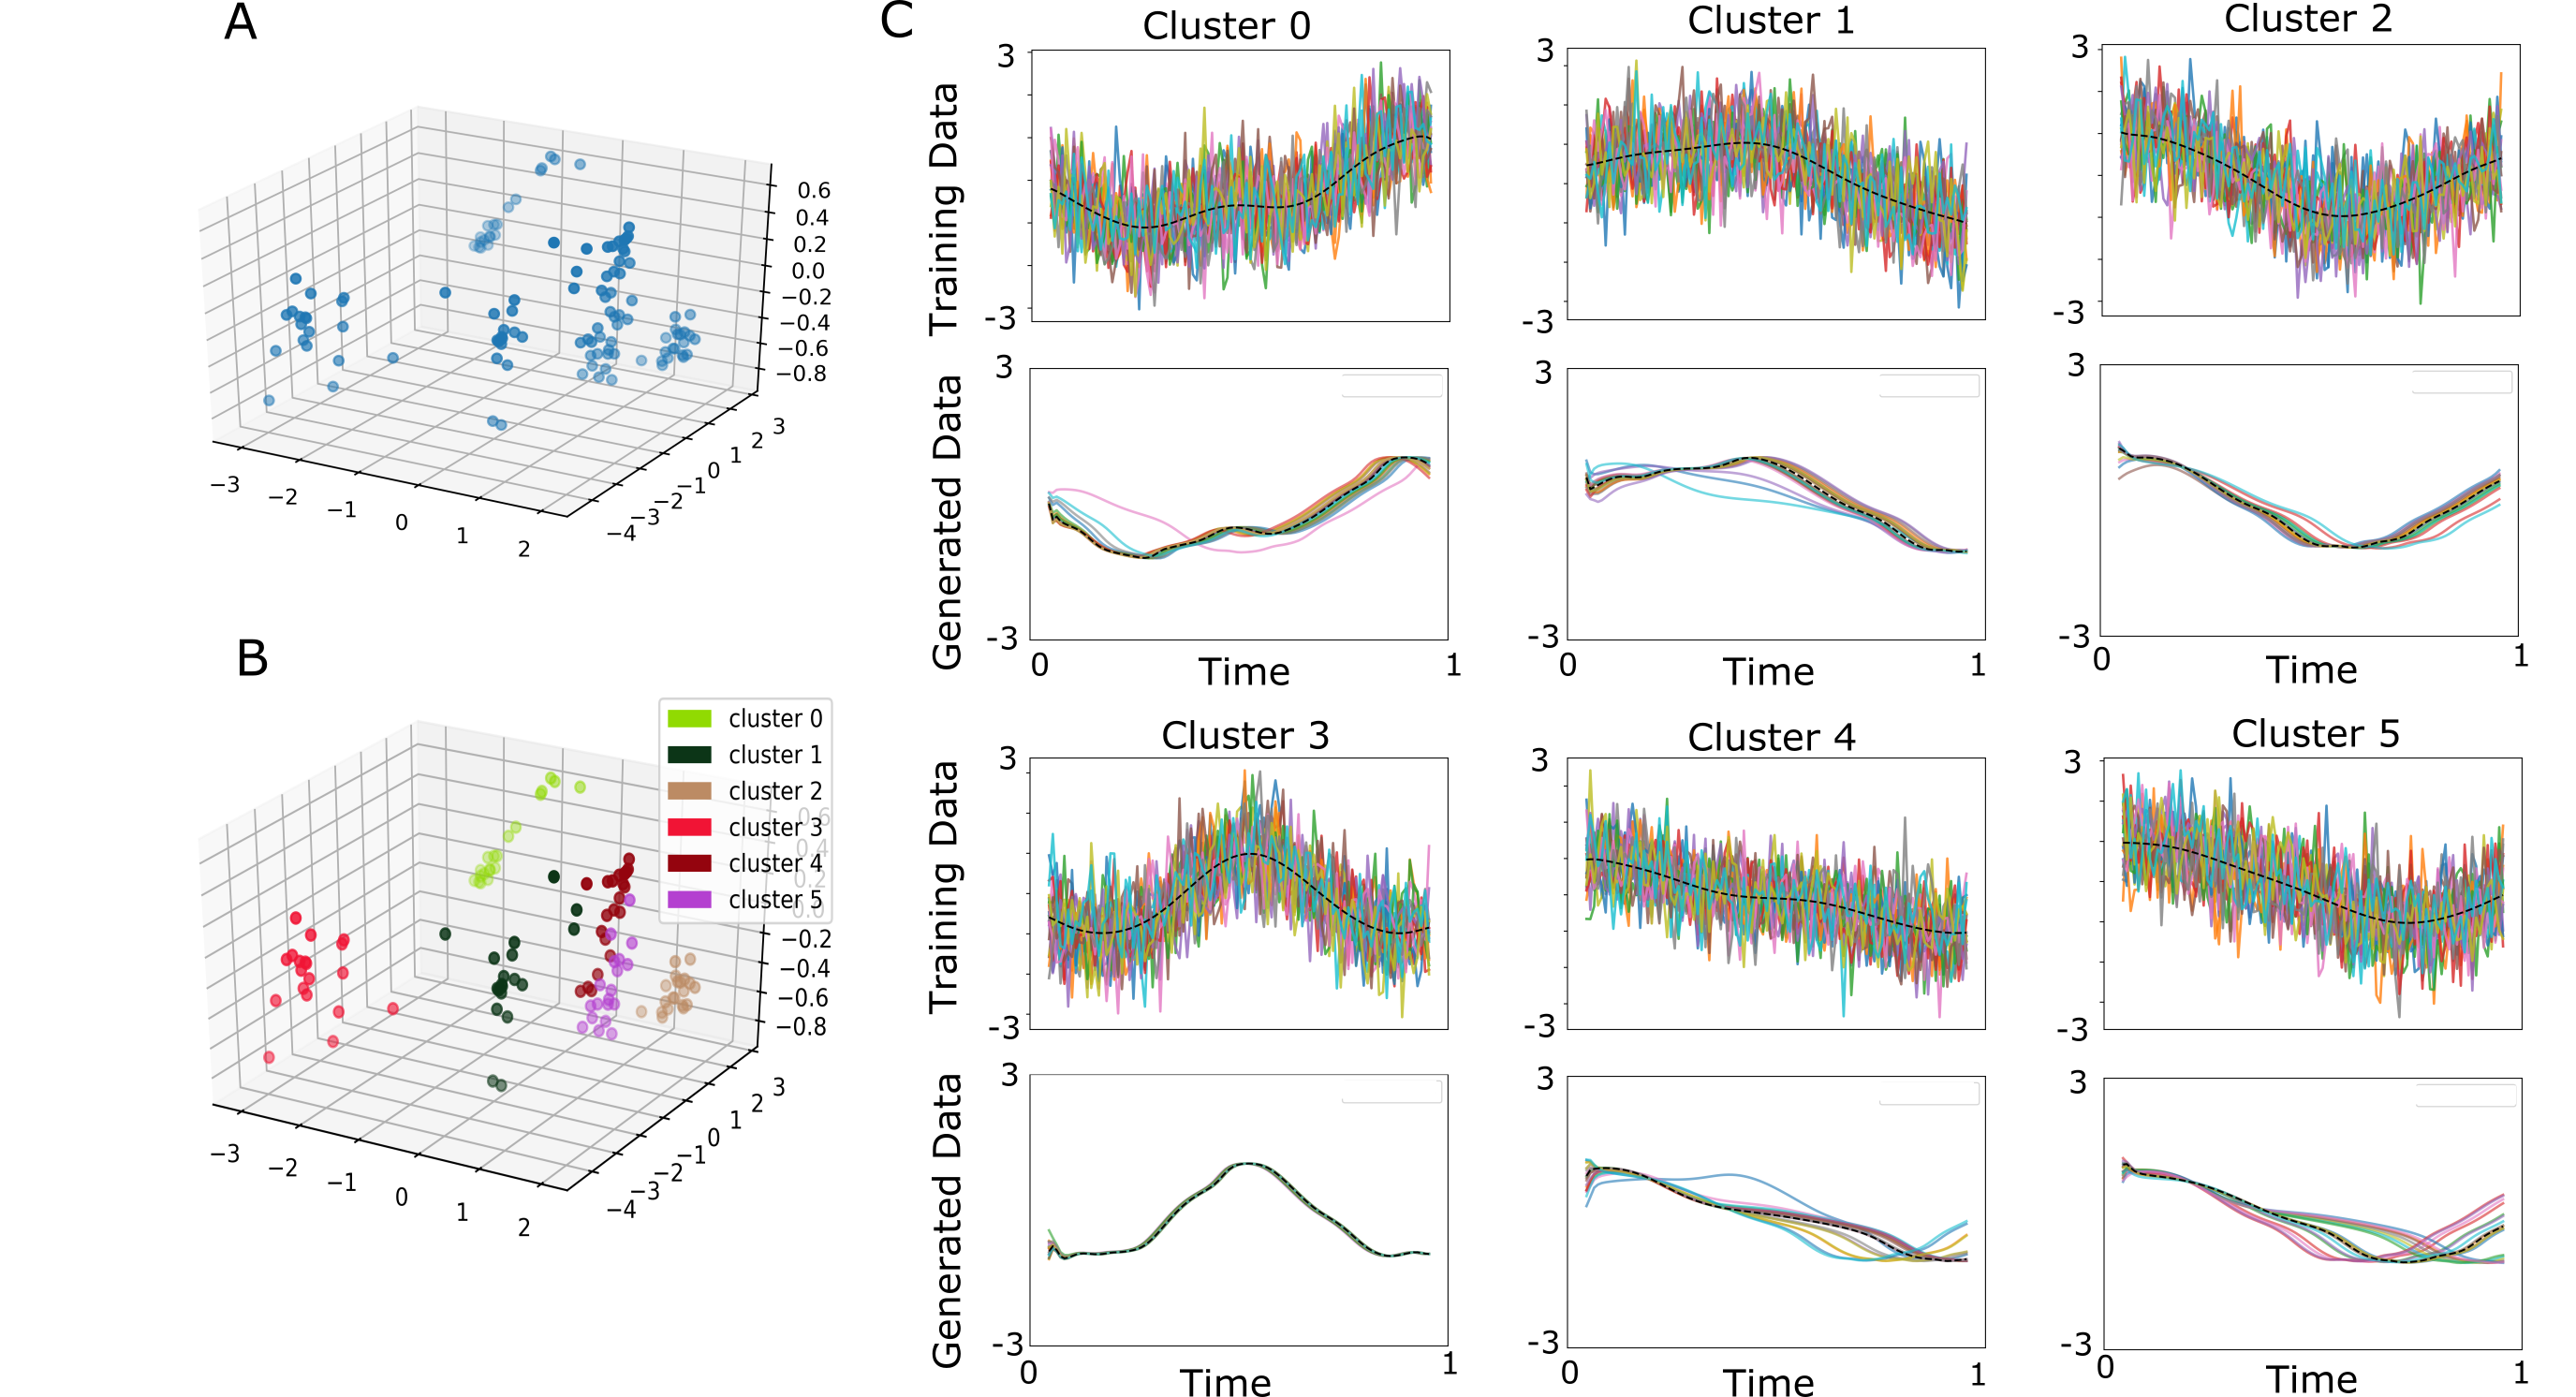
\includegraphics[width=\linewidth]{./figures/noisy_sim.png}
 % archetecture.png: 1149x508 px, 72dpi, 40.53x17.92 cm, bb=0 0 1149 508
    \caption[Demonstration of RVAgene working principle on simulated data with high noise.]{\textbf{Demonstration of RVAgene working principle on simulated data with high noise.} Gaussian noise drawn from $\cN(0,0.7)$ was added to the simulated data to produce a dataset with heavy noise. RVAgene learns the latent space shown in ({\bf A}). ({\bf B}) shows 6 clusters learned by k-means on the learned latent space. ({\bf C}) shows original training data and model generated data from random points in the latent space sampled from $\cN(\mu,0.4\bI)$ around each cluster mean $\mu$ for each of the 6 clusters detected by k-means.}
  \label{fig:figS1}
\end{figure}
\end{center}
\newpage

\begin{center}
\begin{figure}[H]
  \includegraphics[width=\linewidth]{./figures/sl_ESC_r.png}
 % archetecture.png: 1149x508 px, 72dpi, 40.53x17.92 cm, bb=0 0 1149 508
    \caption[Characterization of gene dynamics by linear fit using Pearson correlation coefficient for 5 sample genes in the ESC differentiation dataset]{Characterization of gene dynamics by linear fit using Pearson correlation coefficient for 5 sample genes in the ESC differentiation dataset  \citep{Klein2015}. Blue lines represents original data and orange lines represents linear fits. The Pearson correlation coefficient $r$ is given for each plot.}
  \label{fig:figS2}
\end{figure}
\end{center}
\newpage

\begin{center}
\centering
\begin{figure}[H]
  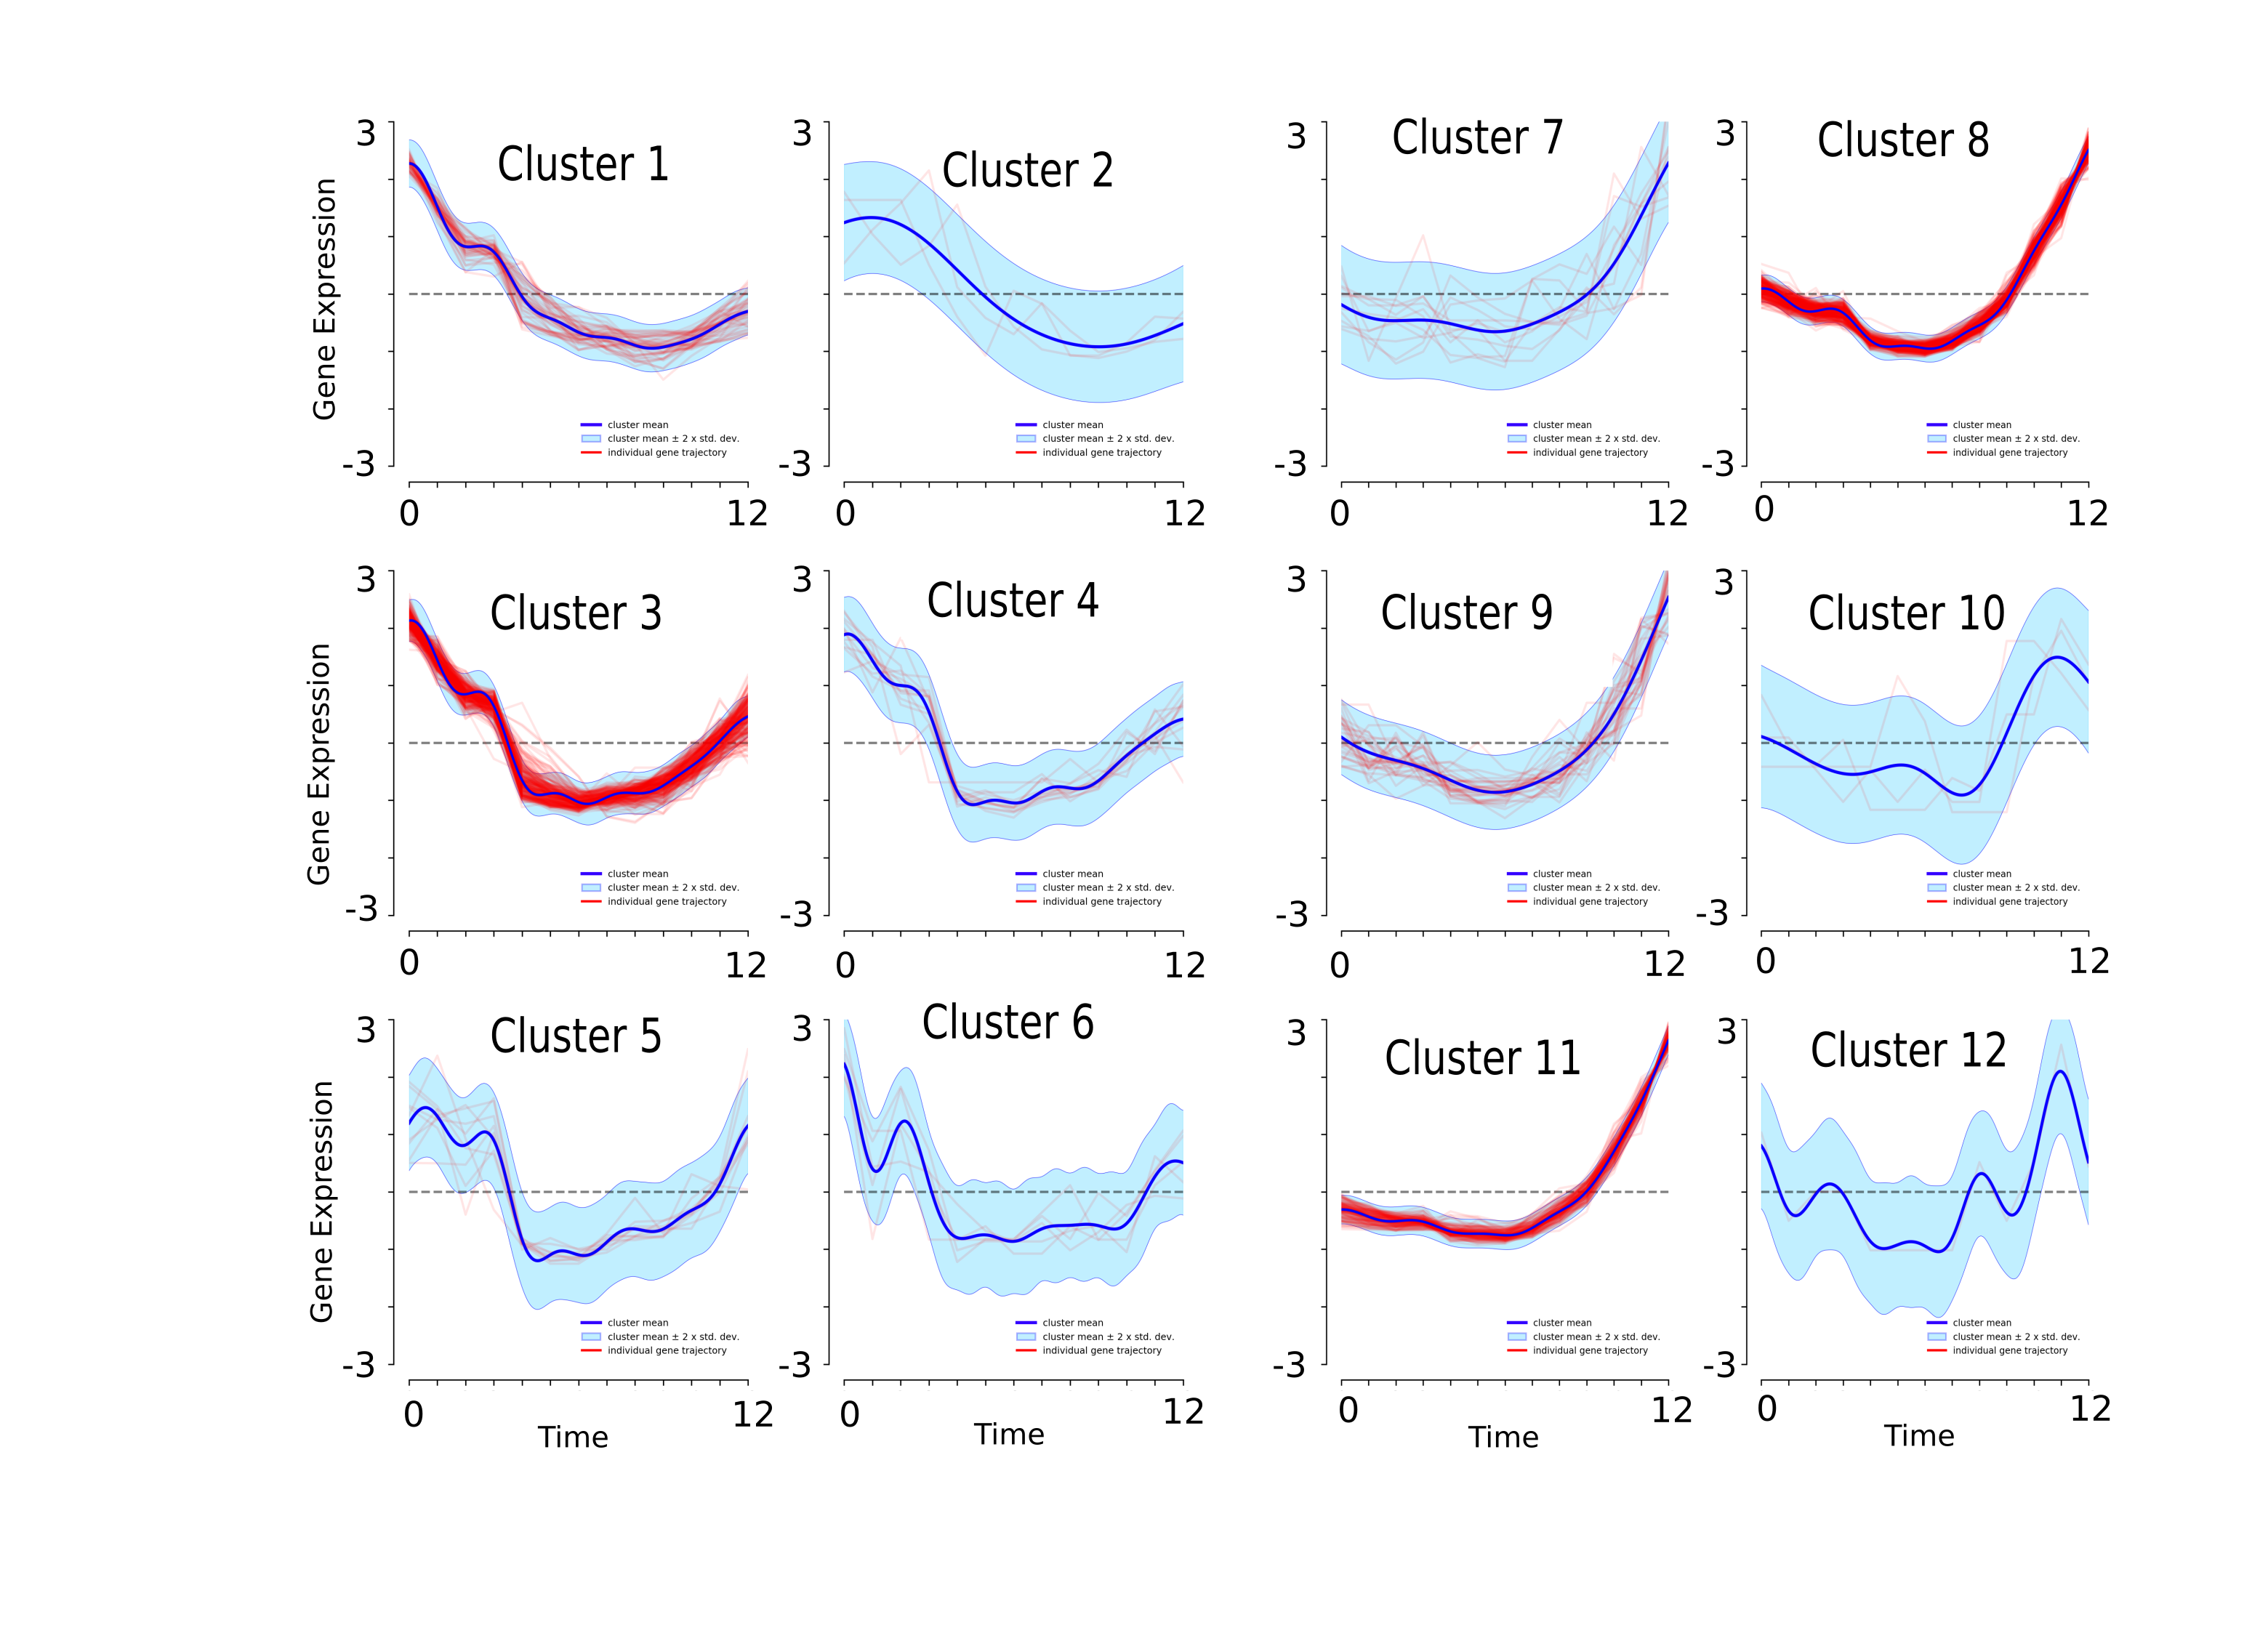
\includegraphics[width=\linewidth,height=0.4\textheight]{figures/fig4.png}
 % archetecture.png: 1149x508 px, 72dpi, 40.53x17.92 cm, bb=0 0 1149 508
    \caption[Clusters detected by the unsupervised clustering algorithm DPGP for ESC differentiation.]{\textbf{Clusters detected by the unsupervised clustering algorithm DPGP for ESC differentiation.} Clusters detected by DPGP in the ESC differentiation dataset  \citep{Klein2015} with default hyperparameters showing cluster means (black), mean $\pm$ 2 s.d. in (blue) and cluster members (red). }
   \label{fig:figS3}
\end{figure}
\end{center}
\newpage
\begin{center}
\begin{figure}
  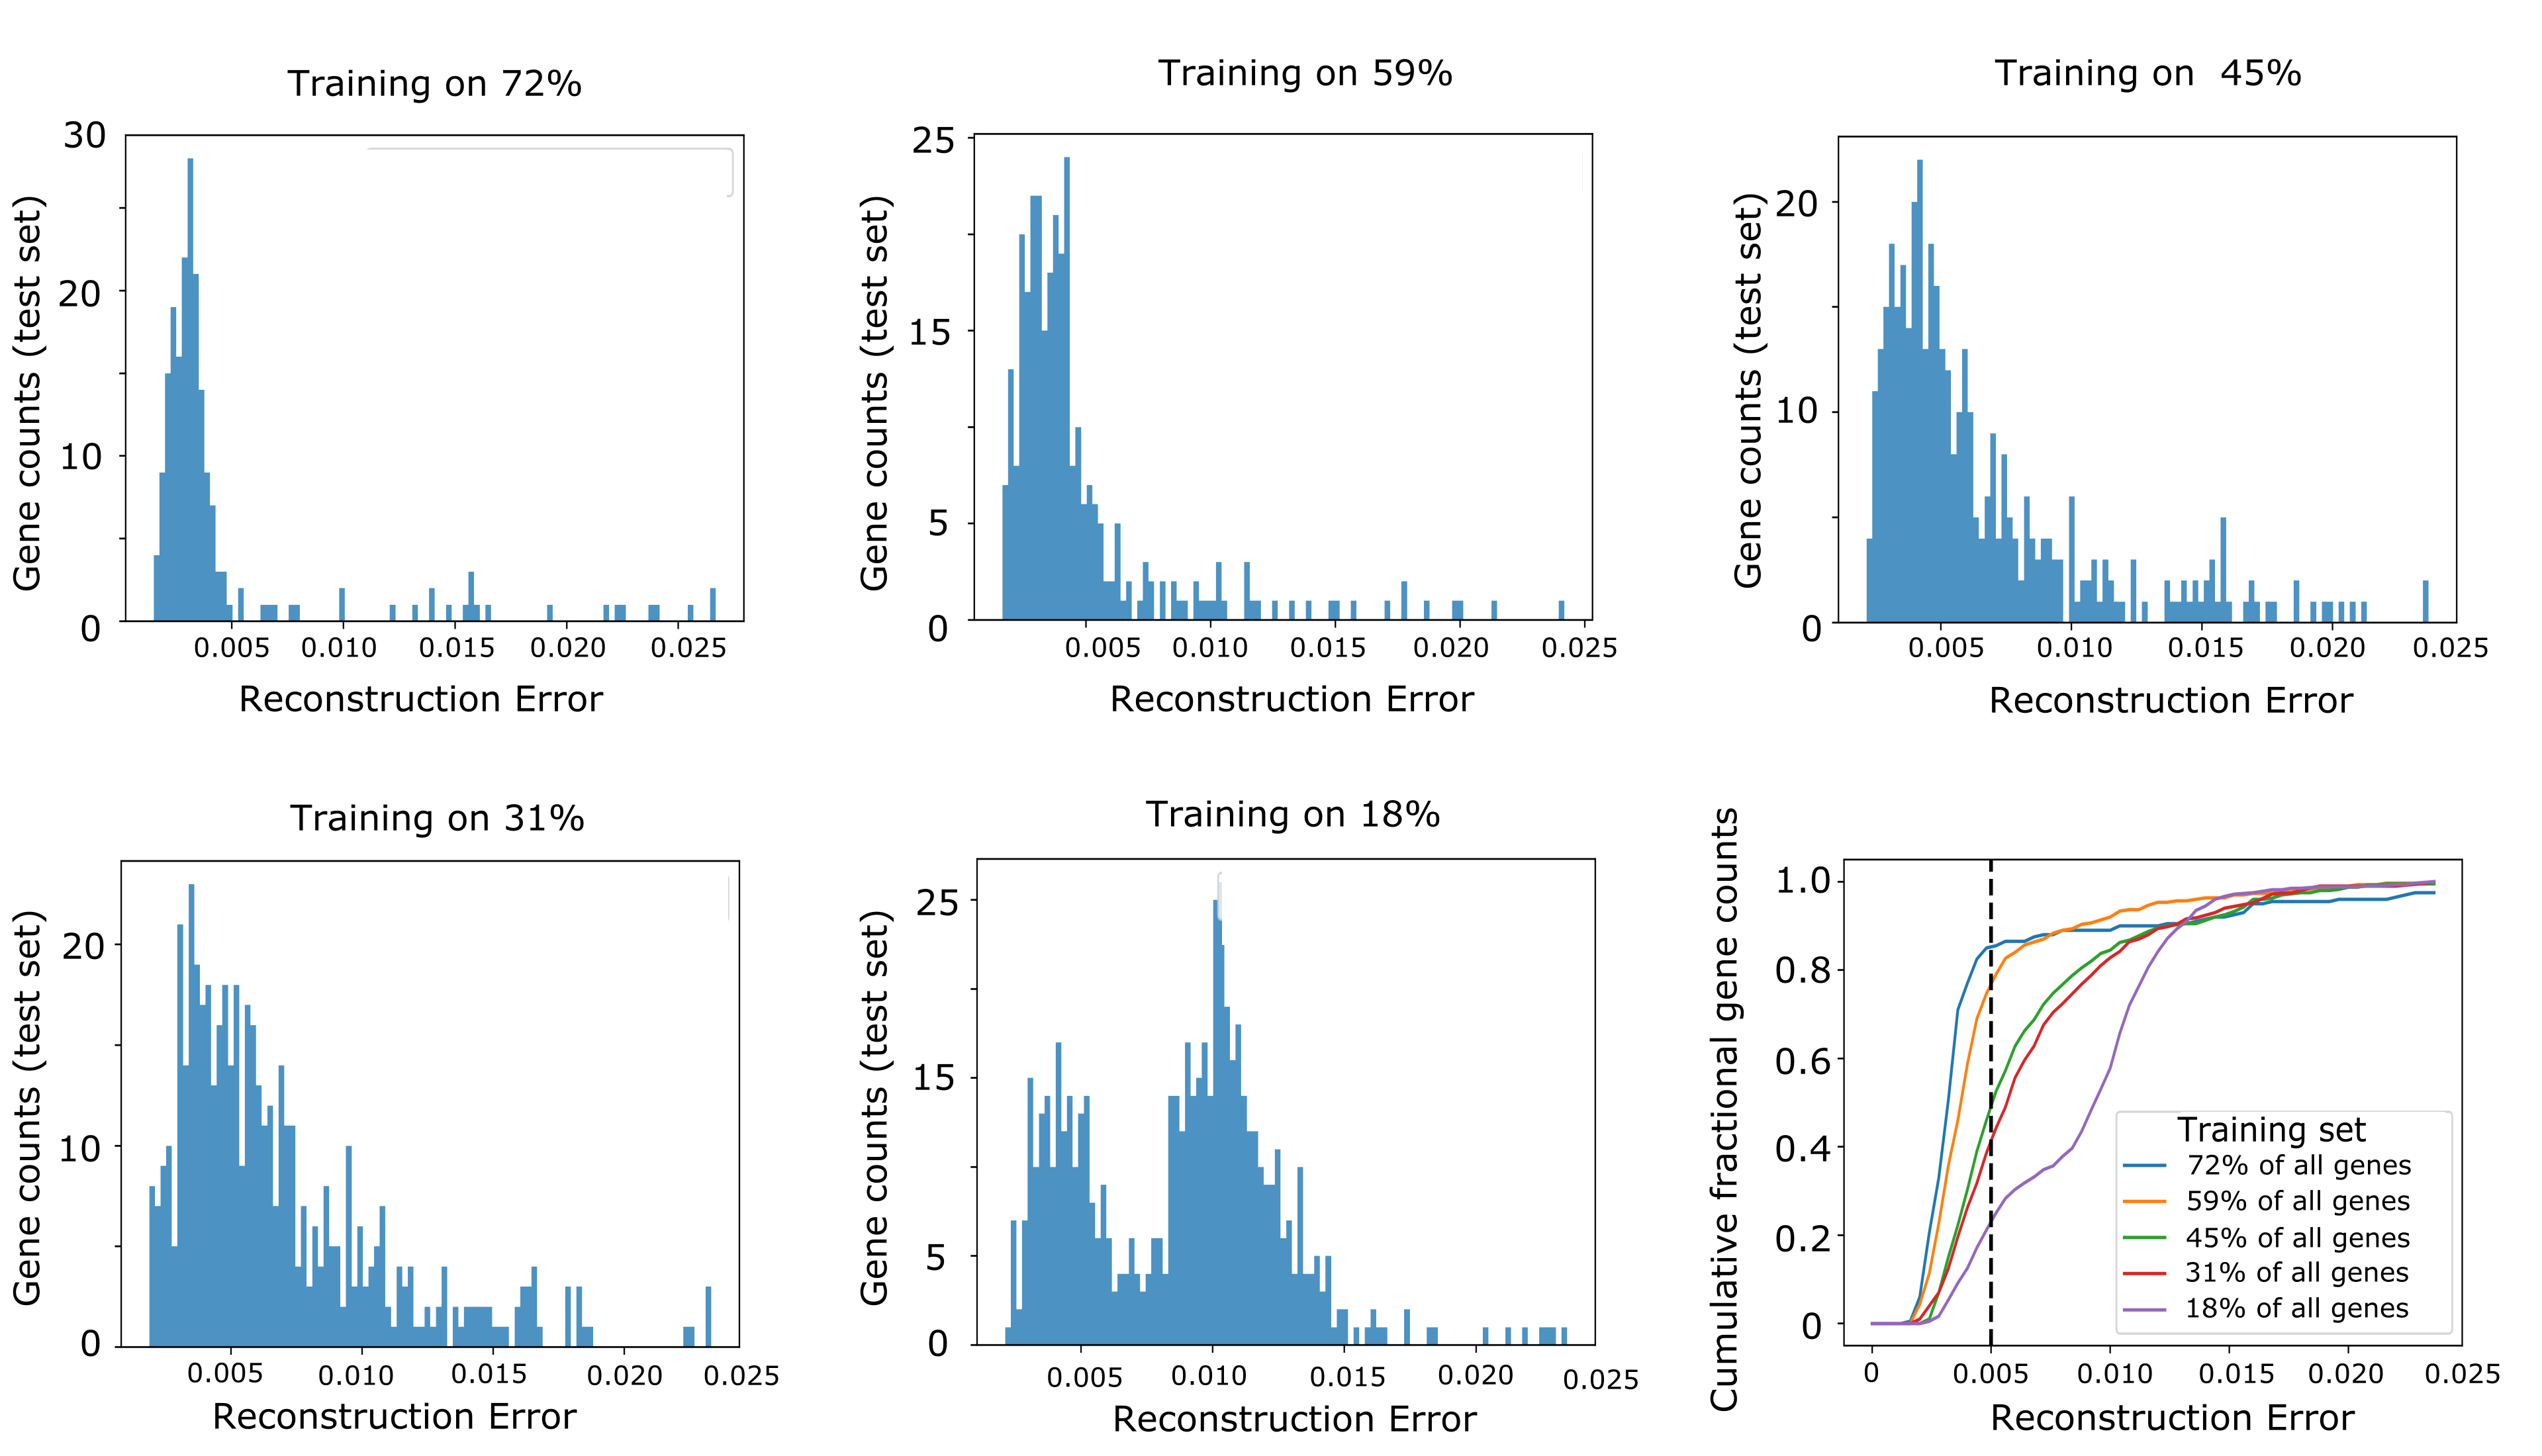
\includegraphics[width=\linewidth]{./figures/supp_varying_test_set_sizes.png}
 % archetecture.png: 1149x508 px, 72dpi, 40.53x17.92 cm, bb=0 0 1149 508
    \caption[Accuracy of RVAgene reconstructions for different train/test group sizes.]{{\bf Accuracy of RVAgene reconstructions for different train/test group sizes.} Distributions of reconstruction errors on randomly sampled sets of test genes, where the full data were split into test groups of: 200 genes (train on 72\%), 300 genes (train on 59\%), 400 genes (train on 45\%), 500 genes (train on 31\%), and 600 genes (train on 18\%). Cumulative fractional distribution of reconstruction errors (cumulative count/test set size) for all groups.}
  \label{fig:figS4}
\end{figure}
\end{center}
\newpage

\begin{center}
\begin{figure}[H]
  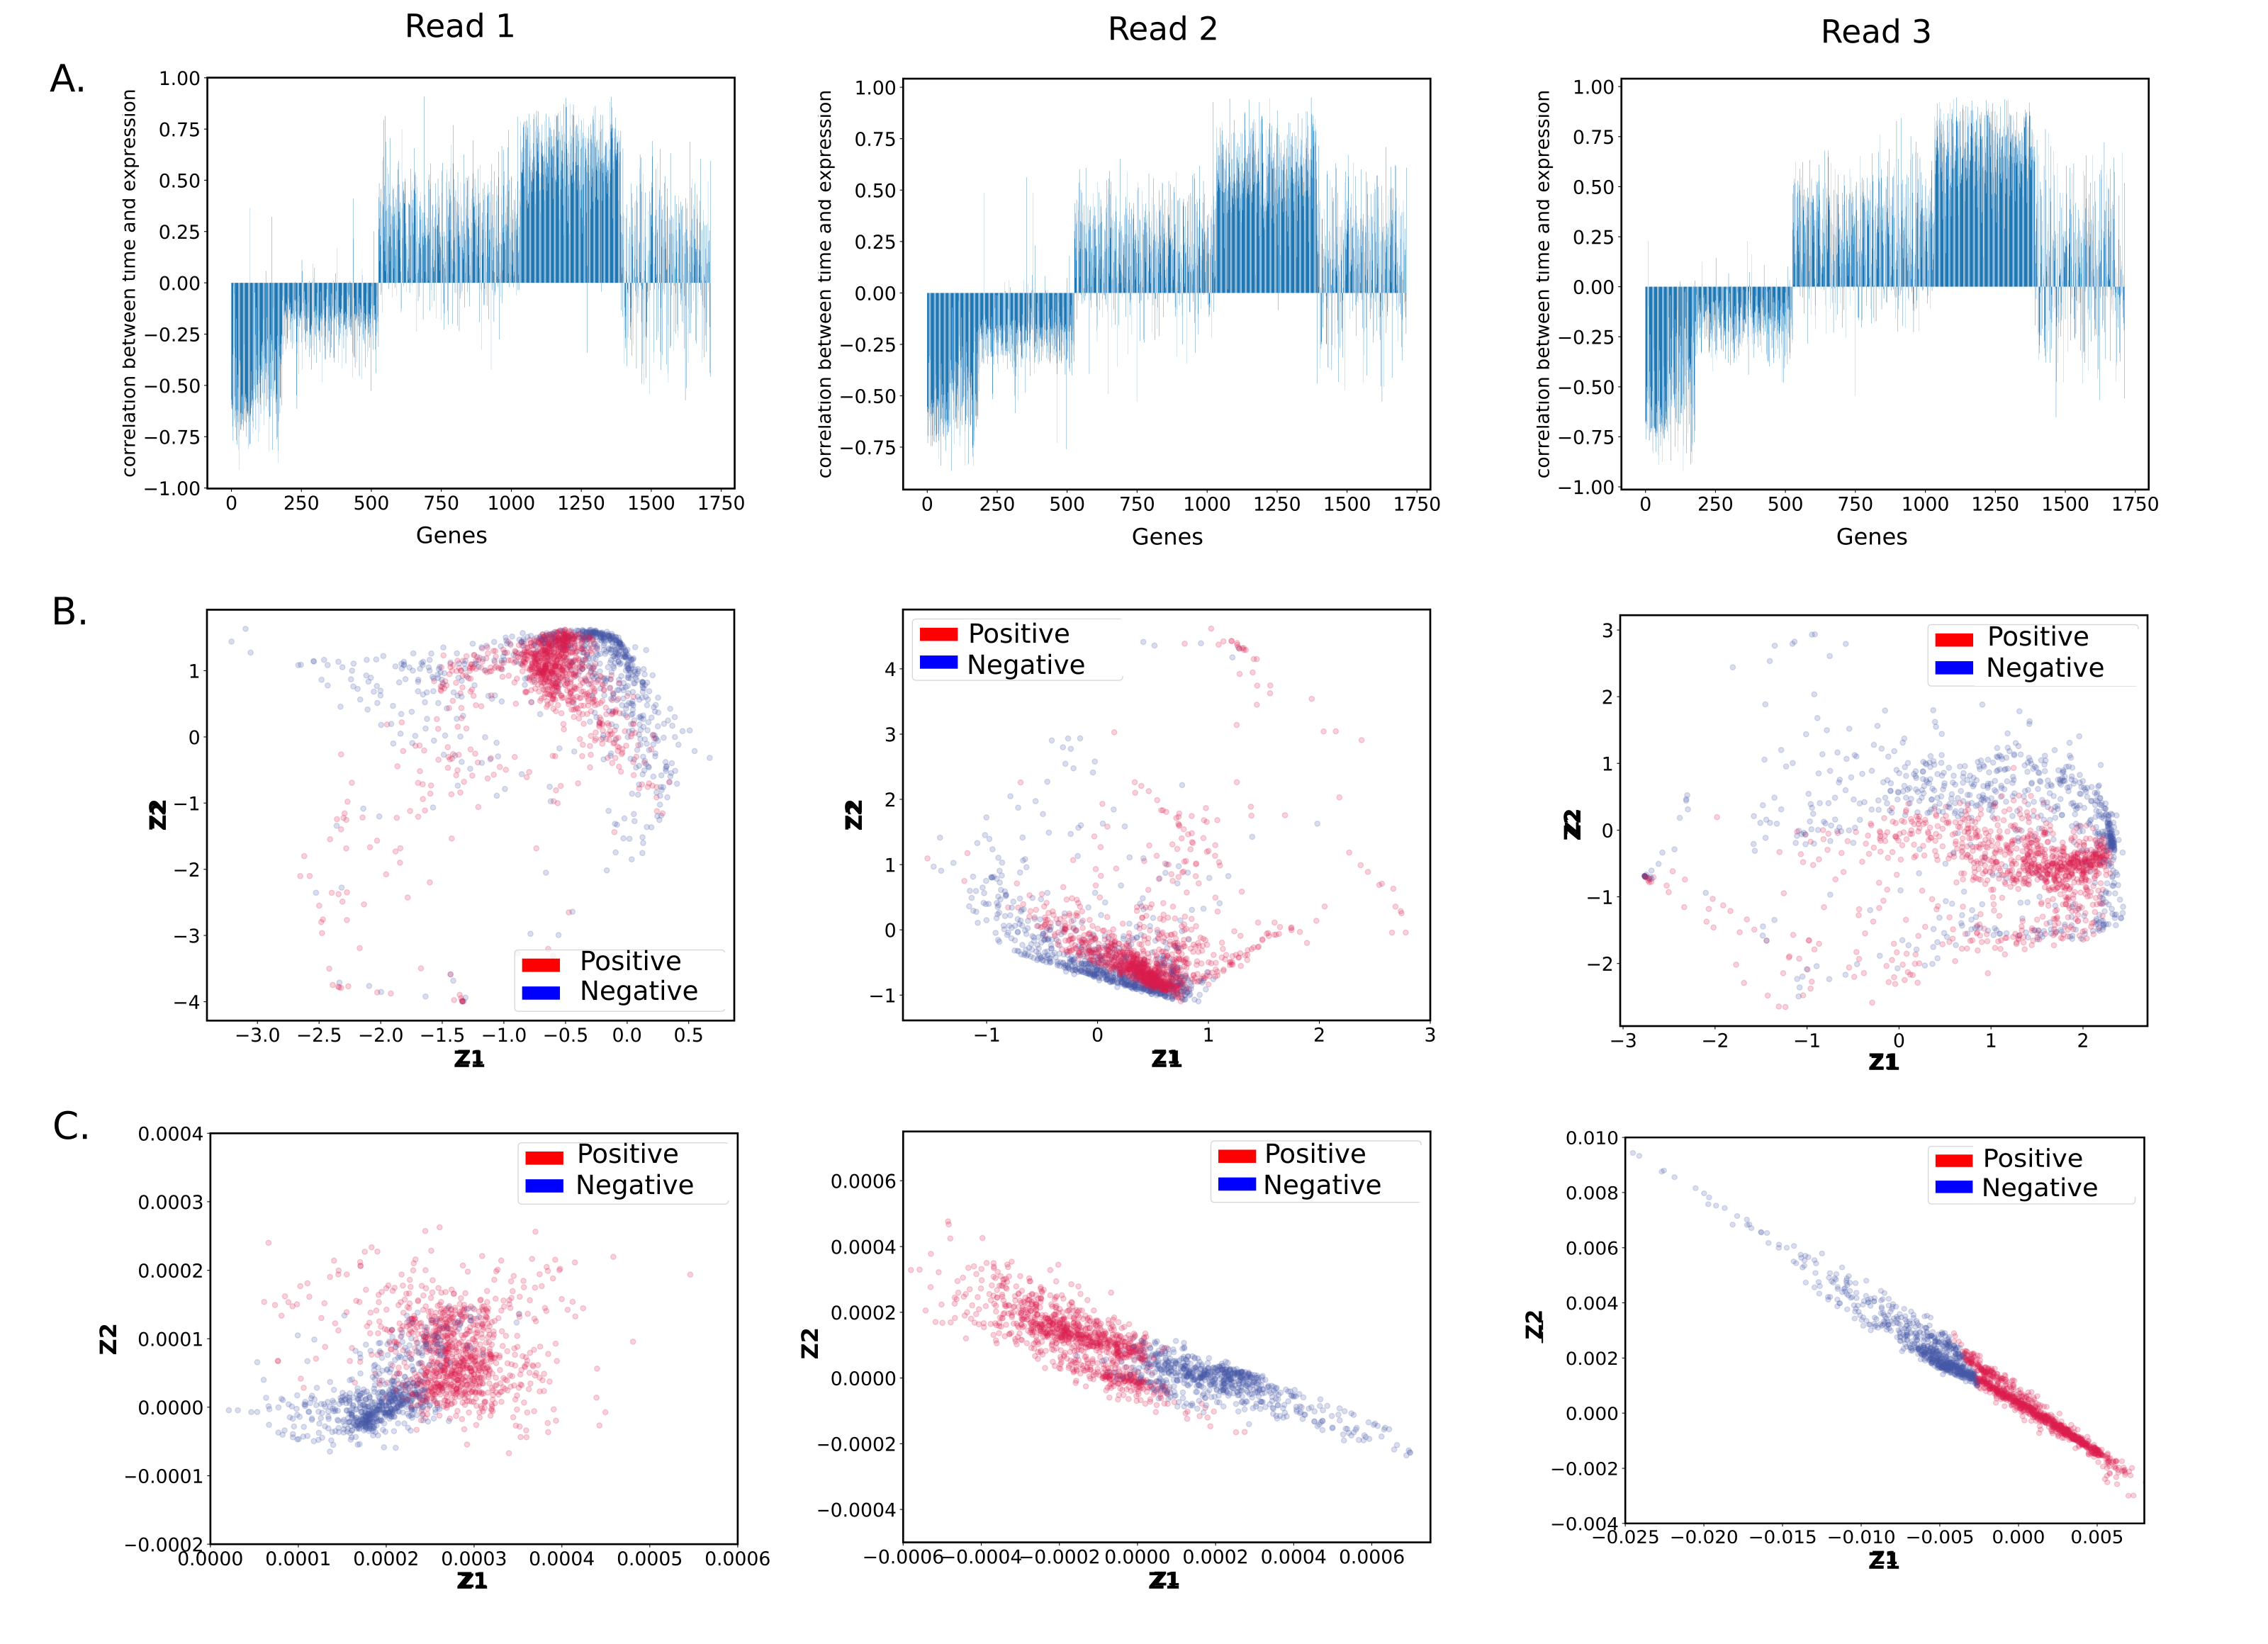
\includegraphics[width = \linewidth]{figures/fig8.png}
 % archetecture.png: 1149x508 px, 72dpi, 40.53x17.92 cm, bb=0 0 1149 508
    \caption[Modeling response to kidney injury and analysis of linear fits.]{\textbf{Modeling response to kidney injury and analysis of linear fits.}
    ({\bf A}) Pearson correlation coefficients between gene expression and time for each differentially expressed gene in the kidney injury dataset for each of the 3 replicates \citep{liu2017molecular}. ({\bf B}) RVAgene latent space representation of fitted model for each replicate; color represents positive or negative correlation coefficients. ({\bf C}) RVAgene latent space representation learnt for the same three replicates as in (B), but where every input gene was normalized  so that its expression sums to 1.}
  \label{fig:figS5}
\end{figure}
\end{center}
\newpage

\begin{center}
\begin{figure}[H]
  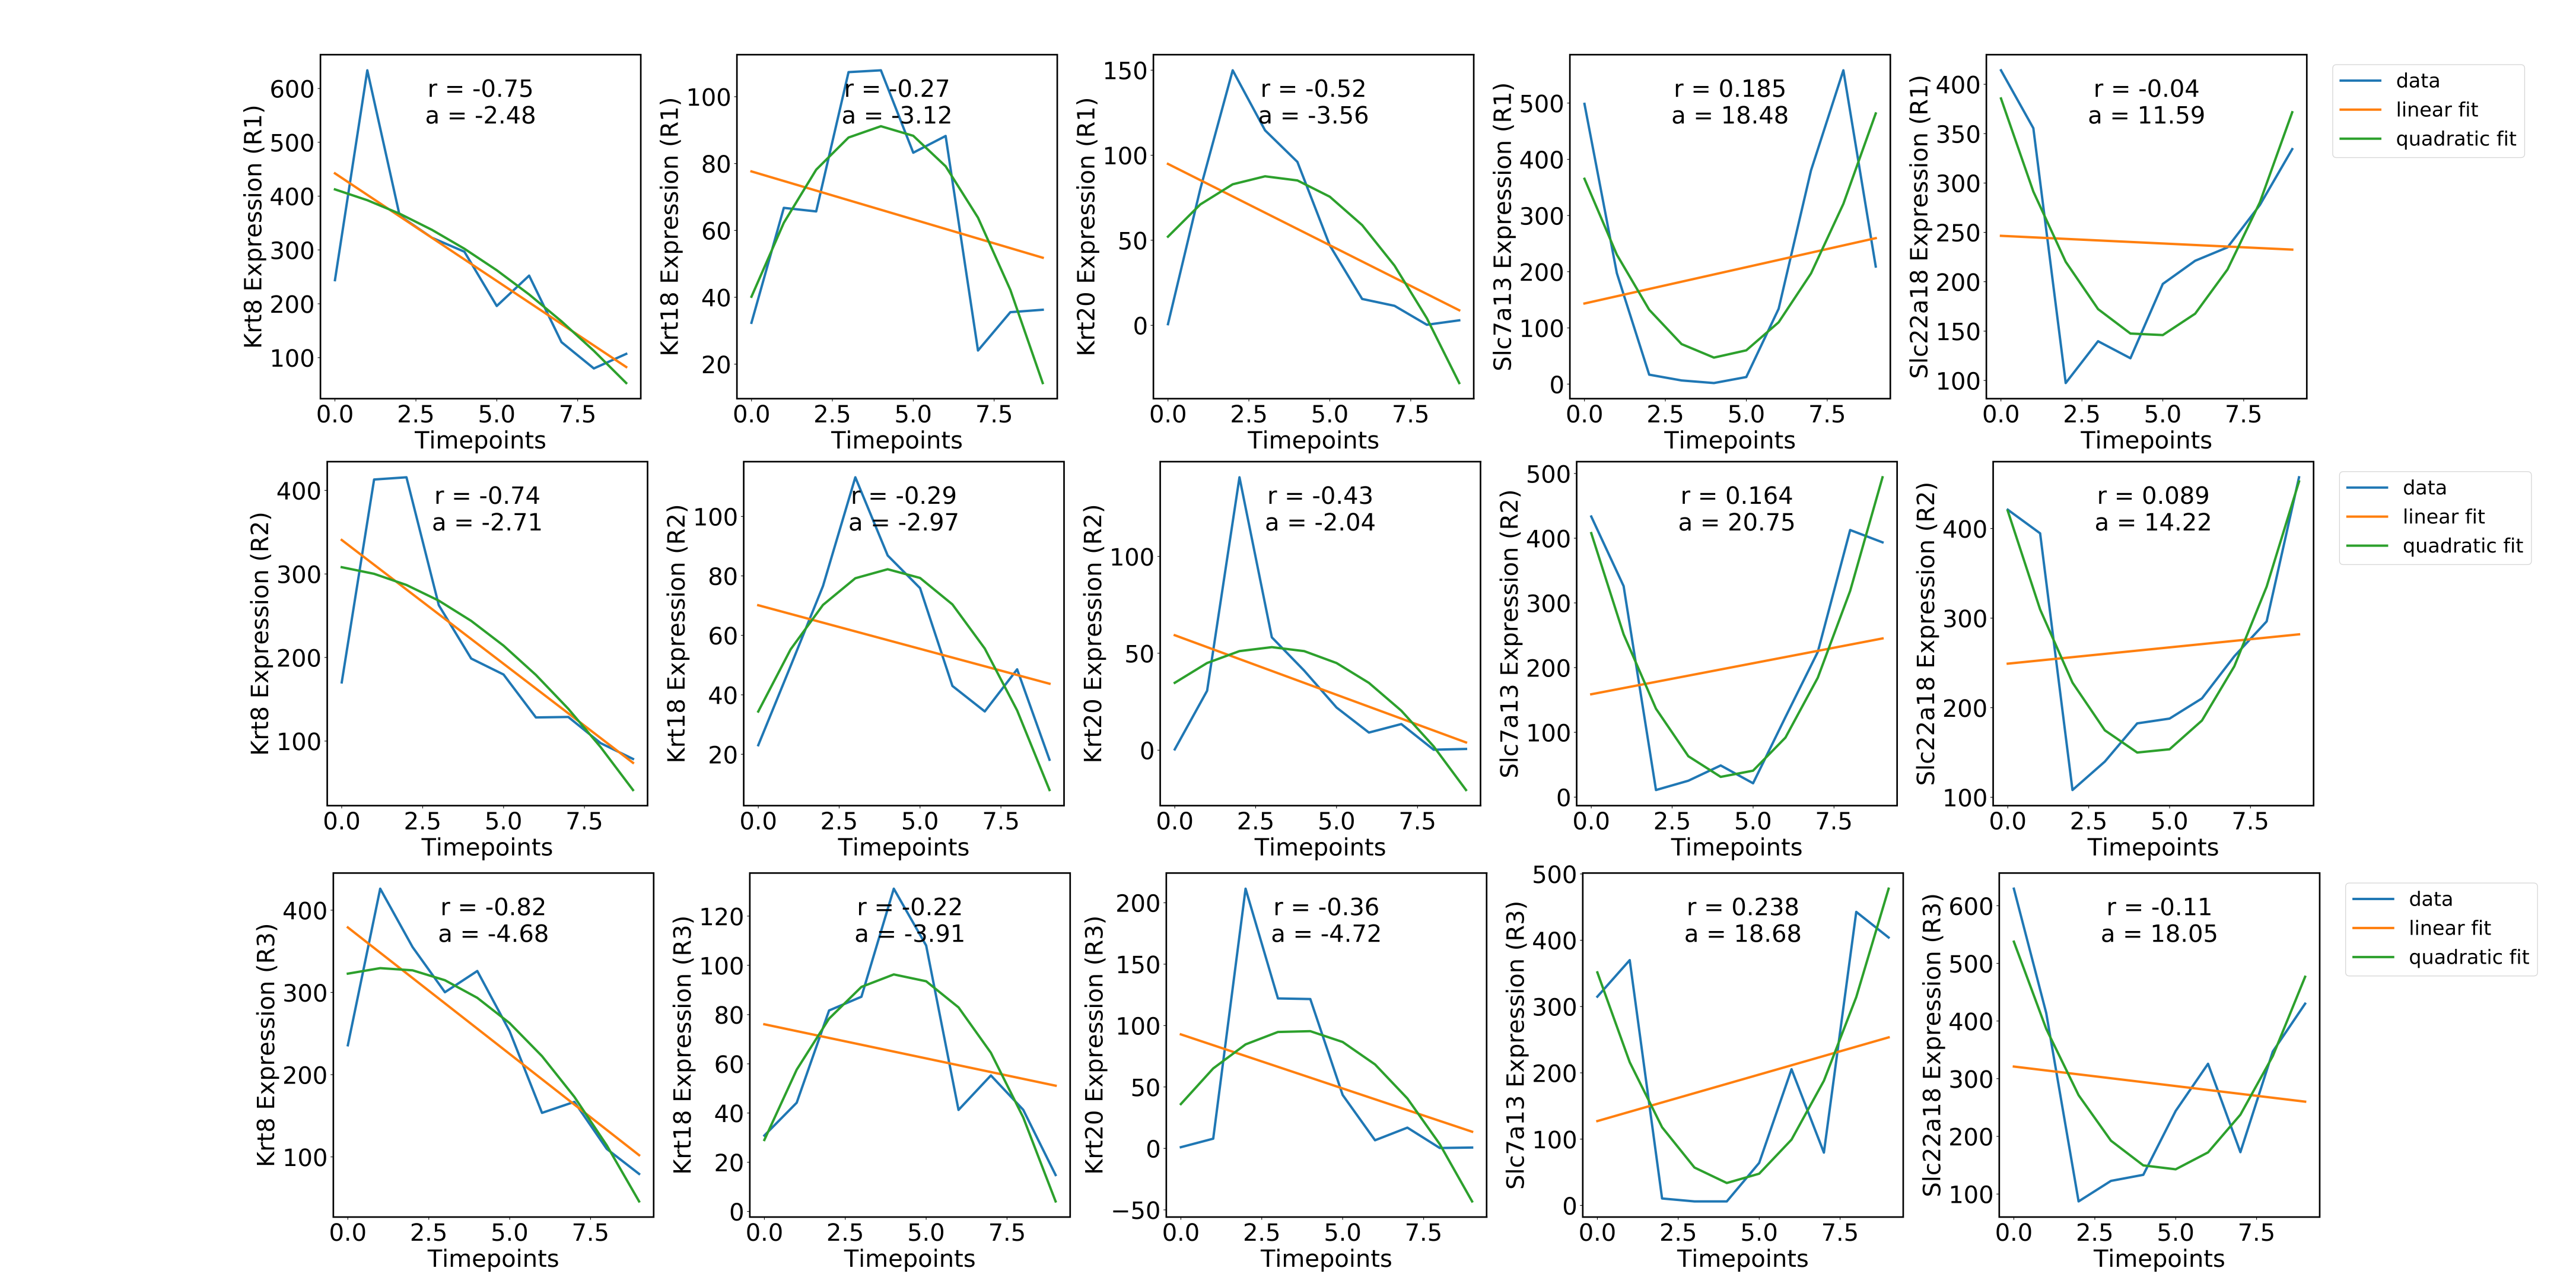
\includegraphics[width=\linewidth]{./figures/sl_JCI_r.png}
 % archetecture.png: 1149x508 px, 72dpi, 40.53x17.92 cm, bb=0 0 1149 508
    \caption[Comparison of linear and quadratic fits to describe gene dynamics in response to kidney injury.]{\textbf{Comparison of linear and quadratic fits to describe gene dynamics in response to kidney injury.}
    For each of the three replicates (R1-R3), five genes are shown, with experimental data (blue), linear fit (orange), and quadratic fit (green). 
    Pearson correlation coefficients, $r$, and quadratic coefficients, $a$ ($x = at^2 + bt + c$), are given for each plot.}
  \label{fig:figS6}
\end{figure}
\end{center}
\newpage

\begin{center}
\begin{figure}[H]
  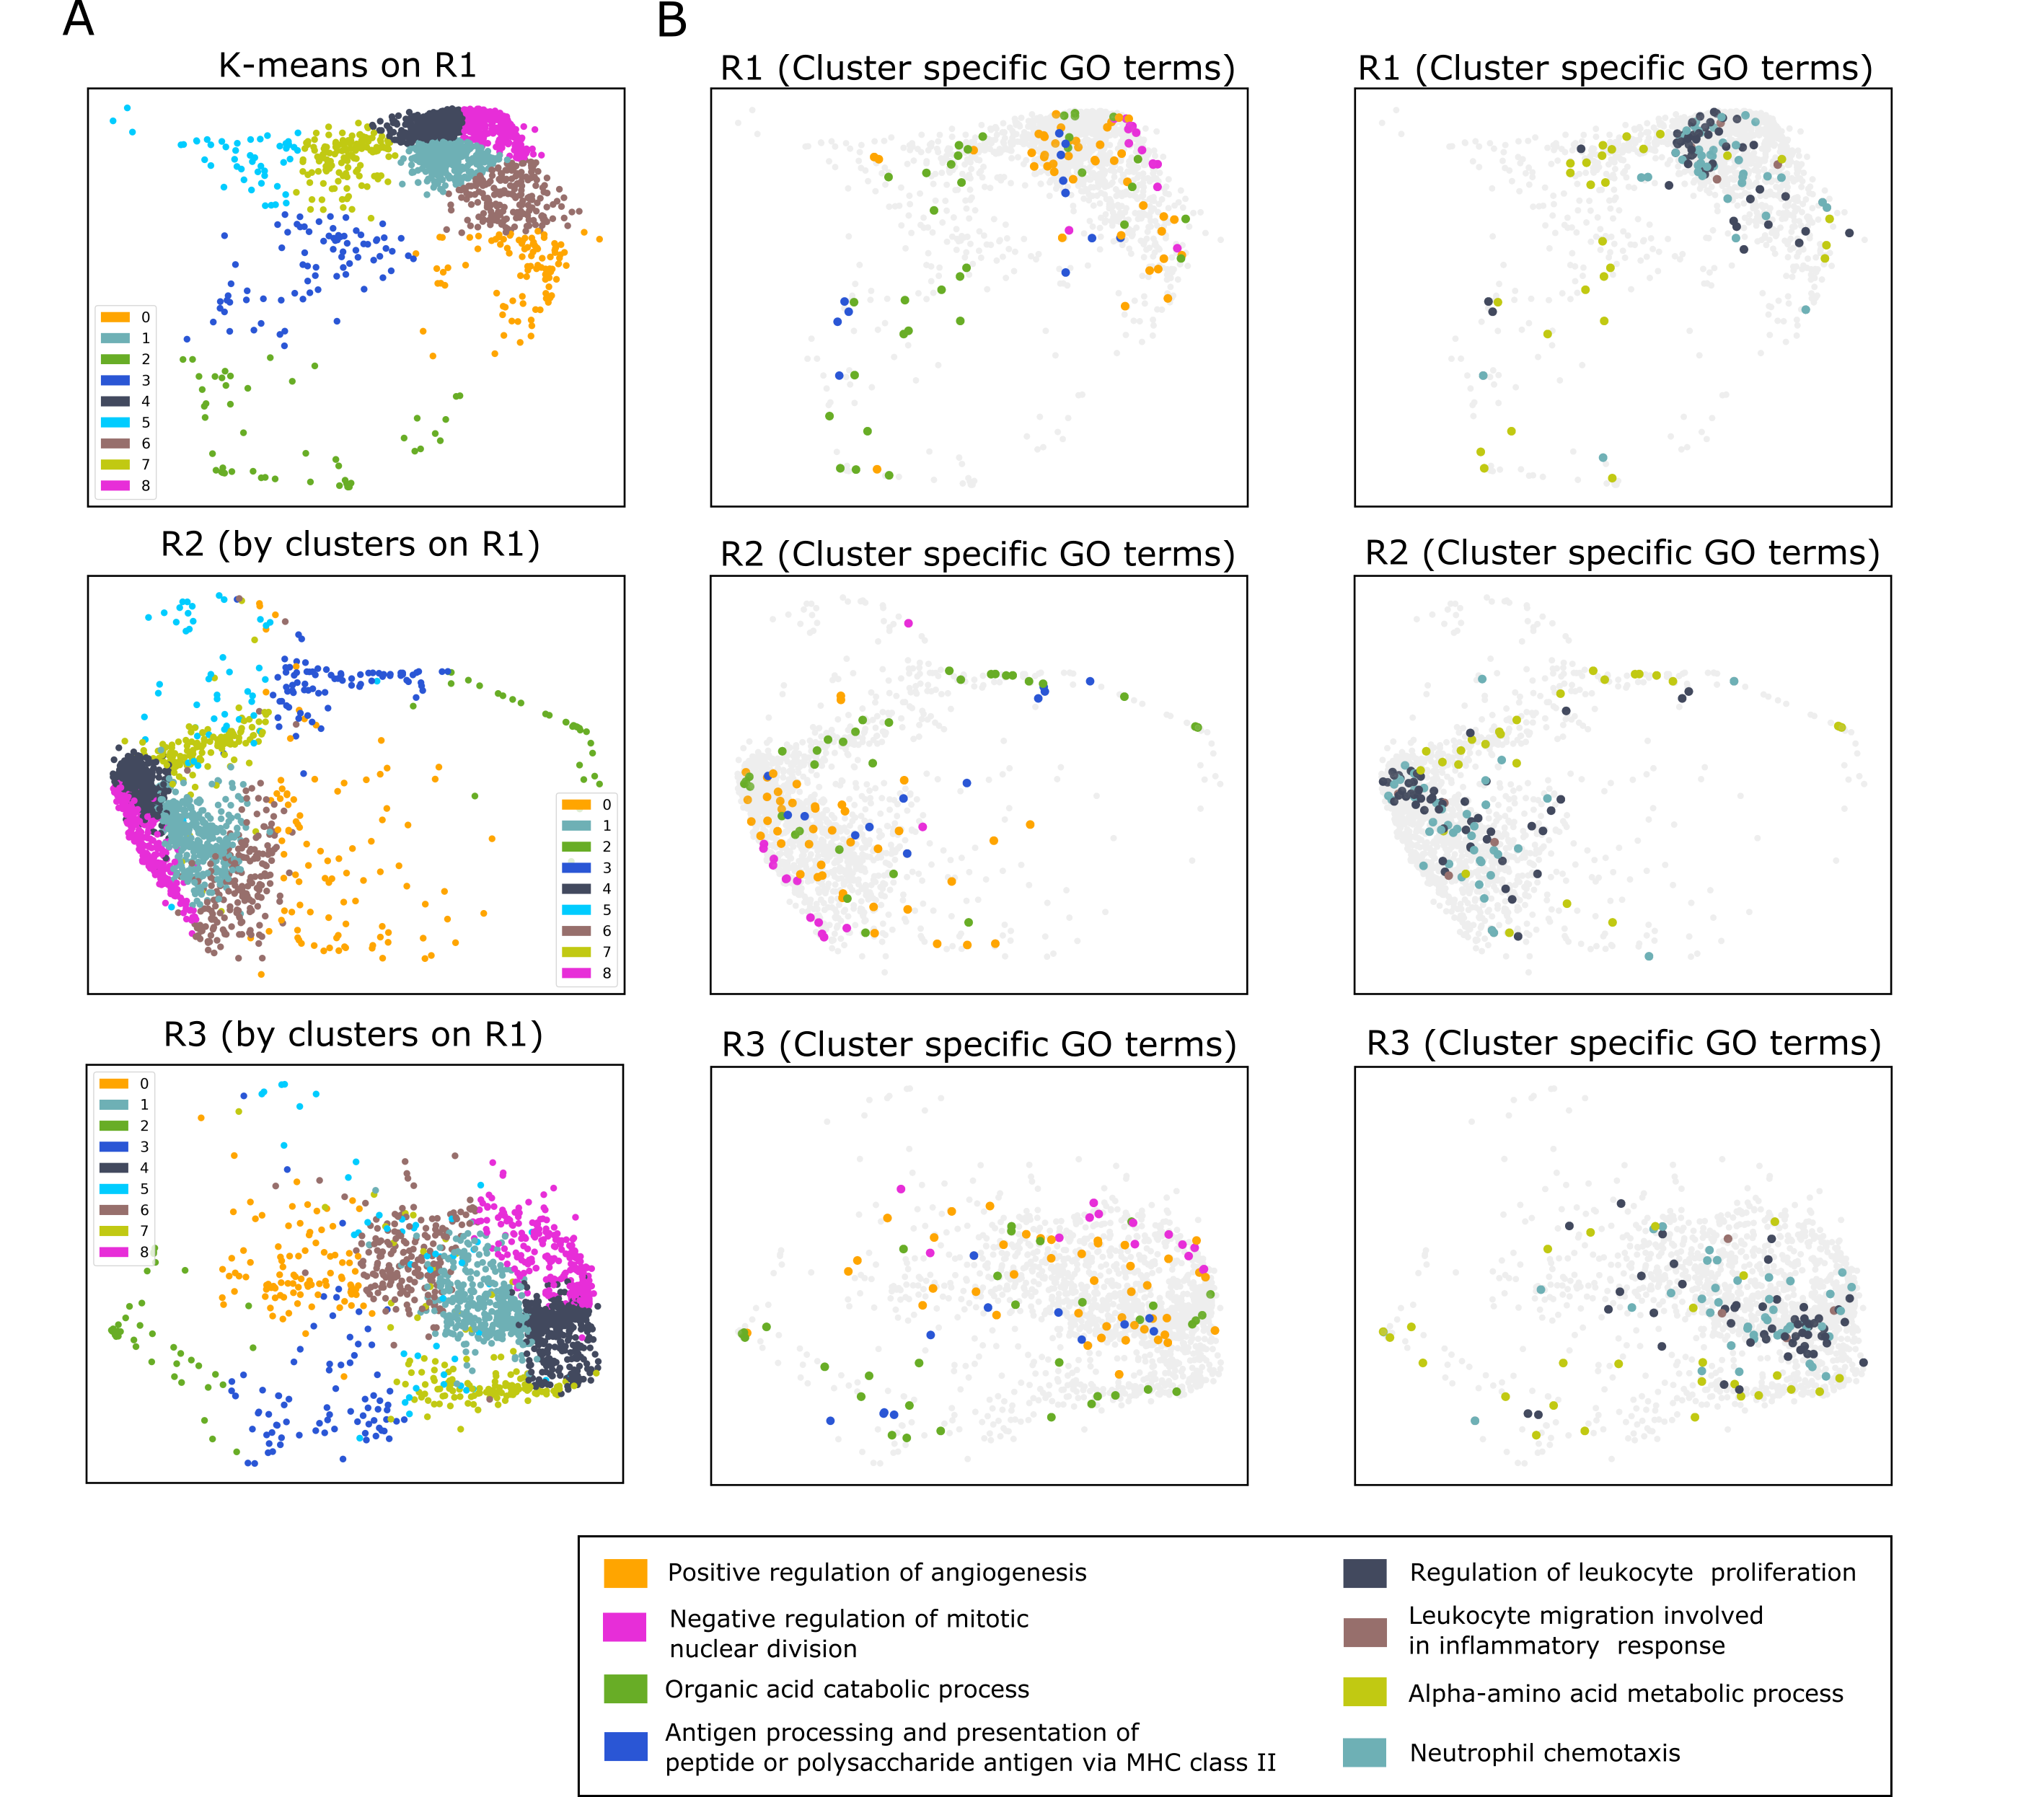
\includegraphics[width=\linewidth]{./figures/supp_go.png}
 % archetecture.png: 1149x508 px, 72dpi, 40.53x17.92 cm, bb=0 0 1149 508
    \caption[Clustering on R1 and cluster specific GO enrichment analysis.]{\textbf{Clustering on R1 and cluster specific GO enrichment analysis.} We performed k-means clustering on latent space learned by RVAgene on R1 with $k=9$. We also show learned latent space on R2 and R3 annotated by the clustering done on R1. All clusters (except cluster 5) appears well preserved. We perform GO analysis for each cluster and select one significant GO term from each cluster (except cluster 5) and show how all genes in the dataset corresponding to each GO term appears on the latent space for all three replicates. }
  \label{fig:figS8}
\end{figure}
\end{center}
\newpage

\begin{center}
\begin{figure}[H]
  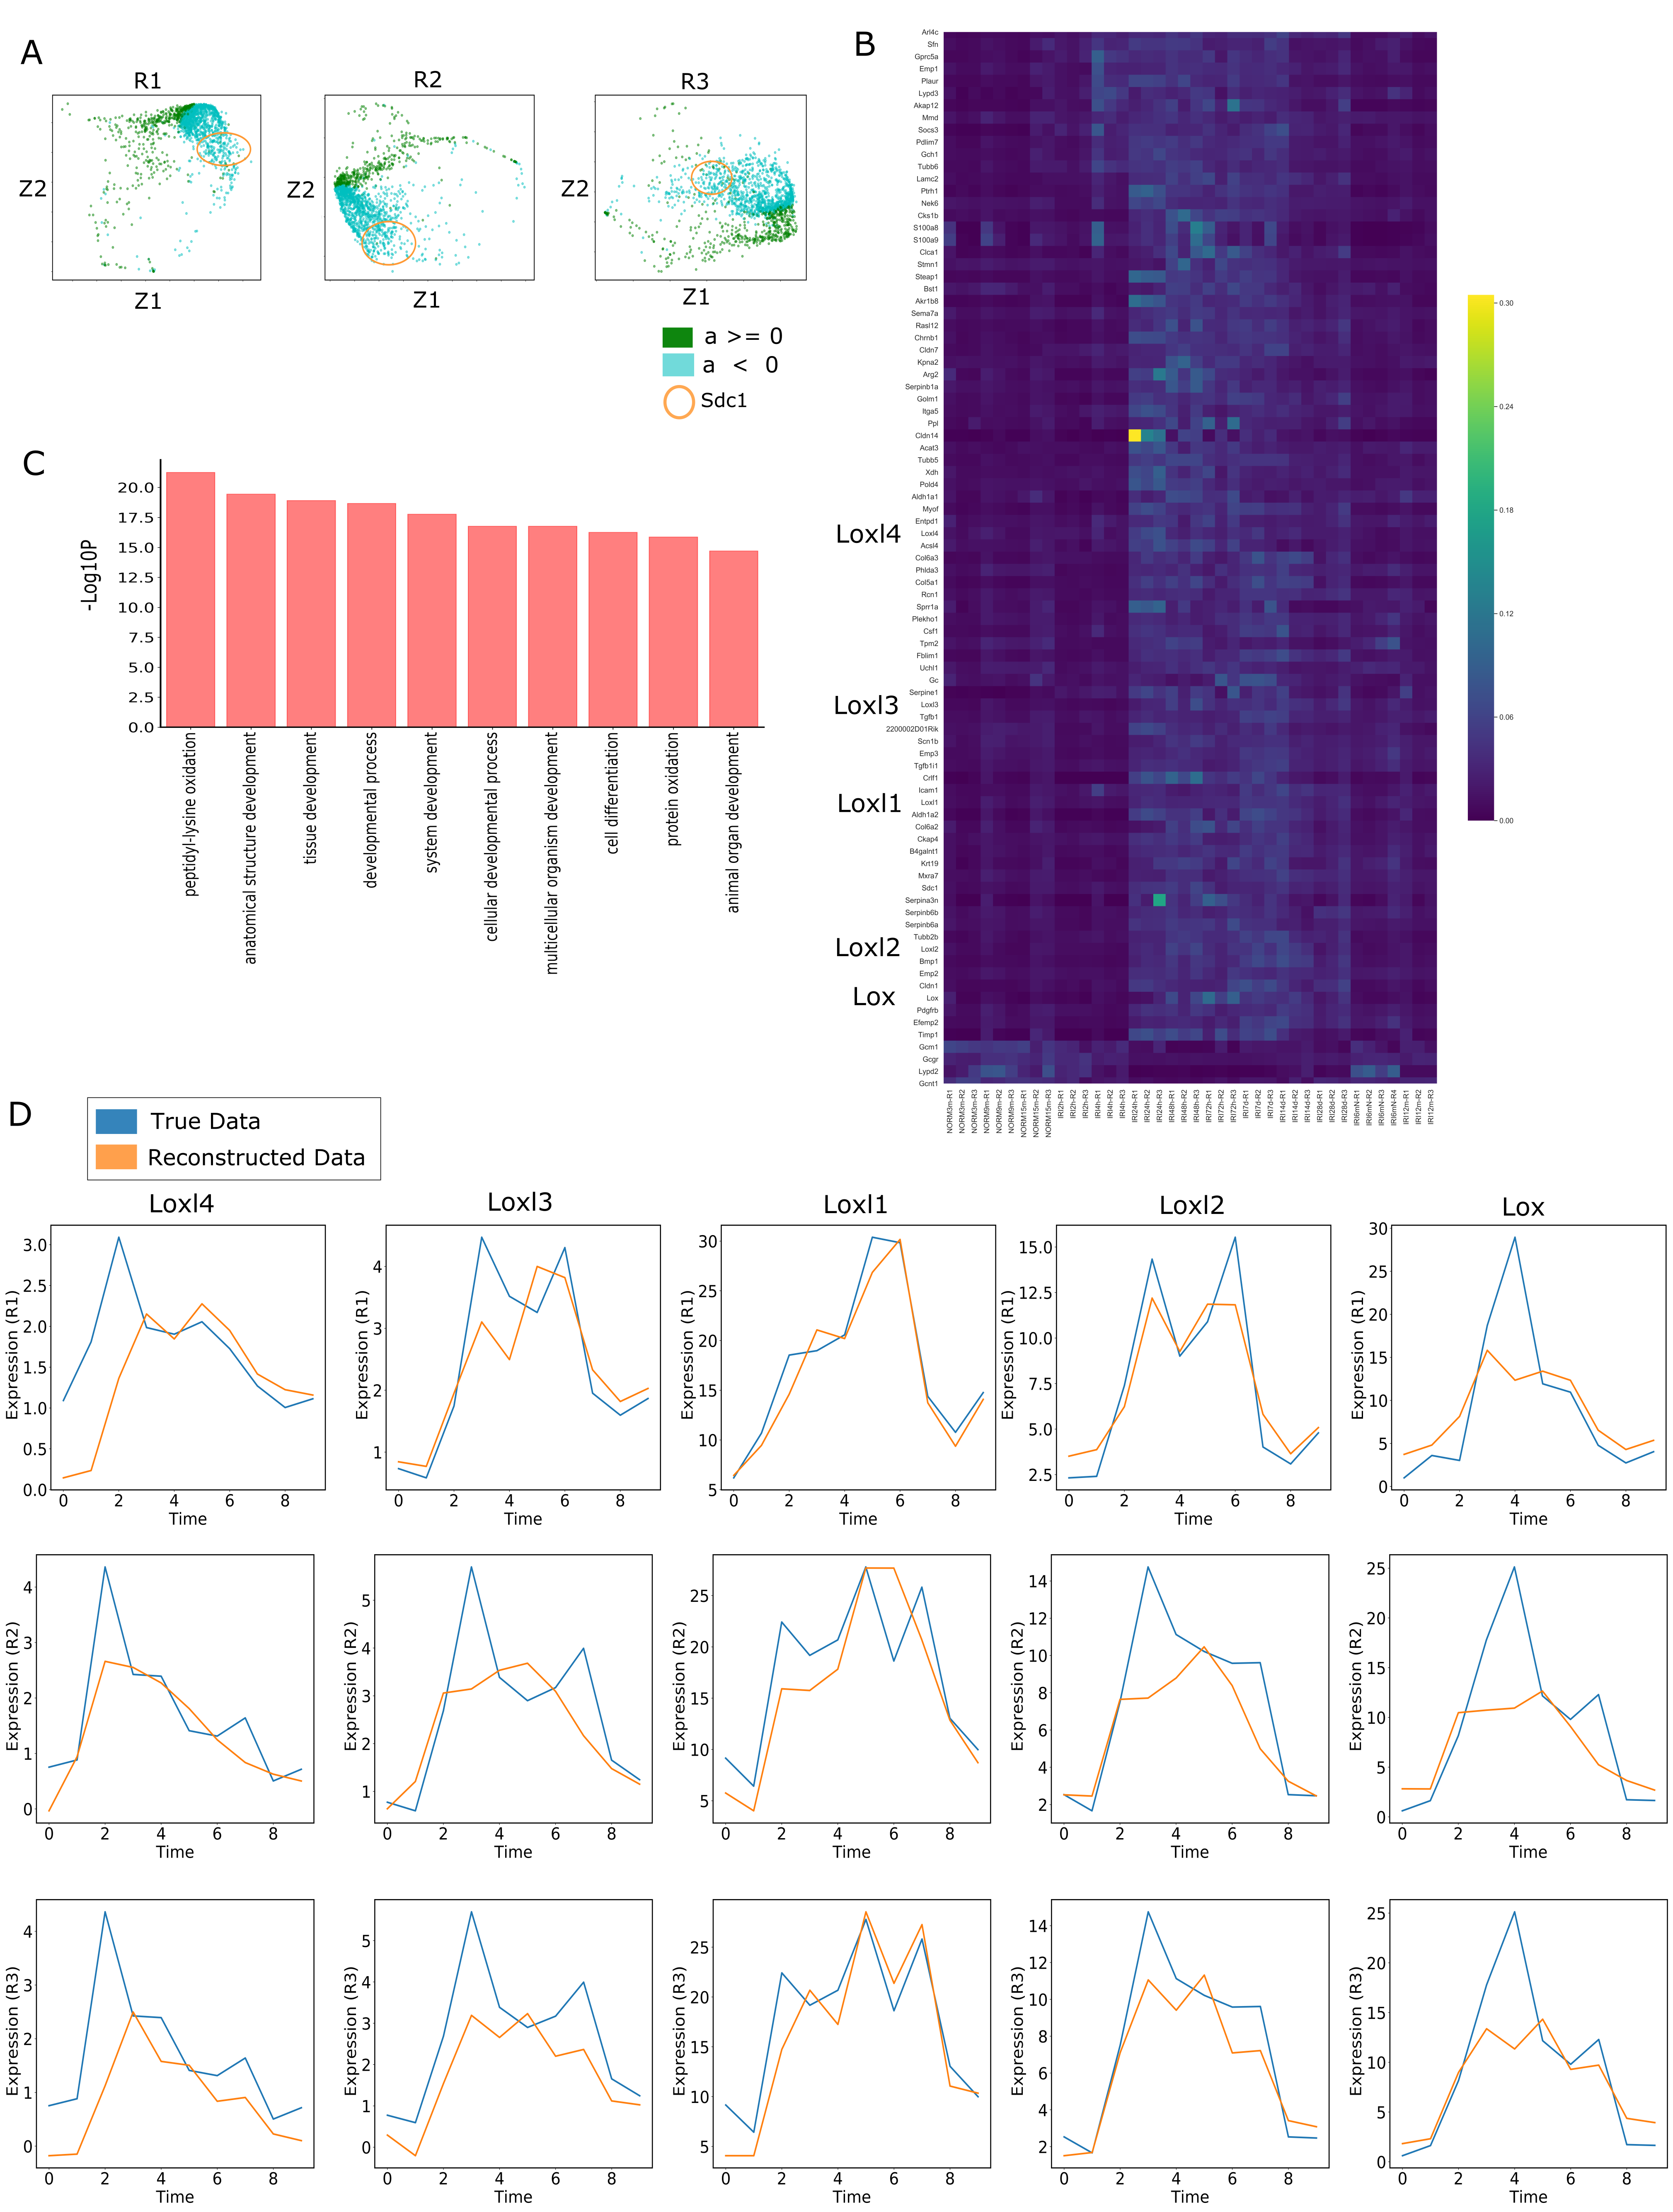
\includegraphics[width=\linewidth]{./figures/sdc_sl.png}
 % archetecture.png: 1149x508 px, 72dpi, 40.53x17.92 cm, bb=0 0 1149 508
    \caption[RVAgene latent space captures biological processes driving concordant gene expression changes (Sdc1).]{{\bf (A)} Latent space representations for replicates R1-R3 with local neighborhoods of Sdc1 marked (circles). ({\bf B}) Heatmap of expression changes over time course of injury for the Sdc1 neighborhood genes in the intersection of R1-R3; selected genes highlighted.  ({\bf C}) Histogram of -log10 p values of top GO terms for biological processes for gene set in (B).
    {\bf D}) Reconstructed vs true data plotted for each of the Lox genes identified in (B).}
  \label{fig:figS7}
\end{figure}
\end{center}

\begin{center}
\begin{figure}[H]
  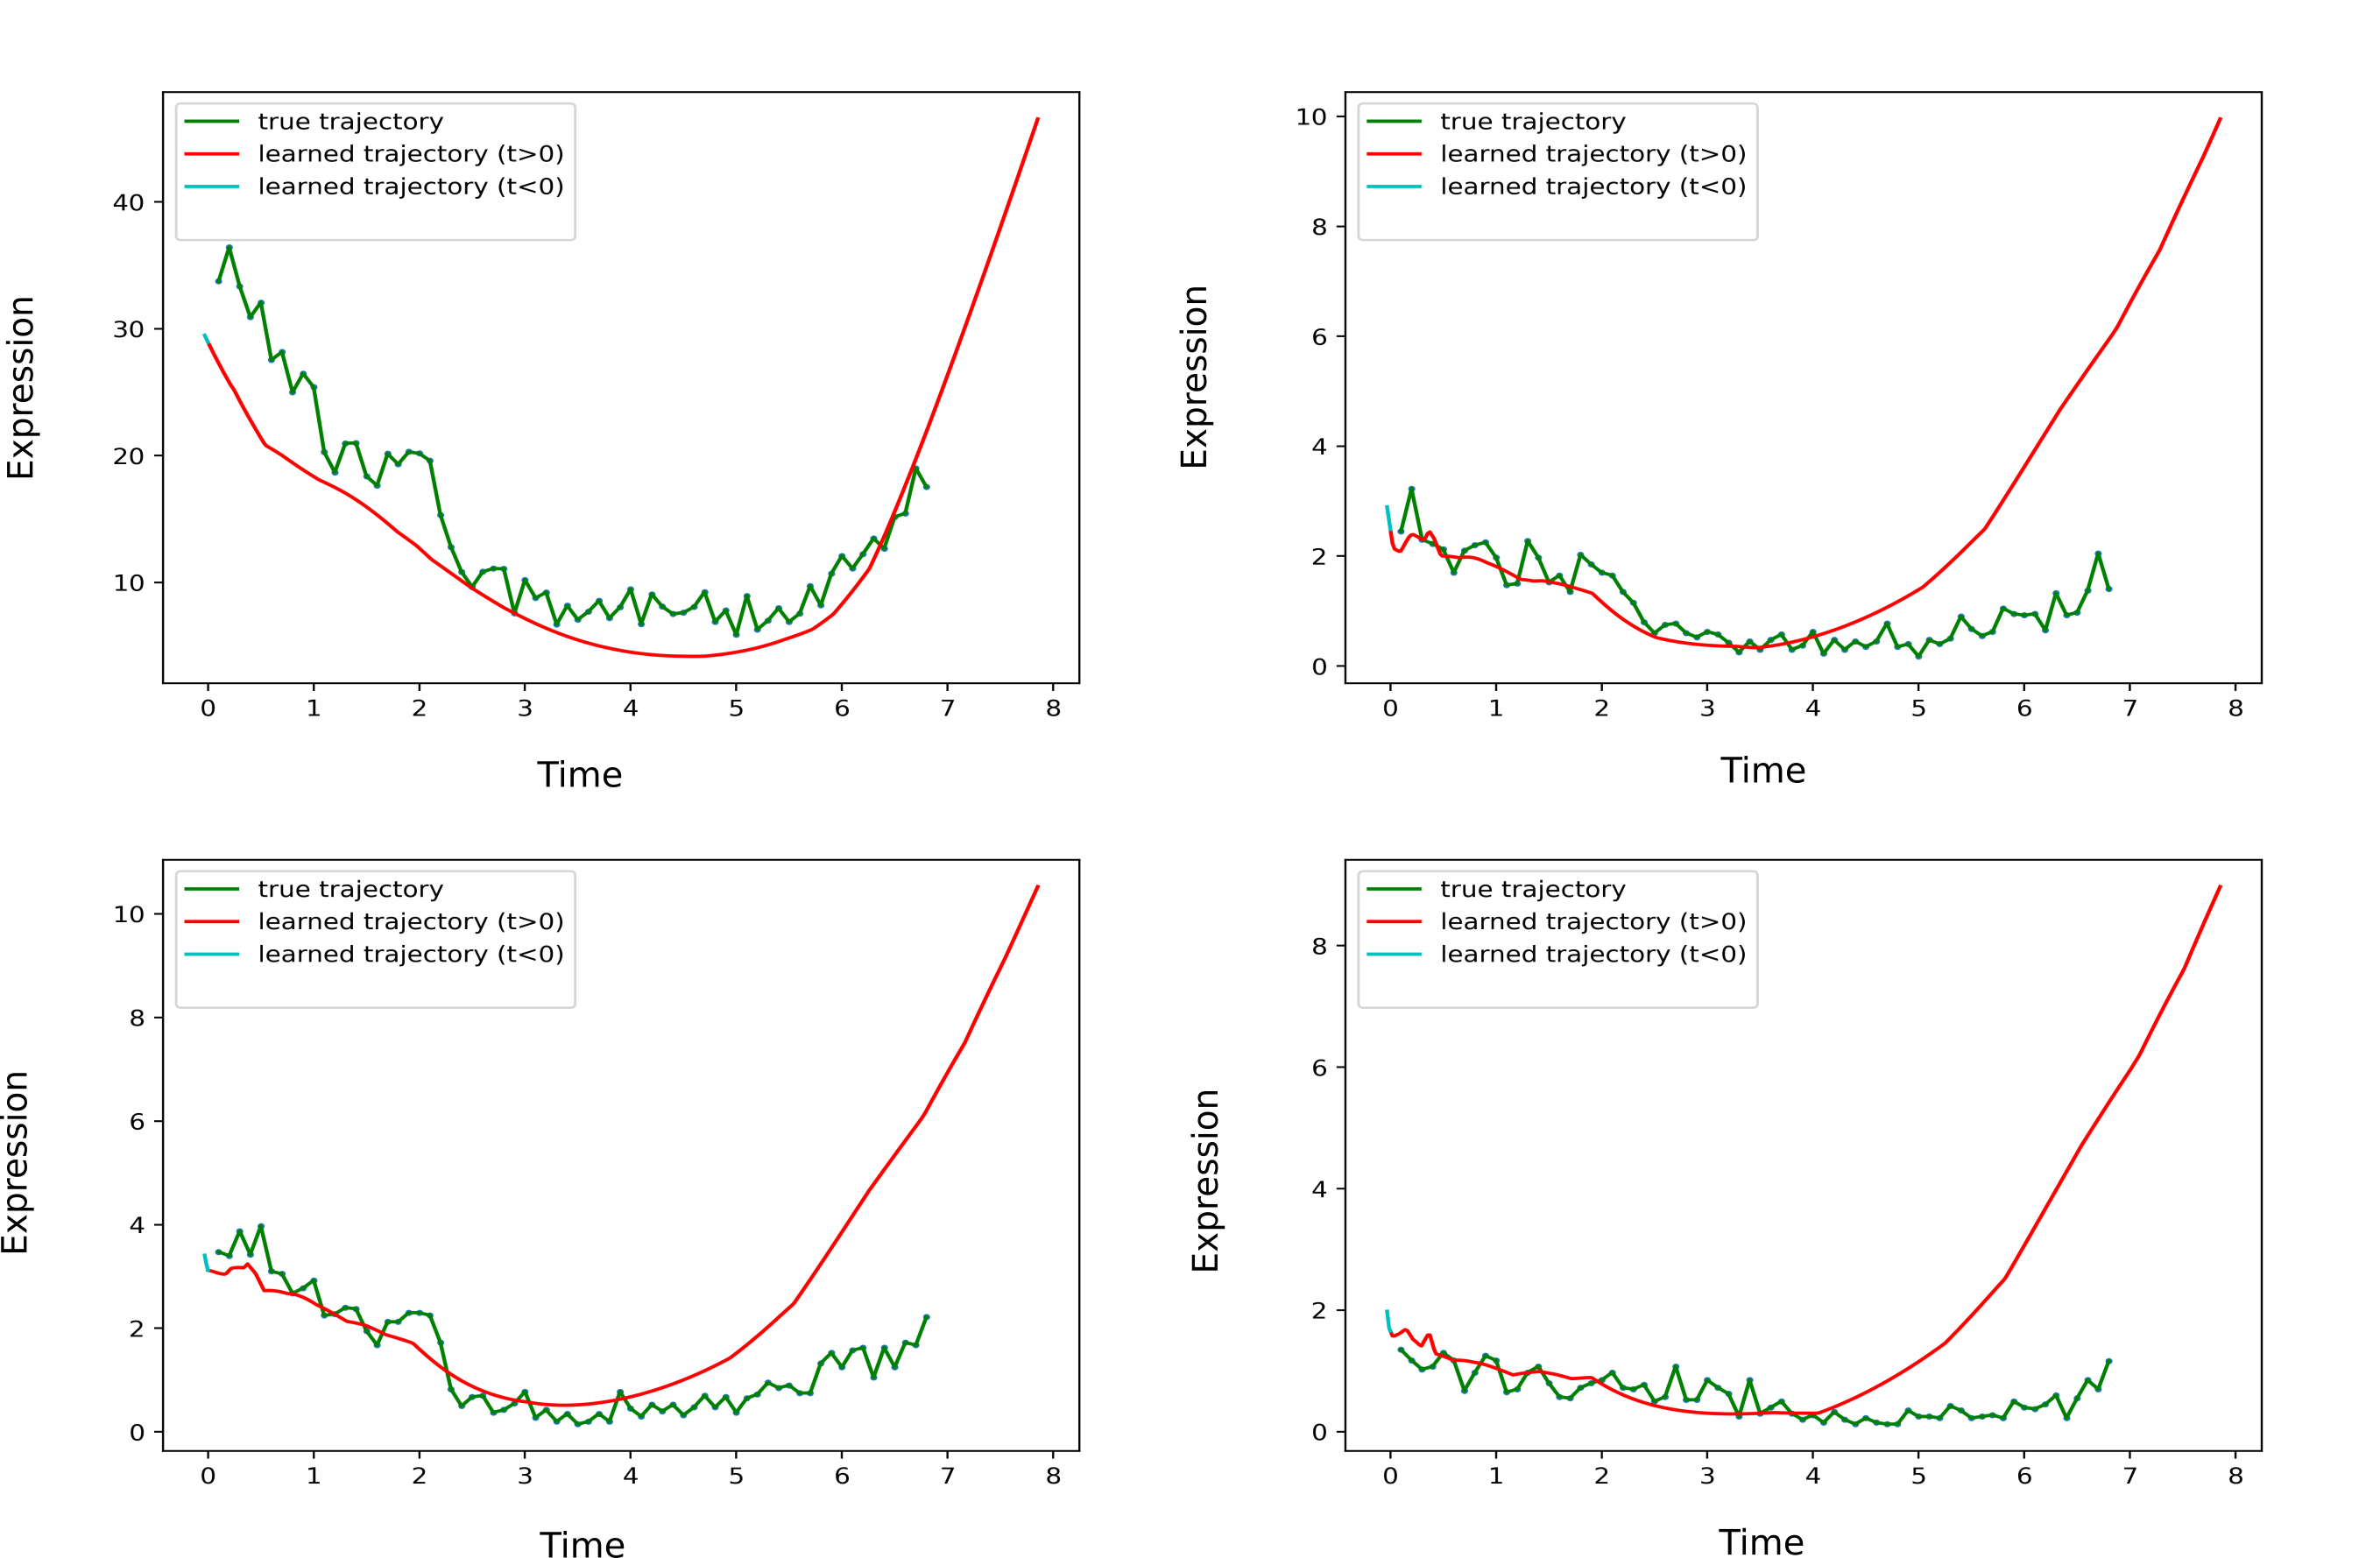
\includegraphics[width=\linewidth]{./figures/latent_ode_val_underfit.png}
  % archetecture.png: 1149x508 px, 72dpi, 40.53x17.92 cm, bb=0 0 1149 508
    \caption[Examples of continuous time prediction of ESC differentiation.]{\textbf{Examples of continuous time prediction of ESC differentiation.} Reconstruction (up to $t=6.8$) and future prediction (for $t>6.8$) for 4 example genes by a  latent ODE \citep{chen2018neural} trained on ESC data \citep{Klein2015} for 1000000 iterations, showing a good fit for the initial timepoints, but underfitting for the later timepoints.}
  \label{fig:figS9}
\end{figure}
\end{center}

\begin{center}
    \begin{figure}[H]
    \makebox[\textwidth]{\includegraphics[width=0.7\textwidth]{./crffigs/lys.png}}
 % archetecture.png: 1149x508 px, 72dpi, 40.53x17.92 cm, bb=0 0 1149 508
        \caption[Interaction propensities of components of lysine amino acid towards various DNA moieties and functional groups]{\textbf{ Interaction propensities of components of lysine amino acid towards various DNA moieties and functional groups.} ({\bf a}) Interaction  propensity towards DNA bases  A,C,G,T, in addition to phosphate (P) and sugar (S) moieties, categorized by major groovre , minor groove and all (major,minor groove and DNA backbone) ({\bf b}) Interaction  propensity towards functional groups \citep{Chiu2023} A ((H-bond acceptor), D (H-bond donor), M (methyl),H (hydrogen)), in addition to phosphate (P) and sugar (S) moieties, categorized by major groovre , minor groove and all (major,minor groove and DNA backbone)}
  \label{fig:lys}
\end{figure}
\end{center}

\begin{center}
    \begin{figure}[H]
    \makebox[\textwidth]{\includegraphics[width=0.7\textwidth]{./crffigs/his.png}}
 % archetecture.png: 1149x508 px, 72dpi, 40.53x17.92 cm, bb=0 0 1149 508
        \caption[Interaction propensities of components of histidine amino acid towards various DNA moieties and functional groups]{\textbf{ Interaction propensities of components of histidine amino acid towards various DNA moieties and functional groups.} ({\bf a}) Interaction  propensity towards DNA bases  A,C,G,T, in addition to phosphate (P) and sugar (S) moieties, categorized by major groovre , minor groove and all (major,minor groove and DNA backbone) ({\bf b}) Interaction  propensity towards functional groups \citep{Chiu2023} A ((H-bond acceptor), D (H-bond donor), M (methyl),H (hydrogen)), in addition to phosphate (P) and sugar (S) moieties, categorized by major groovre , minor groove and all (major,minor groove and DNA backbone)}
  \label{fig:his}
\end{figure}
\end{center}

\begin{center}
    \begin{figure}[H]
    \makebox[\textwidth]{\includegraphics[width=0.7\textwidth]{./crffigs/asn.png}}
 % archetecture.png: 1149x508 px, 72dpi, 40.53x17.92 cm, bb=0 0 1149 508
        \caption[Interaction propensities of components of asparagine amino acid towards various DNA moieties and functional groups]{\textbf{ Interaction propensities of components of asparagine amino acid towards various DNA moieties and functional groups.} ({\bf a}) Interaction  propensity towards DNA bases  A,C,G,T, in addition to phosphate (P) and sugar (S) moieties, categorized by major groovre , minor groove and all (major,minor groove and DNA backbone) ({\bf b}) Interaction  propensity towards functional groups \citep{Chiu2023} A ((H-bond acceptor), D (H-bond donor), M (methyl),H (hydrogen)), in addition to phosphate (P) and sugar (S) moieties, categorized by major groovre , minor groove and all (major,minor groove and DNA backbone)}
  \label{fig:asn}
\end{figure}
\end{center}

\begin{center}
    \begin{figure}[H]
    \makebox[\textwidth]{\includegraphics[width=0.7\textwidth]{./crffigs/ser.png}}
 % archetecture.png: 1149x508 px, 72dpi, 40.53x17.92 cm, bb=0 0 1149 508
        \caption[Interaction propensities of components of serine amino acid towards various DNA moieties and functional groups]{\textbf{ Interaction propensities of components of serine amino acid towards various DNA moieties and functional groups.} ({\bf a}) Interaction  propensity towards DNA bases  A,C,G,T, in addition to phosphate (P) and sugar (S) moieties, categorized by major groovre , minor groove and all (major,minor groove and DNA backbone) ({\bf b}) Interaction  propensity towards functional groups \citep{Chiu2023} A ((H-bond acceptor), D (H-bond donor), M (methyl),H (hydrogen)), in addition to phosphate (P) and sugar (S) moieties, categorized by major groovre , minor groove and all (major,minor groove and DNA backbone)}
  \label{fig:ser}
\end{figure}
\end{center}

\begin{center}
    \begin{figure}[H]
    \makebox[\textwidth]{\includegraphics[width= 0.9\paperwidth]{./rnaprodbfigs/figS1.png}}
 % archetecture.png: 1149x508 px, 72dpi, 40.53x17.92 cm, bb=0 0 1149 508
        \caption[RNAproDB search page showing card view results for the keyword search ``tetrahymena"]{\textbf{ RNAproDB search page showing card view results for the keyword search ``tetrahymena".}}
  \label{fig:rnaprodbS1}
\end{figure}
\end{center}

\begin{center}
    \begin{figure}[H]
    \makebox[\textwidth]{\includegraphics[width= 0.9\paperwidth]{./rnaprodbfigs/figS2.png}}
 % archetecture.png: 1149x508 px, 72dpi, 40.53x17.92 cm, bb=0 0 1149 508
        \caption[RNAproDB output page for uploaded AlphaFold3 predicted structure (model 0) for PDB ID: 8AW3]{\textbf{ RNAproDB output page for uploaded AlphaFold3 predicted structure (model 0) for PDB ID: 8AW3.}}
  \label{fig:rnaprodbS2}
\end{figure}
\end{center}

\begin{center}
    \begin{figure}[H]
    \makebox[\textwidth]{\includegraphics[width= 0.9\paperwidth]{./rnaprodbfigs/figs3.png}}
 % archetecture.png: 1149x508 px, 72dpi, 40.53x17.92 cm, bb=0 0 1149 508
         \caption[Multiple mapping algorithms available in RNAproDB for protein-NA-hybrid complex (PDB ID: 4OO8)]{\textbf{Multiple mapping algorithms available in RNAproDB for protein-NA-hybrid complex (PDB ID: 4OO8).} ({\bf A}) Crystal structure of of Streptococcus pyogenes Cas9 in complex with guide RNA (red) and target DNA (blue) (PDB ID: 4OO8).  ({\bf B})  Mapping produced based on partial projection. ({\bf C}) Mapping produced based on RNAscape algorithm. ({\bf D}) Mapping produced by applying ViennaRNA secondary structure layout algorithm. Centroid distance cut off of $9 \AA$ was used for protein-NA interaction edges.}
  \label{fig:rnaprodbS3}
\end{figure}
\end{center}
